%\special{ pdf: bgcolor [ 1.00 0.98 0.95 ] }
\special{ pdf: bgcolor [ 1.00 1.00 1.00 ] }

\ifx\pdfoutput\undefined % We're not running pdftex
%\documentclass[11pt,a4paper,twoside,openany]{book}
\documentclass[11pt,a4paper,oneside,openany]{book}
\else
%\documentclass[11pt,a4paper,twoside,openany]{book}
\documentclass[11pt,a4paper,oneside,openany]{book}
\usepackage{thumbpdf}
\pdfcompresslevel=9
\fi

\addtolength{\textwidth}{1.75cm}
\addtolength{\hoffset}{-0.875cm}

\usepackage{RTranslationCN}
\usepackage{shortvrb,latexsym}
\usepackage{mylayout}
\usepackage{graphicx}
\ifx\pdfoutput\undefined 
\usepackage[dvipdfm,
            colorlinks,linkcolor=blue,citecolor=magenta,
            hyperindex,
            plainpages=false,
            CJKbookmarks]
            {hyperref}
\else

%%%%%%%%%%%%%%%%%%%%%������CJKbookmarksѡ��%%%%%%%%%%%%%%%%%%%%%%%%
\RequirePackage[CJKbookmarks,colorlinks,citecolor=magenta,hyperindex,plainpages=false]{hyperref}
\def\pdfBorderAttrs{/Border [0 0 0] } % No border arround Links
\fi
\hypersetup{pdfstartview=FitH}

\usepackage{CJK,CJKnumb,indentfirst}
\makeatletter
\def\@makechapterhead#1{%
  \vspace*{50\p@}%
  {\parindent \z@ \centering%\raggedright
    \normalfont
    \ifnum \c@secnumdepth >\m@ne
      \if@mainmatter
      \huge\bfseries\prechaptername\CJKdigits{\thechapter}\chaptername\hskip 5\p@%
%        \par\nobreak
%        \vskip 20\p@
      \fi
    \fi
    \interlinepenalty\@M
    \huge \bfseries #1\par\nobreak
    \vskip 40\p@
  }}
\def\@makeschapterhead#1{%
  \vspace*{50\p@}%
  {\parindent \z@ \centering%\raggedright
    \normalfont
    \interlinepenalty\@M
    \huge \bfseries  #1\par\nobreak
    \vskip 40\p@
  }}
\makeatother
\usepackage{setspace}
\onehalfspacing
%%%%%%%%%%%%%%%%%%%%%%%%%%%%%%%%%%%%%%%%
%convert bookmarks from GBK to unicode
%%%%%%%%%%%%%%%%%%%%%%%%%%%%%%%%%%%%%%%%

\AtBeginDvi{\special{pdf:tounicode GBK-EUC-UCS2}}   % GBK -> Unicode
%%%%%%%%%%%%%%%%%%%%%%%%%%%%%%%%%%%%%
\typeout{Copyright T.Oetiker, H.Partl, E.Schlegl, I.Hyna}
%%%%%%%%%%%%%%%%%%%%%%%%%%%%%%

\renewcommand\floatpagefraction{.9}
\renewcommand\topfraction{.9}
\renewcommand\bottomfraction{.9}
\renewcommand\textfraction{.1}
 
\usepackage{multindDGH}
\makeindex{c}
\makeindex{f}
\newcommand{\cindex}[1]{\index{c}{#1}}
\newcommand{\findex}[1]{\index{f}{#1}}

\newcommand{\email}[1]{\href{mailto:#1}{#1}}

\usepackage{multicol}
\usepackage{longtable}

%%%%%%%%%%%%%%%%%%%%%%%%%%%%%%
\begin{document}
%%%%%%%%%%%%%%%%%%%%%%%%%%
\begin{CJK*}{GBK}{com}
\CJKtilde
\CJKindent

\newcommand\prechaptername  {\CJKchar{181}{218}}
\renewcommand\chaptername   {\CJKchar{"0D5}{"0C2}}
\renewcommand\contentsname  {\CJKchar{"0C4}{"0BF}\CJKchar{"0C2}{"0BC}}
\renewcommand\abstractname  {\CJKchar{"0D5}{"0AA}\CJKchar{"0D2}{"0AA}}
\renewcommand\listfigurename{\CJKchar{"0CD}{"0BC}\CJKchar{"0D0}{"0CE}%
                             \CJKchar{"0C1}{"0D0}\CJKchar{"0B1}{"0ED}}
\renewcommand\listtablename {\CJKchar{"0B1}{"0ED}\CJKchar{"0B8}{"0F1}%
                             \CJKchar{"0C1}{"0D0}\CJKchar{"0B1}{"0ED}}
\renewcommand\figurename    {\CJKchar{"0CD}{"0BC}}
\renewcommand\tablename     {\CJKchar{"0B1}{"0ED}}
%\renewcommand\bibname       {\CJKchar{"0B2}{"0CE}\CJKchar{"0BF}{"0BC}%
%                             \CJKchar{"0CE}{"0C4}\CJKchar{"0CF}{"0D7}}
\renewcommand\bibname       {��¼3 �ο�����}

\newcommand{\hlabel}[1]{\hypertarget{#1}{}\label{#1}}
\newcommand{\hlink}[2]{\hyperlink{#1}{#2}$<$ҳ�룺\pageref{#1}$>$}

%%%%%%%%%%%%%%%%%%%%%%%%%%
\frontmatter
%%%%%%%%%%%%%%%%%%%%%%%%%%%%%%%%%%%%%%%%%%%%%%%%%%%%%%%%%%%%%%%%%
% Contents: The title page
% $Id: title.tex,v 1.2 2002/05/26 22:44:33 zuohuijun Exp $
%%%%%%%%%%%%%%%%%%%%%%%%%%%%%%%%%%%%%%%%%%%%%%%%%%%%%%%%%%%%%%%%%

\ifx\pdfoutput\undefined 
\else
\pdfbookmark{����}{title}
\fi

\newlength{\centeroffset}
\setlength{\centeroffset}{-0.5\oddsidemargin}
\addtolength{\centeroffset}{0.5\evensidemargin}
\thispagestyle{empty}

\vspace{\stretch{2}}

\noindent\makebox[0pt][l]{\begin{minipage}{\textwidth}
\flushleft

{\huge \bfseries \R{} ����}
\noindent\rule[-1ex]{\textwidth}{5pt}\\[2.5ex]
\flushright
\hfill\emph{\large ����~\R{} ���Ե�ע�⣺һ�����ݷ�����ͼ����ʾ�ij�����ƻ���\\
Ӣ�İ汾 2.3.0 (2006-04-24)\\
���İ汾 0.1 (2006-06-15)}

\end{minipage}}

\vfill

\noindent\makebox[0pt][l]{%
\begin{minipage}{\textwidth}{
\flushleft
W. N. Venables, D. M. Smith\\
R ���Ŀ���С�飨the R Development Core Team��\\
\noindent\rule[-1ex]{\textwidth}{2.5pt}\\[2.5ex]
}
\end{minipage}}

\pagebreak

\vspace{\stretch{2}}

\vfill

\begin{small}
\flushleft

\emph{Ӣ���ĵ��İ�Ȩ˵��:}

Copyright \copyright 1990 W.~N.~Venables 

Copyright \copyright 1992 W.~N.~Venables \& D.~M.~Smith 

Copyright \copyright 1997 R.~Gentleman \& R.~Ihaka 

Copyright \copyright 1997, 1998 M.~Maechler 

Copyright \copyright 1999�C2006 R Development Core Team

Permission is granted to make and distribute verbatim copies of this
manual provided the copyright notice and this permission notice are
preserved on all copies.

Permission is granted to copy and distribute modified versions of this
manual under the conditions for verbatim copying, provided that the
entire resulting derived work is distributed under the terms of a
permission notice identical to this one.

Permission is granted to copy and distribute translations of this manual
into another language, under the above conditions for modified versions,
except that this permission notice may be stated in a translation
approved by the R Development Core Team.

\vspace{2ex}
\emph{�ο��������£�������Ӣ��ԭ��Ϊ׼����}

��Ȩ  \copyright 1990 W.~N.~Venables               
                                                   
��Ȩ  \copyright 1992 W.~N.~Venables \& D.~M.~Smith 
                                                   
��Ȩ  \copyright 1997 R.~Gentleman \& R.~Ihaka      
                                                   
��Ȩ  \copyright 1997, 1998 M.~Maechler            
                                                   
��Ȩ  \copyright 1999�C2006 R Development Core Team

�����ز��������ĵ���Ȩ������ǰ���£������ͷ������ĵ������������������ġ�
���ң�������Щ�������ܵ������������ı�����

�������������������汾�йذ�Ȩ������ǰ���£������ͷ������ڱ��ĵ�����
�������޸İ汾�������ģ����ң���������ͨ���޸ı��ĵ����õ��Ĺ����ɹ���
��ʹ���뱾�ĵ�����������һ�µ�����������

�����������޸İ汾��Ȩ������ǰ���£������ͷ������ĵ��������Եķ���汾
�������ģ���������������о� R ���Ŀ���С�飨R Development Core Team����
׼�ĵ��ػ��뱾������ѭ���ػ��뱾��

\vspace{2ex}
\emph{���ڱ����ķ����ĵ��İ�Ȩ������}

���ĵ�Ϊ�����ĵ���GNU FDL����
��GNU�����ĵ�����֤��\url{http://www.gnu.org/copyleft/fdl.html}���·�����
����ʾ���߰�ʾ���κα�֤�����ĵ��������ɸ��ƣ��޸ģ�ɢ�������뱣��ʹ��
����������

\end{small}


\endinput


\tableofcontents

\chapter{����}
\label{Preface}

���ĵ����� Bill Venables �� David M. Smith (Insightful ��˾)
���� ~\sm{S} �� ~\sm{SPLUS} ���������Ľ��塣
����ֻ����һЩ��С���޸��Է�ӳ ~\R{} �� ~\sm{S} �IJ��죬����������
һЩ���ϡ�

�dz���л Bill Venables �� David Smith 
�������������ַ�ʽ�����ý�����޸İ汾
�Լ�����һֱ������ ~\R{} ���ϵ�֧�֡�

�������ۺ�У������ͨ�������ʼ� 
\href{mailto:R-core@R-project.org}{R-core@R-project.org}
��ϵ���ǡ��������İ�ĸ����������ͨ�������ʼ�{\email{ghding@gmail.com}}��ϵ���ߡ�

\section{�Զ��ߵĽ���}

����� ~\R{} ���Ե����ֿ��ԴӸ�¼ A �е�\hlink{A sample session}{�����ԻỰ��session��}���֣�
������ ~\R{} �Ự��~\R{} sessions����һЩ�򵥵���ʶ����Ϊ��Ҫ���ǣ�
���ֽ������Щ ~\R{} �Ự�ж�һЩ��ʱ��������ʵʱ�ķ�����

������Щ�û��������� ~\R{} �Ļ�ͼ���ܡ�����������£�
�������������йػ�ͼ���ܵ��½�(��\hlink{Graphics}{ͼ��} һ��)��
��û�б�Ҫ��ǰ�����е��½�
�����ꡣ

\vspace{2ex}
\noindent\emph{\textbf{���������߶Ի�û�а�װ R �����û���һ������ʾ}}

���û�����ȥ\url{http://cran.r-project.org/mirrors.html}�������
һ�����Է��ʵľ����ַ��������룬���� ``Precompiled Binary Distributions''
���е������������ Windows �û������Ե��``Windows (95 and later)''��
����``base''������``rwxxxx.exe''���� rw2010.exe����Ȼ����һ��� Windows
������װ���ɡ�OK����������Ը�¼ A �е�\hlink{A sample session}{�����ԻỰ��session��}�ˡ�

\section{����ǰ��һ(ժ��05����ҳ��)}
�������ܵ�Ŭ��������������ˡ�R ���ۡ��ķ��롣����һ������ R �������ŵĽ̲ģ�
ͬʱҲ�� R �ٷ��ĵ�����������û��Ľ̲ġ�һ���û�ֻҪ�����Ȿ��R ���ۡ���
������������������ӣ��Ϳ��Խ���󲿷������ˡ�
��û�а��ĵ����� R ���ţ���Ϊ����ĵ�����Щ�����Ѿ�����һ���û���Ҫ��
���ǰ� R ��Ϊһ��ϵͳ������Щȷʵ����������ġ���һЩʱ���һ��г�һ���ʺ�
һ��ͳ���û����������嵥��

����������һ�� ROTATION ��ʱ��Ӵ� R �ģ�������һֱ�����������������Ȼ
�һ����� Stata��MATLAB��SPSS �� SAS ��ͳ�Ƽ��㷽������������� R ��Ȼ
���ҵ���ѡ����ѡ�� R �������ǣ�
\begin{itemize}
\item
R ������������������������ȡ�κη��ã�������������������κ�ͬ������ҵ�����
�ӹ������ƵĽǶ���˵��R �� MATLAB ����ġ�
\item
ͨ�� R ����Ժ�ȫ��һ����ͳ�Ƽ��㷽���ר�Һ������ۣ�����ȫ����
ͳ��ѧ��˼ά������С��Ҽ����� R ���ʼ��б���ÿ�춼���յ�����ʮ
�ݹ��� R ����Ѷ�ʼ���
\item
���dz��׵���������ͳ�Ʊ�����ԡ��������������������������ģʽ��������
���Ƿdz����������ʹ�õġ�
\item
R �������������/���ݿ�֮���кܺõĽӿڡ�
�������ϵ�ʱ��о� R Ϊ���ṩ��һϵ�ж���������������ֻҪ������Щ����Ϳ����ˡ�
����������Ϲ����dz����á�
\end{itemize}

������Ҫ˵�����ǣ���Ȼ R ��������������������Ҫ�ǵøм�����Ϊ R �����ǻ۵ķ���
�ߡ����ԣ���Ҷ� R ��֧�ֿ����������ж��ϣ�����������Ǯ��Ǯ�������ٻ������룬
��Ҳ�dz��ڶ�֪ʶ�Ͷ������ء�
������Է���\url{http://www.r-project.org/foundation/about.html}��

�����ĵ��ķ�����ֱ�Ӷ� Texinfo �ĵ����еġ����� Texinfo ������ PDF ת�����⻹û����ȫ�����
���������� HTML ��ʽ(�ַ�����UTF-8)�����ҵ��ĵ���
���������������������Խ���ģ���ķ������ǰ� Texinfo ת���� LaTeX����
PDF �汾���ĵ���ܿ�ʹ�Ҽ��档���⣬��ͬʱ�����������İ�ͷ������İ�������Է���
ʹ�÷�������ѡ�

����ʱ��ȽϽ��ţ���������п����в��ٴ�����Щ��ѧ����Ҳ�������ò�����
��ˣ�ϣ�������ֵܽ��÷��ִ���
����ҷ� email���һᾡ���޸ġ����ڻ�ֻ�� ��
�棬�ڴ�ҵ�שͷ�����󷢲���ʽ�İ汾����ʱ�򣬿϶� PDF �汾��Ҳ�㶨�ˡ���Ȼ��ҲҪ�ύ��
R ���Ŀ���С���ˡ�

�ҵ�Ŀ��������ҵ��ʱ�䷭�� R ����ݹؼ��ĵ�
��An Introduction to R�������ᣩ����R Data Import/Export������The R language definition����
��Writing R Extensions������R Installation and Administration/R FAQ����

ÿ��������
�ͻƻ��ʱ����һ��������Щ�ĵ�����һ�����������顣�һᾡ�췢����Щ�ĵ���������
��һ���ĵ��е�λ��ͳ���Եģ�Ҳ��һ�������Ҫ���ģ���������ǰ��������ĵ��ˡ�������
�ĵ��е�ƫ��߼��û����߿����û���������������˽� R�����Բ�����

``���������£�����������''���ҳ����� R������ѧ������Ӧ�õġ����������Ĺ����У�
��ѧ���˺ܶණ����

�dz���л������ҵ��ѧ�� Shigeru MASE �Լ����ߵĸ�λ���ѡ�

\emph{������}

\emph{Email��\email{ghding@gmail.com}}

\emph{2005��6��3��}

\section{����ǰ�Զ�(��PDF��)}
�Ұѡ�\R{}���ۡ��� \LaTeX{} ����д��һƪ����ȥ��һ����ҵ�����Ƚ϶࣬���ϵ������ˡ�
��ʱ���������Լ�����������顣���ǣ����ҿ�������\R{} �û�����~Emailʱ����һ�����θУ�
�����Լ�Ӧ�úú�������

�Ҷ�\R{} ��һЩ�۵㻹�Ǻ�һ��ǰд��һ������Ȼ��\R{}�����ݼ��Ƚϴ��ʱ�򣬿���̫
���ڴ棬������ʱ���е㾫���ϵ����⣬��ͨ�����ݿ�ȼ�������Щ���ⶼ���Խ����������
�����������ݷ��������һ��������

���ϴ��ᵽ``�г�һ���ʺ�һ��ͳ���û����������嵥''�����ڣ��Ҿ�ֱ���Ƽ�~Emmanuel Paradis
��~\href{http://cran.r-project.org/doc/contrib/Paradis-rdebuts_en.pdf}{R for beginners}��
���İ���XF Wang ��У����Ҳд�˼��¡�������ʽ�������Ҳ�ȷ����
��Ȼ��\href{http://cran.r-project.org/doc/contrib/Paradis-rdebuts_en.pdf}{R for beginners}
Ҳ���ҵ�\R{}���Ŷ���֮һ:\_{})��

����Texinfo���Ļ����⣬�����һ���û�н����������˽���˿��Ը�����һ���������ǣ�ֻ���� \LaTeX{}
��д����Ŭ����ԭ�ĵ��ĸ�ʽ����һ�¡�������������������Ȼ��һ������⣬����һֱû�취��``$|$''��``!''
��������һ���뵽�ĵ��оͱ�����

��PDF��󲿷ֶ��ڵ¹���ɡ�����ر��лDr. ZP Li��Dr. Rui��Li�ֵ����ҿ��Կ�����Ӧ���������������ҳ��ߣ�
���ҿ����Լ��������������ij��շdz��ã������ڹ���Ҳ�ܳԵ����ڵ������ӣ��ҽ����������в͹ݣ���
Rui ��������������һ��İ���ij���������Ժܿ���ţ����һ����Ұ�����
һЩ�dz�������Ľ���������ѧ�����ٶ�����

��Ҫ��л�ҵĵ�ʦ Prof Li���������Ҳ���֧�֡���ʱ�����е������

��лţ���ѧ�� Brian D. Ripley �� Technische Uni. Wien �� Friedrich Leisch �Ƽ���Щ�ĵ�����~\R{}
�Ĺٷ���վ��

��л��ȥһ�����������ѶԸ��ĵ�����ܶ��޸�������ر��лRonggui���ѡ�

���⣬H Li Ϊ������;���һ�����˲��ٽ��飨��Ȼ���ҿ����е����������ذ���һ�¸�������
��һ��Ҫ�Ὠ���-\_{}\^{}����Q Wang �� K Tu ��λ���Ҳ���ͳ��ѧ���潨��(˵��һ�£����ϵ�CHM�汾��
��\R{}���ۡ�����K Tu�����������У�G Li��ȥ��ͽ���
��д����ĵ���ʱ�򶼸��˲��ٰ�����Ŷ���һ���������Q Liuʦ�㣬������~Roation~��ʱ��װ\R{}��
�Ӷ��Ӵ�\R{}��

��󣬸�л \LaTeX{}�����Ļ�����С���Լ���λ��ע \R{} �����ѡ�

�����ĵ����κ�����ͽ�����Ը���Email��

\emph{������}

\emph{Email��\email{ghding@gmail.com}}

\emph{2006��7��11��}
\endinput%

%\listoffigures
%\listoftables
\enlargethispage{\baselineskip}
\mainmatter
\chapter{����}
\hlabel{Introduction and preliminaries}

\section{R ����}
\hlabel{The R environment}

~\R{} ������һ�����ݲ����������ͼ��չʾ�Ĺ��߹��ɡ�
�������ͬ��������
������ɫ���ڣ�

\begin{itemize}
\item
��Ч�����ݴ����ͱ�����ƣ�
\item
����������;�������������
\item
����������������ݷ������ߣ�
\item
ͼ�ι��߿��Զ�����ֱ�ӽ��з�����չʾ��ͬʱ������
����ͼ���豸��
\item
����һ���൱���ƣ������ָ�Ч�ij���������� (Ҳ���� `S')��
������������䣬ѭ����䣬�û�����ĵݹ麯���Լ�������������ӿڡ�
��ʵ���ϣ�ϵͳ�ṩ�Ĵ����
���������� ~\sm{S} д�ģ���
\end{itemize}

������, ���� ``����''��environment���������~\R{}��һ�־���
�����Ʋ��ҽṹͳһ��ϵͳ��������һ�����ܷdz�רһ, ��������Ĺ���Ⱥ������
�����, �����������ݷ����������泣����������

~\R{} �ǿ����µĽ���ʽ���ݷ�������һ���dz��õĹ��ߡ�
���Ŀ������ڶ̣��д�������չ\emph{��}��packages��
����ʹ�á�������������� ~\R{} �����ij���
������Ϊ�˴���һЩ�ض������ݣ���˺ܿ�
�ͱ���̭�ˡ�

\section{����������ĵ�}
\hlabel{Related software and documentation}
~\R{} ���Կ����DZ���ʵ���ң�Bell Laboratories���� Rick Becker��
John Chambers �� Allan Wilks ������ ~\sm{S} ���Ե�һ��ʵ�֡�
��Ȼ��~\sm{S} ����Ҳ�� \sm{SPLUS} �Ļ�����

���� ~\sm{S} ���Եķ�չ���̿��Բο�John Chambers ����
�������DZ�д���ı��顣���� ~\R{}������Ҫ�IJο�����
Richard A.~Becker��John M.~Chambers �� Allan R.~Wilks ���� \emph{The
New ~\sm{S} Language: A Programming Environment for Data Analysis and
Graphics}�����⣬John M.~Chambers and Trevor J.~Hastie 
��� \emph{Statistical Models in ~\sm{S}} ������
1991 ������ ~\sm{S} 3 �汾\footnote{����ע:~John M.~Chambers ����1988�����İ汾��Ϊ S3��} ��һЩ��������
\pkg{methods} ���еķ�����method�����ࣨclass�� ���ǻ��� John M.~Chambers ����
\emph{Programming with Data}��
����ο���Ŀ����¼�е�\hlink{References}{�ο�����}����.

�����Ѿ��кܶ��������� ~\R{} �������ݷ�����ͳ�Ƶ��鼮��
~\sm{S}/\sm{SPLUS}������ĵ�������ֱ������~\R{}������
Ҫע�� ~\R{} �� ~\sm{S} ʵ���ϵIJ��졣
�μ�~\R{} �ij������⼯��
\href{R-faq_cn.pdf}{R �������⼯}��

\section{R ��ͳ��}
\hlabel{R and statistics}
\cindex{��}

���Ƕ� ~\R{} �����Ľ�����û���ᵽ
\emph{ͳ��}�����Ǵ�������� ~\R{} ������Ϊ����ͳ�ƹ��ܡ�
�������������ɰ� ~\R{} ����һ���ڲ�ʵ�������ྭ���ʱ�ֵ�
ͳ�Ƽ����Ļ��������ֵ�ͳ�ƹ�����������
~\R{} �����ĵײ㣬���Ǵ������������ \emph{��} ����ʽ�ṩ��
��Լ��25������ ~\R{} ͬʱ����������Ϊ``��׼'' �� ``�Ƽ�''
����������İ�����ͨ�����ϻ������ط���
\emph{CRAN} ���� (\url{http://CRAN.R-project.org})
�õ������ڰ������ϸ��
���ں�����½����� (��\hlink{Packages}{��}һ��)��

����������ͳ�Ʒ��������µļ���������
�� ~\R{} ��ֱ�ӵõ����ն��û�ֻ����Ҫ
���㾫��ȥ�ҵ�һ�¾Ϳ����ˡ�

~\sm{S}(Ҳ���� ~\R{}) ��������Ҫ��ͳ��ϵͳ�ڹ�����
������Ҫ�IJ��졣�� ~\sm{S}�����У�һ��ͳ�Ʒ���
�������ֽ��һϵ�в��裬�������е��м�������������
����object���С���ˣ�SAS �� SPSS Ϊ�ع��
�б�����ṩ�˷ḻ����Ļ������ݣ��� ~\R{} ����
��Ļ���ȴ���١��������������һЩ���ʵĶ�����
�Ա����� ~\R{} ����ĺ�������һ���ķ���\footnote{����ע: �����~\R{}�������dz�����Ҫ.}��

\section{R ������ϵͳ}

�����׵ķ���������һ������ϵͳ��ͼ�ι���վ��graphics workstation����
���� ~\R{}����Ȼ����Ҫ�Ƕ������ֱ����Ķ���˵�ġ�
�������������Dz�����ָ��
ʲô ~\R{} ������ʹ�� ~\R{}��
������ż�����ᵽ�� X window ϵͳ��ʹ�� ~\R{}��

������û���������б�Ҫ�ͼ����ϵͳ����ֱ�ӽ���.
�ڱ��ֲ���,
������Ҫ������ UNIX ����ϵͳ�еĽ���ʽ������
������� Windows ���� MacOS ������ ~\R{} �������
��Ҫ�������ĵ�����

Ϊ������� ~\R{} �ĸ��Ի����ã�ֱ������ͼ�ι���վ��
��ֱ�ӵİ취�����������ַ����е㷦ζ�����Dz�׼������������⡣
�û���������ⷽ�������
�����������߸���Ѱ�������

\section{����ʽʹ�� ~\R{}}
\hlabel{Using R interactively}

��һ�� ~\R{} ������Ҫ����������ʱ��������ʾ������ʾ���� 
Ĭ�ϵ���ʾ���� \code{>}��UNIX ϵͳ�п��ܻ�
�� shell ��������ʾ��һ�¡�����������ǰ����û���������С�
���ǣ�����������������һ������������趨����Ҫ��
��ͬ��Ĭ��ֵ�� ~\R{} ������ʾ�����ڽ��������ĵ��У����ǽ��ٶ� UNIX
�� shell �������ʾ���� \code{\$}��

������ǵ�һ���� UNIX ϵͳʹ�� ~\R{}�������Ƽ��IJ�������
���£�

\begin{enumerate}
\item
����һ����������Ŀ¼ \file{work} ��������Ҫ�����ϵͳ��
�� ~\R{} �����������ļ��������� ~\R{} ������Щ����ʱ��
�⽫����Ĺ���Ŀ¼��

\begin{example}
$ mkdir work
$ cd work
\end{example}

\item
���������� ~\R{} ����

\begin{example}
$ R
\end{example}

\item
��ʱ�����Լ��� ~\R{} ������ (�����������)��

\item
�˳� ~\R{} �����������

\begin{example}
> q()
\end{example}

���ʱ��~\R{} �Ự�������Ƿ���Ҫ�������ݡ�
��Щϵͳ�ᵯ��һ���Ự�򣬻���һЩϵͳ��
������ı�������ʾ�������ı�������ʾ������Լ���
\kbd{yes}��\kbd{no}, \kbd{cancel} �������ǵ�����ĸ
�Ա�ʾ���˳�ǰ�������ݣ����������ݾ��˳��������·���
~\R{} �Ự������������ݿ��Խ����� ~\R{}
�Ự���µ��á�

\end{enumerate}

���� ~\R{} �Ự�DZȽ����׵ġ�

\begin{enumerate}

\item
��������Ŀ¼ \file{work}����ǰ��һ���IJ�����������

\begin{example}
$ cd work
$ R
\end{example}

\item
ʹ�� ~\R{} ������ \code{q()} �������
�Ự��

\end{enumerate}

�� Windows ϵͳʹ�� ~\R{} �IJ��������ڱ�������һ���ġ�����һ������Ŀ¼��
����Ŀ¼����Ϊ ~\R{} �����ݷ�ʽ��\file{��ʼλ��}\footnote{����ע���Ҽ���� ~\R{} �����ݷ�ʽ������һ���˵���ѡ��``����''�������Ự�򣬵��
\file{``��ݷ�ʽ''}���Ϳ��Կ���\file{``��ʼλ��''}���������������Ĺ���Ŀ¼����OK\^{}\_\^{}��}
��˫�����ͼ�������� ~\R{}��

\section{һ�������Ե�~\R{} �Ự}

����������ڼ��������Լ��ĵ���������һ�� ~\R{} ��������
�Ǿ�Ѹ�ٰѸ�¼ \hlink{A sample session}{һ���򵥻Ự} �и�����
������ ~\R{} �Ự���ꡣ���ʾ���Ե� ~\R{} �Ự�dz�ֵ���Ƽ���

\section{ͨ������������Ѱ�����}
\findex{help}

~\R{} ��һ����UNIX�İ������� \code{man} ���Ƶ���Ƕ�������ߡ�
Ϊ�˵õ��κ��ض����ֵĺ����İ�������
\code{solve}������ʹ����������

\begin{example}
> help(solve)
\end{example}
\findex{help}

����һ�ְ취��

\begin{example}
> ?solve
\end{example}
\findex{?}

���������⺬����ַ������Լ���
˫���Ż��ߵ����ţ���``�ַ���''��
��ͬ�����������﷨����Ĺؼ���
\code{if}��\code{for} �� \code{function}��

\begin{example}
> help("[[")
\end{example}

�κ�һ�����Ŷ����������ݣ�escape������һ�֣���
�ַ��� \code{"It's important"}\footnote{����ע��������� \code{'It's important'}��~\R{} �ͻ�������﷨����}��
ϰ���ϣ�һ������ʹ��˫���š�

�ڴ���� ~\R{} ƽ̨�У������ͨ���������������õ�
\HTML{} ��ʽ�İ����� 

\begin{example}
> help.start()
\end{example}
\findex{help.start}

\noindent
��������һ����ҳ�������������ͨ����������
����ҳ���� UNIXϵͳ�У������İ���Ҫ����Է��͸�
���� \HTML{} �İ���ϵͳ���� \code{help.start()} ���������ҳ�ϣ�
`��������͹ؼ���'��Search Engine \& Keywords �������ر����ã���Ϊ
��ͨ����������ʹ�õĺ������ṩһ���߲�εĸ����б���
�������ܿ������Լ�������λ�ú�����
~\R{} ���ṩ�ĺ���������Χ��

\findex{help.search}
\code{help.search} ����\footnote{����ע���ҷdz�ϲ����������\code{?}�������������õ�����һ��}
���������κη�ʽ���������ĵ���
���� \code{?help.search} ��һ������������ϸ��Ϣ�����ӡ�

����ij��������������ӣ����������������鿴��

\examp{
> example(\var{topic}) \# topic ����Ҫ����Ե������barplot
}
\findex{example}

Windows �汾�� ~\R{} ����������ѡ�İ������ߣ�
�������������������
���������Ϣ\footnote{����ע: BioConductor��Ŀ���ṩ��Ϊ~Vignettes �İ�������.}��

\begin{example}
> ?help
\end{example}

\section{R �����Сд���е�}

��������˵��~\R{} ��һ���﷨�dz��򵥵�\emph{����ʽ����}��expression language����
��\emph{��Сд����}�����
\code{A} �� \code{a} �Dz�ͬ�ķ�����ָ��
��ͬ�ı����������� ~\R{} ������ʹ�õ������ַ���
������ ~\R{} �����е�ϵͳ�͹���
(����ϵͳ�� \emph{locale} ����)��ͨ�������֣���ĸ
��\samp{\code{.}} �� \samp{\code{\_}}����������(��һЩ���һ���������
��ĸ)��������һ������������
\samp{\code{.}} ������ĸ��ͷ������
�� \samp{\code{.}} ��ͷʱ�ڶ����ַ������������֡�

��������Ҫô��\emph{����ʽ}��expressions��Ҫô����
\emph{��ֵ}��assignments�������һ�������DZ���ʽ����ô������
��������evaluate�������������ʾ����Ļ�ϣ�ͬʱ��ո�������ռ�ڴ档
��ֵͬ�����������ʽ���Ұ�ֵ�������������
�����Զ���ʾ����Ļ�ϡ�

������Ա� (\samp{\code{;}})����������
����һ�С������������ͨ��������(\samp{\code{\{}}��\samp{\code{\}}})
����һ�𹹳�һ�����ϱ���ʽ��compound expression����
\emph{ע��}�������Է����κεط�\footnote{\strong{��Ҫ}�����ַ���֮�У�
Ҳ��Ҫ����һ����������IJ����б���}��
һ���У��Ӿ���(\samp{\code{\#}})��ʼ��������β֮������
����ע�͡�

���һ��������һ�н�����ʱ�����﷨�ϻ���������~\R{} ��
����һ����ͬ����ʾ����Ĭ����

\begin{example}
+
\end{example}

\noindent
����ʾ��������ڵڶ��к��������У��������ȴ�����ֱ��
һ���������﷨���������ġ�����ʾ�����Ա��û��޸ġ�
�ں�����ĵ��У����dz���ʡ��������ʾ����continuation prompt��
���Լ򵥵�������ʾ����������

\section{���µ��ú�������ǰ������}

�ڴ���� UNIX �汾�� Windows ϵͳ�ϣ�~\R{} �ṩ��һ��
���ú�����ִ����ǰ�ù�������Ļ��ơ����̵����¼�
����ʹ�����\emph{�������ʷ��¼}��command history����ǰ������
���ˡ�һ���ҵ�ij����������������ͨ��
���Ҽ��ƶ�������
���Բ��������ַ�������\key{DEL}��ɾ���ַ���
����������ݿ��Բο���¼ \hlink{The command-line editor}{�����б༭��}.

UNIX �������ǰ�ù�����ĵ��úͱ༭�ļ������ǿ����޸ĵģ�
�������ݿ��Բο�\strong{readline} ���ָ�ϡ�

�ر���һ�£�Emacs �ı��༭��\footnote{����ע����ȻVi��UltraEditҲ�������Ҿ���UltraEditд ~\R{} ���������ؿ���ģ��ġ�
��\url{http://www.ultraedit.com/index.php?name=Content&pa=showpage&pid=40}���� ~\R{} �� wordfile
��``R Scripting - 02/18/2003''��������ܻ���Щ��ͬ����������� UltraEdit �����Ŀ¼�µ� wordfile.txt �ļ��о����ˡ���ʱ���Զ���� .R �ļ��﷨������ʾ��}
�Խ���ʹ�� ~\R{} �ṩ�˸�һ��Ļ��� (��Ҫ�� \emph{ESS} �� \emph{Emacs Speaks Statistics})��������Բμ�R�����⼯: \href{R-faq_cn.pdf}{R �������⼯}��

\section{�������ļ��ͽ���ض���}
\cindex{������������}

���һ��������ڹ���Ŀ¼ \file{work} ��һ���� \file{commands.R} ���ļ��У�
�����������������
~\R{} �Ự��ִ������ļ���

\begin{example}
> source("commands.R")
\end{example}
\findex{source}

�� Windows �汾�� ~\R{} ����̨�У� ������\strong{�ļ�}��File���˵���
ѡ��\strong{����}��Source����ʵ�֡����ں��� \code{sink}�����������

\begin{example}
> sink("record.lis")
\end{example}
\findex{sink}

\noindent
���԰����к������������ӿ���̨�ض����ⲿ�ļ�\footnote{����ע����ʱ������̨���Կ���
�������������ǿ���������������Ϊ����������ⲿ�ļ���ȥ�ˡ�} \file{record.lis} �С�����

\begin{example}
> sink()
\end{example}

\noindent
������������¶��򵽿���̨��

\section{�������ݺͶ���ɾ��}

~\R{} �����Ϳ��Ƶ�ʵ�壨entity������Ϊ
\emph{����}�����ǿ����DZ��������飬�ַ�����
��������������ͨ����Щʵ�嶨���
��Ϊһ���ԵĽṹ��structures����

�� ~\R{} �Ự�����У�������ͨ�����ִ����ͱ����(���ǽ��ں����
�����������������)��~\R{} ������(����\code{ls()})

\begin{example}
> objects()
\end{example}

\noindent
��������ʾ��ǰ 
������ ~\R{} �����еĶ������֣����ܲ���ȫ�����֣���
���浱ǰ����ĵط�����Ϊ\emph{�����ռ�}��workspace����
\cindex{�����ռ�}

����ͨ������ \code{rm} ɾ������

\begin{example}
> rm(x, y, z, ink, junk, temp, foo, bar)
\end{example}
\findex{rm}
\cindex{ɾ������}

~\R{} �Ự�д��������ж���������õر�����һ���ļ���
�Ա����Ժ�� ~\R{} �Ự���á���ÿһ�� ~\R{} �Ự������ʱ��
����Ա��浱ǰ���п��õĶ���
�����������������Щ���󽫻�
д�뵱ǰĿ¼��һ���� \file{.RData}\footnote{�ļ�����ʼ��``��'' 
���ܻ����ļ��ڳ���� UNIX �ļ��б���\emph{���ɼ�}���������ļ���}
���ļ��У�������������λỰ���ù���������
���ᱻ������һ���� \file{.Rhistory} ���ļ��С�

�� ~\R{} �ٴ���ͬһĿ¼����������Щ���󽫴�����ļ���
���µ��빤���ռ䡣ͬʱ����ص���ʷ�����ļ�Ҳ��
�����롣

������� ~\R{} �����������������Զ����Ĺ���Ŀ¼��
�ڷ��������У�����������Ϊ
\code{x} �� \code{y} ��һ���dz����������顣��һ�ζ����ķ����У�
���������������ض�����ģ�������������ͬʱ��һ��Ŀ¼
�½���ʱ���������ǵĺ���
������һ���dz����ѵ����顣  

\endinput%
\chapter{�򵥵�������������������}
\hlabel{Simple manipulations numbers and vectors}
\cindex{����}

\section{�����͸�ֵ}
\hlabel{Vectors and assignment}

~\R{} ���Ѿ�������\emph{���ݽṹ}��data structure���������õġ����У�
��򵥵Ľṹ������һ��������ֵ���ɵ���ֵ\emph{����}��vector������������Ҫ
����һ�����������ֵ������ \code{x}���������ֵ�ֱ�Ϊ10.4��5.6��3.1��
6.4 �� 21.7����~\R{} �е�����Ϊ

\begin{example}
> x <- c(10.4, 5.6, 3.1, 6.4, 21.7)
\end{example}
\findex{c}
\findex{vector}

����һ����\emph{����} \code{c()} ��ɵ�\emph{��ֵ}��䡣
�����\emph{����} \code{c()} ������������
\emph{����}���������ص�ֵ����һ������Щ������β����
�γɵ�����\footnote{���� \code{c()} �Ķ�������ʽ��\code{list} ģʽ�IJ����������
���ܻ��е���졣����μ� \hlink{Concatenating lists}{�б�������}}��

�� ~\R{} �������棬��������ֵҲ�DZ���������Ϊ1��������

ע��һ�¸�ֵ���� (\samp{\code{<-}})����ʵ���ϰ���
�����ַ����� \samp{\code{<}} (``С�ں�'') ��
\samp{\code{-}} (``����'')���������ַ��ڷ�����Ҫ���ϸ�һ��
\footnote{����ע��`-$>$'��`$<$-'��һ�µģ���'`-$<$'��`$>$-'�Ͳ�һ���ˡ�}
����`ָ��'������ʽ��ֵ�Ķ���
����������£�\samp{\code{=}} ���Դ���ʹ�á�
\cindex{��ֵ}

��ֵҲ�����ú��� \code{assign()} ʵ�֡�
����������ǰ��ĸ�ֵ����ȼۣ�

\begin{example}
> assign("x", c(10.4, 5.6, 3.1, 6.4, 21.7))
\end{example}

\noindent
���dz��õĸ�ֵ�� \code{<-} ���Կ����Ǹ�����
һ�������ϵ���д��

��Ȼ�������Դ�����һ�������ϸ�ֵ��
���������䣬�����������ͬ���ĸ�ֵ����

\begin{example}
> c(10.4, 5.6, 3.1, 6.4, 21.7) -> x
\end{example}

���һ������ʽ��һ�������������ô����ֵ���ᱻ��ʾ����Ļ��
\emph{���Ҳ��ܱ���Ķ������}\footnote{ʵ���ϣ���������������ǰ��
���DZ����ڱ��� \code{.Last.value} �С�����ע����Ȼ���㻹����ֱ������Ļ��ֱ�ӿ�������ʽ�����ֵ��}��
��ˣ���������������

\begin{example}
> 1/x
\end{example}

\noindent
������ĵ����ͻ����ն���ʾ (ע�⣬\code{x} ��ֵû�иı�)��

��һ���ĸ�ֵ

\begin{example}
> y <- c(x, 0, x)
\end{example}

\noindent
�ᴴ��һ������11��Ԫ�ص����� \code{y}��
���а������� \code{x} ������λ���м��һ��0��

\section{��������}

����������ʽ��ʹ����������Ը�������ÿһ��
Ԫ�ض�����ͬ���������㡣������ͬһ������ʽ�е�
��������dz���һ�¡�������ǵij��Ȳ�һ����
�ñ���ʽ��ֵ����һ��������������ȳ���
����������ʽ�ж̵�����
�ᱻ\emph{ѭ��ʹ��}��recycled��(������
���ֵ�Ԫ��)�Դﵽ������ij��ȡ�
����һ���������Ǽ򵥵��ظ�������ǰ�������еı�����
����
\cindex{ѭ��ʹ��ԭ��}

\begin{example}
> v <- 2*x + y + 1
\end{example}

\noindent
������һ���µij���Ϊ11������ \code{v}������
\code{2*x} �ظ�2.2�Σ�\code{y} �ظ�һ�Σ�
\code{1} �ظ�11�εõ���������Ӷ��ɡ�

\cindex{���������������}
������������������dz��õ�\code{+}�� \code{-}��
\code{*}�� \code{/} �����������õ�\code{\^{}}��
\findex{+}
\findex{-}
\findex{*}
\findex{/}
\index{f}{\verb.^.}
���⻹�������õ���ѧ��������
\code{log}��\code{exp}��\code{sin}��\code{cos}��\code{tan}��\code{sqrt}
�ȵȡ���Щ�ڽ̿����϶��������塣
\findex{log}
\findex{exp}
\findex{sin}
\findex{cos}
\findex{tan}
\findex{sqrt}
\code{max} �� \code{min} �ֱ����һ��������
���ֵ����Сֵ��
\findex{max}
\findex{min}
���� \code{range} �õ�����һ������Ϊ2����������
\code{c(min(x), max(x))}��
\findex{range}
\code{length(x)} �������� \code{x} ��Ԫ�ظ�����
\findex{length}
\code{sum(x)} ���� \code{x} ��Ԫ�ص��ۼӺͣ�
\findex{sum}
�� \code{prod(x)} ��õ����ǵij˻���
\findex{prod}

����ͳ�ƺ������Ǽ����ֵ�� \code{mean(x)}
���ȼ��� \code{sum(x)/length(x)}��
\findex{mean}
�ͼ������������ \code{var(x)}��\code{var(x)} �ȼ���

\begin{example}
> sum((x-mean(x))^2)/(length(x)-1)
\end{example}
\findex{var}

\noindent
��� \code{var()} �IJ�����һ��
\rmath{n}��\rmath{p} �ľ����򽫸þ���������֮�俴�����໥������
\rmath{p}-�����������������Ӷ��õ�һ�� \rmath{p}��\rmath{p} ��
�����������

\code{sort(x)} ����һ���� \code{x} ����һ����
Ԫ�����������е����������⣬�����������ܸ�ǿ���
������(������������е� \code{order()} ��
\code{sort.list()}��)��
\findex{sort}
\findex{order}

ע�� \code{max} �� \code{min} ����������Dz�������
�е�������Сֵ����ͬʱ��������������������£�������������Ѳ��������ϲ���һ������������
\emph{����}��parallel�����������Сֵ�ĺ��� \code{pmax} ��
\code{pmin} ���᷵��һ������IJ�������һ�µ�������
������ÿһ��Ԫ�ؾ���ͬһλ���ϵ�
���������������������IJ�����Ԫ�ص������С��ֵ��
\findex{pmax}
\findex{pmin}

���������£��û���������һ����ֵ�����е�``��ֵ''
������������ʵ�������Ǹ�����~\R{} �����ڲ��ļ���
����˫���ȵ�ʵ������
˫���ȵĸ����������������Ǹ���������£�ʵ�ֵġ�

���Ҫ����������Ӧ�ø�����ȷ�ĸ������֡����

\begin{example}
> sqrt(-17)
\end{example}

\noindent
������� \code{NaN} ��һ�����棬����

\begin{example}
> sqrt(-17+0i)
\end{example}

\noindent
�ͻ��Ը�����ʽ���㡣

\section{������������}
\hlabel{Generating regular sequences}
\cindex{��������}

~\R{} ��һϵ�в����������еĹ��ߡ�
�� \code{1:30} �ȼ������� \code{c(1, 2,
\dots{}, 29, 30)}��
\findex{:}
��~\R{}����ʽ�У�ð�����ȼ�����ߣ����
\code{2*1:15} �ȼ��� \code{c(2, 4, \dots{}, 28, 30)}��
���߿������潫 \code{n <- 10}��\code{1:n-1}��
\code{1:(n-1)}�໥�Ƚ�һ�¡�

\code{30:1} ��ʽ�ľ䷨��construction������������һ��
���������

\findex{seq}
���� \code{seq()} ��������������Ϊ���õĹ��ߡ�
������������������ֲ�����Ҫÿ�ζ��趨��
��ʼ��������������ʾ
һ�����е���β�����ֻ��
����������ֵ�����ð���������Ч����ȫһ���ˡ�
�� \code{seq(2,10)} �ȼ��� \code{2:10}��

\code{seq()} ���������� ~\R{} �����IJ���һ��
�������ò���������ʽ��������������£�������˳�����������ġ�
������ǰ���������Ϳ�����
\code{from=\var{value}} �� \code{to=\var{value}} ��ʽ�趨�����
\code{seq(1,30)}��\code{seq(from=1, to=30)}��\code{seq(to=30,
from=1)} ͬ \code{1:30} ��ȫһ����\code{seq()} ������������
�� \code{by=\var{value}} ��
\code{length=\var{value}}�����Ƿֱ��ʾ������еIJ����ͳ��ȡ�
�������û���趨��Ĭ��ֵ����
\code{by=1}������Ϊ1����

����

\begin{example}
> seq(-5, 5, by=.2) -> s3
\end{example}

\noindent
������ \code{c(-5.0, -4.8, -4.6, \dots{},
4.6, 4.8, 5.0)} ���� \code{s3}�����Ƶ��ǣ�

\begin{example}
> s4 <- seq(length=51, from=-5, by=.2)
\end{example}

\noindent
���� \code{s4} �в���һ����������

����������� \code{along=\var{vector}}��ʹ���������ʱ��
��������Ψһ��\footnote{����ע���Ҽӹ�����������Ҳ���кúõġ�
����Ĺؼ����ڣ����ղ��������г��Ⱥ�length(\var{vector})һ�¡�}�������Դ������� \code{1, 2,
\dots{}, length(\var{vector})}�������ǿ����У�������\var{vector}Ϊ��ʱ����

����һ����صĺ����� \code{rep()}��
\findex{rep}
�������ø��ָ��ӵķ�ʽ�ظ�һ������
��򵥵ķ�ʽ��

\begin{example}
> s5 <- rep(x, times=5)
\end{example}

\noindent
���ַ�ʽ�Ȱ� \code{x} ������������Σ����� \code{x} ������˳����һ���� \code{s5} �С�
��һ�����õķ�ʽ��

\begin{example}
> s6 <- rep(x, each=5)
\end{example}

\noindent
���ַ�ʽ�� \code{x} �е�ÿ��Ԫ�ض��ظ���Σ�
Ȼ���ظ���ε�Ԫ����һ���롣

\section{�߼�����}
\hlabel{Logical vectors}

����ֵ����һ����~\R{} ���������߼�������
�߼�����Ԫ�ؿ��Ա������ֵ��
\code{TRUE}��\code{FALSE} �� \code{NA} (``���ɵõ�'', ��
��һС��)��ǰ����ֵ���Էֱ��дΪ \code{T} �� \code{F}��
ע�� \code{T} �� \code{F} ����
Ĭ������Ϊ \code{TRUE} �� \code{FALSE} �ĵȼ۱�����
����ϵͳ�����֣�reserved word������˿��Ա��û���д��
����Ϊ��������Ӧ�þ���ʹ������ϵͳ�����ֵ� \code{TRUE} �� \code{FALSE}��
\findex{FALSE}
\findex{TRUE}
\findex{F}
\findex{T}

�߼����������� \emph{����ʽ}��conditions�� ����������

\begin{example}
> temp <- x > 13
\end{example}

\noindent
����, \code{temp} ��һ�����Ⱥ� \code{x} һ�µ�������
����Ԫ�� \code{FALSE} ��ʾ \code{x} �Ķ�ӦԪ��
\emph{��}�ǺϿ��������� \code{TRUE} ���෴��

~\R{} ���߼�������� \code{<}��\code{<=}��\code{>}��\code{>=}���Լ�
�ж��Ƿ��ϸ���ȵ� \code{==} �� �жϲ��ȵ� \code{!=}��
\index{f}{\verb.<.}
\index{f}{\verb.<=.}
\index{f}{\verb.>.}
\index{f}{\verb.>=.}
\index{f}{==}
%\index{f}{\verb.!=.}
���⣬��� \code{c1} �� \code{c2} ���߼�����ʽ����ô
\w{\code{c1 \& c2}} �����ǵĽ������� (\emph{``��''})��\w{\code{c1 $|$ c2}}
�Dz������� (\emph{``��''})��\code{!c1} ��
\code{c1} �ķ����㡣
%\index{f}{\verb.!.}
%\index{f}{\verb.|.}
\index{f}{\verb.&.}

�ڳ�������������в����߼����������ǻᱻ
\emph{ǿ��}ת������ֵ������ \code{FALSE} ��� \code{0}
��\code{TRUE} ��� \code{1}��������Щ����£�
�߼�����������ǿ��ת������ֵ�������ȼۣ�
��������ӿ��Կ���һС�ڡ�

\section{ȱ��ֵ}
\hlabel{Missing values}
\cindex{ȱ��ֵ}

��ijЩ����£�������Ԫ�ؿ����в�ȱ��
��һ��Ԫ�ػ���ֵ��ͳ�Ƶ�ʱ��``���ɵõ�''��not available�� ���� ``ֵ��ʧ'' 
��missing value�������λ�ÿ��ܻᱻ����
���Ҹ���һ���ض���ֵ \code{NA}\footnote{����ע������0.01$\beta$��������\emph{ȱʡֵ}������������������������,
PDF�汾�������\emph{ȱ��ֵ}������
�������ܸ�Ϊ׼ȷһ�㡣}��
\findex{NA}
�κκ��� \code{NA} ���ݵ������������� \code{NA}��
���������ĵ����ܼ򵥣����һ�β��������ݶ���
��ȱ�ģ���ô���Ҳ��Ȼ�Dz���Ԥ�ϵģ����Ҳ��
���ɵõ��ġ�

\findex{is.na}
���� \code{is.na(x)} ����һ���� \code{x} ͬ�ȳ��ȵ�������
����ij��Ԫ��ֵΪ \code{TRUE} ���ҽ��� \code{x} �ж�Ӧ
Ԫ���� \code{NA}��

\begin{example}
> z <- c(1:3,NA);  ind <- is.na(z)
\end{example}

�ر�Ҫע������߼�����ʽ \code{x == NA} ��
\code{is.na(x)} ��ȫ��ͬ����Ϊ \code{NA} ����һ����ʵ��ֵ
����һ�������Ա�ʾij�����Dz��ɵõ���, ��� \code{x == NA} �õ�����
һ�����Ⱥ� \code{x} һ�µ������� ���� \emph{����} Ԫ�ص�ֵ���� \code{NA}��
��Ϊ���߼�����ʽ���������������Ҳ�Dz����жϵġ�

��Ҫע����ֵ���������ڶ���``ȱ��''ֵ��
Ҳ��Ϊ \emph{����ֵ}��Not a Number��
\code{NaN}
\findex{NaN}
�����磬

\begin{example}
> 0/0
\end{example}

\noindent
����

\begin{example}
> Inf - Inf
\end{example}

\noindent
�õ��Ķ��� \code{NaN}��������Ϊ���ǵĽ����������ʽ�Ķ��塣

��֮������ \code{NA} �� \code{NaN} �� \code{is.na(xx)} ����\emph{����} \code{TRUE}��
Ϊ���������ǣ�\code{is.nan(xx)} ��ֻ���� \code{NaN} Ԫ����ʾ
\code{TRUE}��
\findex{is.nan}

���ַ�������û�����ŵ���ʽ��ʾʱ��
ȱ��ֵ���ܻ��� \code{<NA>} ��ʽ��ʾ\footnote{����ע��
���������ɻ��ٹ������ṩ��}��
\begin{example}
> a<-c("a","b",NA)
> a
[1] "a" "b" NA
> print(a,quote=F)
[1] a    b    <NA>
\end{example}

\section{�ַ�����}
\hlabel{Character vectors}
\cindex{�ַ�����}

�� ~\R{} �У��������õ��ַ������ַ�������
��ͼ�ϵı�ע������Ҫ���ǵ�ʱ�򣬿�����˫������
�ָ������
\code{"x-values"}��\code{"New iteration results"}��

�ַ��������ʱ��ȿ�����˫���� (\code{"}) �ֿ����õ�����
(\code{'})�����Ǵ�ӡ��ʱ�������˫���� (��ʱ��������
����)�����Dz��� C ������ʽ��ת��������У�escape sequences������ \code{$\backslash$} ��ʾ
ת���ַ����������� \code{$\backslash$} ����õ� \code{$\backslash$} �������
������� \code{"} ��Ҫ���� \code{$\backslash$"}������
���õ�ת���ַ��� \code{$\backslash$n}�����У���\code{$\backslash$t}���Ʊ����� ��
\code{$\backslash$b}���˸�����ȵȡ�

ͨ������ \code{c()} ���԰Ѽ����ַ��������ӳ�һ���ַ�������
�����÷������ӻ᳣�����ֵġ�
\findex{c}

\findex{paste}
���� \code{paste()} �����������IJ�����
���Ұ�����һ����һ�������ַ�������Щ�����е�
�κ����ֶ�������ʽ��ǿ��ת�����ַ�����������ͬ����
��ʽ���ն���ʾ��
Ĭ�ϵķָ����ǵ����Ŀո����
��������Ա�ָ���IJ����޸ġ�
���� \code{sep=\var{string}} ���ǽ��ָ������� \code{\var{string}}��
�������������Ϊ�ա�

����

\begin{example}
> labs <- paste(c("X","Y"), 1:10, sep="")
\end{example}

\noindent
ʹ�� \code{labs} ���һ���ַ�������

\begin{example}
c("X1", "Y2", "X3", "Y4", "X5", "Y6", "X7", "Y8", "X9", "Y10")
\end{example}

�ر�Ҫע��һ������̵�����������ѭ��ʹ�ã�
��� \code{c("X", "Y")} �ظ���5�����Ǻ�
\code{1:10}
\footnote{\code{paste(..., collapse=\var{ss})} ����
ÿ��������ɵ��ַ���Ԫ�غ������ \var{ss} ��
~\R{} �����๤�߽����ַ��������μ�
\code{sub} �� \code{substring}�İ����ĵ���}��

\section{����������ѡ����޸�һ�����ݼ����Ӽ�}
\hlabel{Index vectors}
\cindex{��������}

һ���������Ӽ���subset��Ԫ�ؿ���ͨ������������ķ�������
���� \emph{��������} �õ������һ������ʽ�Ľ������������
���ǿ���ֱ���ڱ���ʽ��
ĩβ�������м�������������
�õ����������������������еĻ�����

���������������Բ����������ַ�ʽ���κ�һ�֡�

\begin{enumerate}

\item
\strong{�߼�����}����������£�������������
�ͱ���ѡԪ�ص���������һ�¡�
�����ж�Ӧ��������Ԫ��Ϊ \code{TRUE} ��Ԫ�ؽ��ᱻѡ�У�
����Щ��Ӧ \code{FALSE} ��Ԫ���򱻺��ԡ�����

\begin{example}
> y <- x[!is.na(x)]
\end{example}

\noindent
�⽫����(���ؽ�)һ���� \code{x} �з�ȱʡ�Ҵ��򲻱��Ԫ�صĶ��� \code{y}��
ע�⣬���
\code{x} ����ȱʡֵ��\code{y} �ڳ����Ͻ���� \code{x} �̡�
ͬ��

\begin{example}
> (x+1)[(!is.na(x)) & x>0] -> z
\end{example}

\noindent
������һ������ \code{z} ���Ұ�����
\code{x+1} ��ֵ������������Ҫ�� \code{x} �ж�Ӧ��Ԫ��
�ȷ�ȱʡ������ֵ��

\item
\strong{����������}����������£�
�������������� \{1, 2, \dots{},
\code{length(x)}\}��������������������������Ӧ��Ԫ�ؽ��ᱻѡ�У�
�����ڽ�������еĴ�������������еĴ���\emph{һ��}��
���������������������ⳤ�ȵģ���������ij���
������������ȫһ�¡��� \code{x[6]}��ʾ
\code{x} �ĵ�����Ԫ�أ�����

\begin{example}
> x[1:10]
\end{example}

\noindent
ѡ�� \code{x} ��ǰ10��Ԫ�� (���Ǽٶ� \code{length(x)} ����
��С�� 10)��ͬ��������ȥ���񲻿��ܵ����飩

\begin{example}
> c("x","y")[rep(c(1,2,2,1), times=4)]
\end{example}

\noindent
�����һ������Ϊ
16���� \code{"x", "y", "y", "x"} �ظ�4�ζ����ɵ�������

\item
\strong{����������}��������������
ָ����\emph{�ų�}��Ԫ�ض����ǰ�������\footnote{����ע�����������У�������ͬʱ�����������͸�����}�����

\begin{example}
> y <- x[-(1:5)]
\end{example}

\noindent
�� \code{x} ����ʼ���Ԫ���������Ԫ�ض����� \code{y}��

\item
\strong{�ַ�������}������ܽ�������
һ����������� \code{names} ������ʶ������Ԫ�ء�
��������£���������������������������ڶ����ᵽ��
��������ǩһ��ʹ�á�

\begin{example}
> fruit <- c(5, 10, 1, 20)
> names(fruit) <- c("orange", "banana", "apple", "peach")
> lunch <- fruit[c("apple","orange")]
\end{example}

\emph{��������}��name indices�����\emph{��ֵ����}��numeric indices��
�ĺô��������׼ǡ����÷��ں�������ݿ�data frames�������У�
������Ϊ���ԡ�

\end{enumerate}

��������ʽͬ�����Գ����ڸ�ֵ�����Ľ��ܶˡ�
����������£���ֵ����
\emph{������������Щ����ָ��������Ԫ����}������ʽ
������ \code{vector[\var{index_vector}]} ����ʽ���֣�
�����������ֿ������κα���ʽ���档

����ֵ�����������Ǻ����������ij��ȣ�
�ر����߼����������ij��ȱ���ͱ�����������������һ�¡�

����

\begin{example}
> x[is.na(x)] <- 0
\end{example}

\noindent
������0�滻 \code{x} �����е�ȱʡֵ����

\begin{example}
> y[y < 0] <- -y[y < 0]
\end{example}

\noindent
������ʽ�ӵȼ�

\begin{example}
> y <- abs(y)
\end{example}

\section{�������͵Ķ���}
\hlabel{Other types of objects}

������ ~\R{} ��������Ҫ�Ķ���
�����������������͵Ķ�����ں����������������

\begin{itemize}
\item
\emph{����}��matrix�����߸�Ϊһ���\emph{����}��array���Ƕ�ά�Ĺ���
������ʵ���ϣ�����\emph{����}����������
����ͬʱ���������߸�����������ã����������еķ�ʽ��ʾ������
��\hlink{Arrays and matrices}{����;���}��

\item
\emph{����}��factor��Ϊ�������������ṩ��һ����Ч������
��\hlink{Factors}{����}.

\item
\emph{�б�}��list����һ�ַ�����general form����������
��û��Ҫ������Ԫ����ͬһ���ͣ�����ʱ�������������������б����͡�
�б�Ϊͳ�Ƽ���Ľ�������ṩ��
һ�ֱ����ķ�������\hlink{Lists}{�б�}.

\item
\emph{���ݿ�}��data frame���Ǻ;������Ƶ�һ�ֽṹ�������ݿ��У�
�п����Dz�ͬ�Ķ��󡣿��԰����ݿ�����һ��
�б�ʾ�۲���岢�ң����ܣ�ͬʱӵ����ֵ������
��������� `���ݾ���' �� ����ʵ�����ݶ����Ժܺõ������ݿ�������
������ʽ�Ƿ����������Ӧֵ����ֵ������
��\hlink{Data frames}{���ݿ�}��

\item
\emph{����}��function���ǿ��Ա�������Ŀ�����ռ�� ~\R{} ����
�ö���Ϊ~\R{} �ṩ��һ���򵥶��ֱ����Ĺ���
���䷽������\hlink{Writing your own functions}{��д���Լ��ĺ���}��

\end{itemize}

\endinput%
\chapter{�������ǵ�ģʽ������}
\hlabel{Objects}
\cindex{����}
\cindex{����}

\section{�������ԣ�ģʽ�ͳ���}
\hlabel{The intrinsic attributes mode and length}

~\R{} ������ʵ���ڼ�������˵���� \emph{����}��object����
ʵ�������������߼��������ַ�������֮��Ķ�������
``ԭ��''��atomic���͵Ķ�����Ϊ���ǵ�Ԫ�ض���һ��������
��\emph{ģʽ}\footnote{����ע��ʵ����~\R{} �Ѿ����Լ������ĺ��� typeof()����Ȼ����ģʽ�ĸ�����Ҫ��Ϊ�˺� S ���ݡ�}��
~\R{} �Ķ������Ͱ���\emph{��ֵ��}\footnote{\emph{��ֵ��}ģʽ
ʵ���������ֶ���ģʽ�Ļ��ģʽ����\emph{������}��integer����
\emph{˫������}��double����������Բο��ֲᡣ}��numeric���� \emph{������}��complex����
\emph{�߼���}��logical����\emph{�ַ���}��character����\emph{ԭζ��}��raw����

�������뱣֤����\emph{����Ԫ����һ����ģʽ}�����
�κθ���������������ȷ����\emph{�߼���}��
\emph{��ֵ��}��\emph{������}��\emph{�ַ���}����\emph{ԭζ��}��(����
�и��ض����������``ֵ''Ϊ
\code{NA} ��Ԫ�ء�ʵ����\code{NA}�кü�����ʽ��)��
ע�������Ҳ���Լ���ģʽ��
���磬�յ��ַ����������ᱻ��ʾ
\code{character(0)} �Ϳյ���ֵ������ʾΪ \code{numeric(0)}��

~\R{} ͬ����������Ϊ\emph{�б�}�Ķ������ֶ����� ~\R{} ������һ��
\emph{�б�}��list��ģʽ���б�����Ϊ�κ�ģʽ�Ķ��������
���С�\emph{�б�}����Ϊ��һ��``�ݹ�''�ṹ������
ԭ�ӽṹ��Ϊ���ǵ�Ԫ�ؿ��������Ǹ��Եķ�ʽ
�������

�������ֵݹ�ṹ��\emph{����}��function����
\emph{����ʽ}��expression�������� ~\R{}
ϵͳ�ĺ��������Լ��������Ƶ��û�����ĺ������󶼽���
������������������ۡ�����ʽ
������ ~\R{} �ĸ߼����֣����DZ��ĵ����ص㣬����ֻ��
������ ~\R{} ͳ�ƽ�ģ�е�\emph{��ʽ}��formulae��ʱ��ӵ���һ�¡�

һ�������\emph{ģʽ}��mode���Ǹö������Ҫ�ص����͡�
����ר����������һ������``����''��property�������
����һ�����ж����е�������\emph{����}��length��������
\code{mode(\var{object})} �� \code{length(\var{object})} ������
�κ����ݶ����Եõ���ģʽ�ͳ���
\footnote{ע�� \code{length(\var{object})} ��ʱ
�᷵��һЩû���������Ϣ������\code{\var{object}}
��һ�������ʱ��}��

һ���������ϸ����������ͨ��
\code{attributes(\var{object})} �õ�������μ� \hlink{Getting and setting attributes}{���غ��趨��������}.
����Ϊ������\emph{ģʽ}��\emph{����}�ֽ���һ�������``����
����''��
\findex{mode}
\findex{length}

���磬��� \code{z} ��һ����Ϊ 100 �ĸ�����������ô
���� \code{mode(z)} �ͻ�õ��ַ��� \code{"complex"} ��
\code{length(z)} ��Ӧ���� \code{100}��

~\R{} �������κ���Ҫ��ʱ���ģʽ����ת��
(��Ȼ����Щʱ��û�б�Ҫ)������

\begin{example}
> z <- 0:9
\end{example}

\noindent
���ǿ��Խ�������ת��

\begin{example}
> digits <- as.character(z)
\end{example}

\noindent
������\code{digits} ����һ���ַ����� \code{c("0", "1", "2",
\dots{}, "9")}�����ǿ�����һ��\emph{ǿ��ת��}������˵ģʽ�ı䣬
���ؽ���ֵ������

\begin{example}
> d <- as.integer(digits)
\end{example}

\noindent
���� \code{d} �� \code{z} ��һ����\footnote{����ʱ��
����ֵ���ַ���ǿ��ת����Ȼ����ת�ز����ǿ���ġ�
��Ϊ�����ֵ��ַ���ʾʱ�н���ת����roundoff�������⡣}����һϵ��
���� \code{as.\var{something}()} �����
��Щ������Ҫ���ڶ���ģʽ���ݵ�ǿ��ת�������߸���ij��
����һЩ��ǰû�еĹ��ܡ�����
���Բο���ͬ�İ����ĵ�����Ϥ���ǡ�

\section{�ı���󳤶�}
\hlabel{Changing the length of an object}

һ��``��''�Ķ�����Ȼ����ģʽ�ġ�����

\begin{example}
> e <- numeric()
\end{example}

\noindent
������һ����ֵģʽ�Ŀ������ṹ \code{e}�����Ƶ��ǣ�
\code{character()}��һ���յ��ַ��������ȵȡ�һ��
һ�����ⳤ�ȵĶ��󱻴�������Ԫ�ؿ���ͨ������һ������ǰ������Χ�������ֵ
\footnote{����ע������ҪС��һ�㡣�������������������ڻ�С��ԭ����������Χ��ֵ���в�ͬ���塣}�����롣���

\begin{example}
> e[3] <- 17
\end{example}

\noindent
������һ������Ϊ3������ \code{e}(��ʱ��ǰ����Ԫ��
���� \code{NA})������������κ����ݽṹ��
�����ṩ��һ������
�͵�һ��λ�õĶ���ģʽһ�µĶ���ķ�ʽ��

�����Զ��������󳤶ȵķ����Ǿ����õ��ģ���
�ȴ�����ĺ��� \code{scan()}��(\hlink{The scan()
function}{\code{scan()}����}.)

�෴��ɾ��һ������Ĵ�Сֻ��Ҫ�ø�ֵ������
��ˣ���� \code{alpha} ��һ������Ϊ10�Ķ�����ô

\begin{example}
> alpha <- alpha[2 * 1:5]
\end{example}

\noindent
������һ����ż������λֵ�ϵ�Ԫ�ع��ɵij���Ϊ5�Ķ���
(��ʱ���ϵ��������ᱻ����)�� 
���ǿ����������������������ʼ������ֵ

\begin{example}
> length(alpha) <- 3
\end{example}

\noindent
һ������Ҳ������ͬ���İ취���䣨���䲿����ȱ��ֵ����

\section{��ȡ����������}
\hlabel{Getting and setting attributes}
\findex{attr}
\findex{attributes}

���� \code{attributes(\var{object})}
\findex{attributes}
��������ǰ����ķ��������ԣ�non-intrinsic attributes����
������� \code{attr(\var{object}, \var{name})}
\findex{attr}
��������ѡ���ض������ԡ���Щ���������õ�\footnote{����ע:��ʵ\code{attributes(\var{object})}��һ���dz����õĺ���. 
�ر������һ��������Ϥ��ʱ��, ���������������������ö���������ʲô. ����һ�����Ƶĺ�����\code{str(\var{object})}.}��
ֻ����һЩ�dz�����������,��Ϊ�ض�Ŀ�����һЩ
������ʱ��ʹ�á����ǣ����������
�dz���Ҫ�ġ�

�����Խ��и�ֵ��ɾ�����������ر�С�ģ�
��Ϊ������ ~\R{} ����ϵͳ�IJ��ɷָ��һ���֡�

����λ��һ����ֵ����������ǣ����ȿ�����
���� \code{\var{object}} ��������Ҳ������
�ı�һ���Ѿ����ڵ����ԡ�����, ���������

\begin{example}
> attr(z, "dim") <- c(10,10)
\end{example}

\noindent
���� ~\R{} �� \code{z} ����һ�� 10��10 �ľ���

\section{�������}
\hlabel{The class of an object}
\cindex{��}

~\R{} ��������ж�������һ��\emph{��}��class��������ͨ������
\code{class} �鿴�����ڼ򵥵����������Ƕ�Ӧ��ģʽ
\code{"numeric"}��\code{"logical"}��\code{"character"} ���� \code{"list"}��
���� \code{"matrix"}��\code{"array"}��\code{"factor"} ��
\code{"data.frame"} �Ϳ���������ֵ��

��������\emph{��}����������
����������\footnote{�� \code{methods} �ṩ��һ�ֲ�ͬ�ķ�ʽ
����`��ʽ'�Ļ��� `S4'�е��ࡣ}
~\R{} ��̡�����˵�����һ����������
\code{"data.frame"} �࣬��ô��������һ���ض��ķ�ʽ��ʾ\footnote{����ע: ����Ӧ\code{print}����}��
���� \code{plot()} Ҳ�����ض��ķ�ʽ��ʾ����ͼ�Ρ�
������صķ��ͺ���\footnote{����ע�����ѧ�� Java ���� C++ ���ͣ��������˳������һ�£�
Java �� 1.5 ����5.0���汾���������͸��}��generic function����\code{summary()}�ȣ�
�������Ϊһ�����������������һ�������������Ӧ��

�����ú���\code{unclass()}
��ʱȥ��һ������������á�
\findex{unclass}
����˵����� \code{winter} ��һ�� \code{"data.frame"} ���࣬��ô

\begin{example}
> winter
\end{example}

\noindent
�����Ժ;������Ƶ����ݿ���ʾ����

\begin{example}
> unclass(winter)
\end{example}

\noindent
����һ����ͨ���б�һ����ӡ���ݡ�������һЩ�dz����������£�
�����Ҫʹ����������� ��Ȼ���������������ѧϰ
��ͷ��ͺ������ǾͿ��ܳ����õ��ˡ�

���ͺ������ཫ���� \hlink{Object
orientation}{�������} ���ֽ�һ�����ۣ��������ݱȽϼ��ԡ�


\chapter{�������Ӻ���������}
\hlabel{Factors}
\cindex{����}
\cindex{��������}

\emph{����}��factor����һ���Եȳ�����������Ԫ��
���з��ࣨ���飩����������
~\R{} ͬʱ�ṩ\emph{����}��ordered����\emph{����}��unordered�����ӡ�
��``����''ʹ����������ģ����ƹ�ʽ��ʱ��
(��\hlink{Contrasts}{�������})�����������ȿ�һЩ�򵥵����ӡ�

\section{һ���ر������}

�ٶ�������һ�����԰Ĵ����������ݺ���������30��˰����ʦ����Ϣ
����\footnote{
�Ĵ����ǵ�8���ݺ��������ֱ���
Australian Capital Territory, New South Wales, the Northern Territory,
Queensland, South Australia, Tasmania, Victoria �� Western Australia��}
�Լ����Ǹ������ڵص��������������ַ�����������ʽ
������ state ��

\begin{example}
> state <- c("tas", "sa",  "qld", "nsw", "nsw", "nt",  "wa",  "wa",
             "qld", "vic", "nsw", "vic", "qld", "qld", "sa",  "tas",
             "sa",  "nt",  "wa",  "vic", "qld", "nsw", "nsw", "wa",
             "sa",  "act", "nsw", "vic", "vic", "act")
\end{example}

ע�����ַ������У�``����''��ζ������ĸ�����\footnote{����ע: ����Ǻ���, ��������͸�����\^{}\_\^{}.}��

\emph{����}���Լ򵥵��ú��� \code{factor()} ������
\findex{factor}

\begin{example}
> statef <- factor(state)
\end{example}

���� \code{print()} �������Ӻ���������
�е㲻ͬ��

\begin{example}
> statef
 [1] tas sa  qld nsw nsw nt  wa  wa  qld vic nsw vic qld qld sa
[16] tas sa  nt  wa  vic qld nsw nsw wa  sa  act nsw vic vic act
Levels:  act nsw nt qld sa tas vic wa
\end{example}

���� \code{levels()} ���������õ�����
��ˮƽ��levels����
\findex{levels}

\begin{example}
> levels(statef)
[1] "act" "nsw" "nt"  "qld" "sa"  "tas" "vic" "wa"
\end{example}

\section{���� \code{tapply()} �Ͳ���������}
\hlabel{The function tapply() and ragged arrays}
\findex{tapply}

����ǰ������ӣ��ٶ���������Щ˰����ʦ��
������Ϣ���ұ���������һ��������(�ʵ��Ļ���
��λ)

\begin{example}
> incomes <- c(60, 49, 40, 61, 64, 60, 59, 54, 62, 69, 70, 42, 56,
               61, 61, 61, 58, 51, 48, 65, 49, 49, 41, 48, 52, 46,
               59, 46, 58, 43)
\end{example}

Ϊ����������ÿ���ݵ�ƽ�����룬���ǿ���
�ú��� \code{tapply()}��

\begin{example}
> incmeans <- tapply(incomes, statef, mean)
\end{example}

\noindent
�⽫����һ����ֵ����������Ԫ�ض��ö�Ӧ��ˮƽ���ֱ�ǡ�

\begin{example}
   act    nsw     nt    qld     sa    tas    vic     wa
44.500 57.333 55.500 53.600 55.000 60.500 56.000 52.250
\end{example}

���� \code{tapply()} ��һ�����ܺ�����������
\code{mean()}�����ڵڶ�������
\footnote{ע�⣬���ڶ���������������ʱ��
���� \code{tapply()} ͬ����Ч��
�� \samp{\code{tapply(incomes, state)}}�����һЩ����
����Ҳ����Ч����Ϊ��Ҫʱ\R{} ���� \code{as.factor()} �Ѳ���\emph{ǿ��ת��}�����ӡ�
}��������\code{statef}��
�����ڵ�һ��������������\code{incomes}��
�ϵõ��������顣��ʱ�������������
�����Ƕ�����
�������õ��Ľ����������
�����ӵ�ˮƽ��һ�¡�����
����ͨ�������ĵ���ø������Ϣ��

�ٶ����ǽ�һ�����������ݵı�׼��standard error��\footnote{����ע��ע���``��׼��''�IJ�ͬ}��
���ǿ���д��һ�� ~\R{} ����������
��һ���������ı�׼�󡣼�Ȼ�Ѿ������ú���
\code{var()} ��������������������
������һ��д�꣬������һ�������ȴ���ֵ��

\begin{example}
> stderr <- function(x) sqrt(var(x)/length(x))
\end{example}

\noindent
(��д�������Բο���������� \hlink{Writing your own
functions}{��д���Լ��ĺ���}���֡������д�ı�׼����ʾ������ʵ��û�б�Ҫ�ģ���Ϊ ~\R{}
��һ�����ü����׼��ĺ��� \code{sd()}\footnote{����ע: �Ҿ�������Ӣ��ԭ��Ū����. \R{} �����
���ú���\code{sd()}����������'��׼���`���DZ�׼��, 
��ҿ��Կ������ֲᶨ���\code{stderr(1:4)}�����õ�\code{sd(1:4)}����Dz���һ��. ���ǵĹ�ϵӦ����
\code{stderr $<$- function(x)\{sd(x)/sqrt(length(x))\}}})
\findex{sd}
\findex{var}
��ֵ�󣬱�׼�󱻼������

\begin{example}
> incster <- tapply(incomes, statef, stderr)
\end{example}

\noindent
ֵ�ֱ�Ϊ

\begin{example}
> incster
act    nsw  nt    qld     sa tas   vic     wa
1.5 4.3102 4.5 4.1061 2.7386 0.5 5.244 2.6575
\end{example}

��Ϊһ����ϰ������Լ���һ����ƽ�������95\%�Ŷ����䡣
��ʾһ�£������Ҫ�ٴ�ʹ�� \code{tapply()}
���ܵõ��������ĺ��� \code{length()}���Լ��ܵõ�\rmath{t}-�ֲ���λ���ĺ���
\code{qt()}(����Ҫ�ο�һ�� ~\R{} Ϊ\rmath{t}-������Ƶĺ�����)��

���� \code{tapply()} ��������������һ���ɶ���������Ӿ���������
�±���ϡ����磬���ǿ�������ͨ���������Ա����˰����ʦ���ࡣ����������������
�򵥵������(����һ������)������Ҳ������������������⣨�����������ʱһ����������
�����е�ֵ���Ը��������в�ͬ��ˮƽ�ֳ�
�����顣�������Ƕ�����������Щ�顣�õ���ֵ
�������������������������
���ӵ�ˮƽ���Ա�ǡ�

��Ϊ����Ĵ�С�Dz�����ģ�������������Ϊ��ǩ�����ӵ���϶���ֻ������ż�����ἰ��
\emph{����������}��ragged array��һ���������ˡ�
�������Сһ�µ�ʱ��
������������������
����һ������������һ����


\section{��������}
\hlabel{Ordered factors}
\findex{ordered}

���ӵ�ˮƽ������ĸ˳�����еģ�����
��ʽ���� \code{factor} ��ָ����

��ʱ�����ӵ�ˮƽ���Լ�����Ȼ˳��������˳����������ġ�
������Ҫ��¼���������ڽ�һ����ͳ�Ʒ������õ������� \code{ordered()}
\findex{ordered}
�����������������������ӡ����������棬���� \code{ordered()}
��\code{factor} ������ȫһ�������������£�
������������ӵ�Ψһ�������ǰ����ʾ��ʱ��
��Ӧ�˸�ˮƽ��˳������, ������ģ����ϵ�ʱ��
�������Ӷ�Ӧ�Ķ��վ������������ȫ��ͬ�ġ�
\chapter{����;���}
\hlabel{Arrays and matrices}

\section{����}
\hlabel{Arrays}
\cindex{����}
\cindex{����}

������Կ����Ǵ��ж���±�������ͬ��Ԫ��
���ϣ�����ֵ�͡�\R{} ��һЩ�򵥵Ĺ��ߴ����ʹ������飬�ر���
����

ά��������dimension vector����һ��������������������ij���Ϊ
\rmath{k}����ô���������\rmath{k}-ά�ģ����������
\rmath{2}-ά���顣������Ԫ�ص��±���Դ�1һֱ�굽
ά�������ж�ӦԪ�ص�ֵ��

����ֻ���ڶ�����~\emph{dim} ���Ժ������Ϊ������
\R{} ��ʹ�á��ٶ���\code{z}��һ����1500
��Ԫ�ص���������ô

\begin{example}
> dim(z) <- c(3,5,100)
\end{example}
\findex{dim}

\noindent
�� \emph{dim} ���Եĸ�ֵʹ�ø�������һ��
\rmath{3} �� \rmath{5} �� \rmath{100} �����顣

������������\code{matrix()} �� \code{array()} ����
��ֱ�۸����׵ض��壬����μ�
\hlink{The array() function}{\code{array()}����}����.

����������data vector����ֵ�������е�����˳��
����~FORTRAN ��ʽ������Ԫ�ش��򣬼�``���д���''��
Ҳ����˵��һ�±�仯��죬����±�仯������

�ٶ�����\code{a}��ά��������
\code{c(3,4,2)}���� \code{a} ���� $3 \times 4 \times 2 = 24$ Ԫ�أ�����Ϊ
\code{a[1,1,1], a[2,1,1], \dots{}, a[2,4,2], a[3,4,2]}��

���������һά�ģ���������Ĵ���
��������ȫһ��(������Ļ��ʾ)��ֻ����ʱ
�ᵼ��һЩ���ҡ�

\section{���������Լ�����ָ�}
\hlabel{Array indexing}
\cindex{��������}

����Ԫ�ؿ���ͨ������
������������������ö���
�������±���ʡ�

��Ϊһ����ǣ�����ָ����ͨ��
���±�λ�ø���һϵ��\emph{��������}ʵ�֣���Ҫע����ǣ�
\emph{���ij��λ���ϸ�������������Ϊ�գ�
����±괦���п���ֵ���ᱻȡ��}��

����ǰ������ӣ�\code{a[2,,]} ��һ�� $4 \times 2$ �����顣����ά������Ϊ\code{c(4,2)}�������������ΰ�������
��ֵ

\begin{example}
c(a[2,1,1], a[2,2,1], a[2,3,1], a[2,4,1],
  a[2,1,2], a[2,2,2], a[2,3,2], a[2,4,2])
\end{example}

\noindent
\code{a[,,]}��ʾ�������顣
��ͺ����±�ֱ��ʹ�� \code{a} Ч����һ���ġ�

�������� \code{Z}���� \code{dim(Z)} ���Զ� 
������ά������������ʽ�ķ���(���Է��ڸ�ֵ���κ�һ��)��

���У����һ�����������\emph{һ���±����������
}����ôֻ�����������ж�Ӧ��ֵ�Żᱻ���ʣ�
����������£�ά�������ᱻ���Եġ����ǣ�
���������������һ����������һ�����飬���ܾͲ��������ˣ�
������Կ���������ۡ�

\section{��������}
\hlabel{Index arrays}

�������±�λ�õ���������һ�������Ը���
\emph{��������}ȥ�������в������Ԫ�ؼ��ϸ�ֵ
���߽�
�������ض���Ԫ�ط��ص�һ�������С�

�þ�����Ϊ����ʹ������̱�ĸ��������⡣��һ����ά����
�����У��������� �� ���Լٶ��������м�
������С����������е�Ԫ�ؾ���
����������������ٶ�
������һ�� \rmath{4} �� \rmath{5} ������ \code{X}�����ǿ���
�����µ����飺

\begin{itemize}
\item
�������ĸ�ʽȡ��Ԫ�� \code{X[1,3]}, \code{X[2,2]} 
�� \code{X[3,1]}��
\item
������ \code{X} ����0�滻��ЩԪ�ء�
\end{itemize}
����������У�������Ҫһ�� \rmath{3} �� \rmath{2} ���±����飬��
����Ĵ��롣

\begin{example}
> x <- array(1:20, dim=c(4,5))   # ����һ�� 4 �� 5 �����顣
> x
     [,1] [,2] [,3] [,4] [,5]
[1,]    1    5    9   13   17
[2,]    2    6   10   14   18
[3,]    3    7   11   15   19
[4,]    4    8   12   16   20
> i <- array(c(1:3,3:1), dim=c(3,2))
> i        # i ��һ�� 3 �� 2 ����������
     [,1] [,2]
[1,]    1    3
[2,]    2    2
[3,]    3    1
> x[i]                          # ��ȡ��ЩԪ�ء�
[1] 9 6 3
> x[i] <- 0                     # ��0�滻��ЩԪ�ء�
> x
     [,1] [,2] [,3] [,4] [,5]
[1,]    1    5    0   13   17
[2,]    2    0   10   14   18
[3,]    0    7   11   15   19
[4,]    4    8   12   16   20
>
\end{example}

������һ����̫���Ե����ӣ��ٶ�����Ҫ��
һ��˫����\code{blocks}(\code{b}ˮƽ)��\code{varieties} (\code{v} ˮƽ)�����
 ���黯���ʵ���еõ�һ����ƾ��󡣽�һ���ٶ�
ʵ�������\code{n}�Ρ����ǿ��԰�
����IJ������

\begin{example}
> Xb <- matrix(0, n, b)
> Xv <- matrix(0, n, v)
> ib <- cbind(1:n, blocks)
> iv <- cbind(1:n, varieties)
> Xb[ib] <- 1
> Xv[iv] <- 1
> X <- cbind(Xb, Xv)
\end{example}

���������������İ취������������ \code{N}��

\begin{example}
> N <- crossprod(Xb, Xv)
\end{example}
\findex{crossprod}

���������ֱ�ӵİ취��ʹ�ú���
\code{table()}��
\findex{table}

\begin{example}
> N <- table(blocks, varieties)
\end{example}

\section{\code{array()} ����}
\hlabel{The array() function}
\findex{array}

�������趨һ������ \code{dim} ���Եķ������������飬������
ֱ��ͨ������ \code{array} ������ת���õ��������ʽ
Ϊ

\examp{
> Z <- array(\var{data\_vector}, \var{dim\_vector})
}

�ٶ����� \code{h} ��24������ٵ���ֵ��
����

\begin{example}
> Z <- array(h, dim=c(3,4,2))
\end{example}

\noindent
�ͻ����� \code{h} �� \code{Z} �д���һ�� \rmath{3} �� \rmath{4} �� \rmath{2} �����顣
��� \code{h} �ij���������24����ô�ͺ������
����ȼ�

\begin{example}
> dim(Z) <- c(3,4,2)
\end{example}

��� \code{h} �ij���С�� 24������Ԫ�ؽ��ᱻѭ��ʹ��
ֱ������Ϊ 24 (��\hlink{The recycling rule}{����Ԫ�ص�ѭ��ʹ�ù���})��
һ�����˵����ձ��������

\begin{example}
> Z <- array(0, c(3,4,2))
\end{example}

\noindent
�����ͻ�ʹ�� \code{Z} ��һ������ֵ����0�����顣

��ʱ�� \code{dim(Z)} ��ʾά������
\code{c(3,4,2)}��\code{Z[1:24]} ��ʾ��������
������������~\code{h} ��һ���������±��\code{Z[]} ��û���±�� \code{Z} 
����ʾ�������顣

�����������������ʽ�У����ҽ������
һ���������������Ķ�ӦԪ��������õ������顣���в�����������
\code{dim} ����һ�£����������ͬ��Ҳ��
���ս����ά����������ˣ���� \code{A},
\code{B} �� \code{C} �����ƾ�����ô

\begin{example}
> D <- 2*A*B + C + 1
\end{example}

\noindent
\code{D} ͬ����һ�����ƾ�������ֵ���ɸ�����������
��ӦԪ�ؼ������á����Ƕ�������������Ļ�����㻹��
ҪС��һ�㡣

\subsection{�����������������Լ�ѭ��ʹ��ԭ��}
\hlabel{The recycling rule}
\cindex{ѭ��ʹ��ԭ��}

������������ӦԪ�ػ�������ȷ�й����е�
���죬���Һ����ڲο�������
�ҵ�Ȩ����˵�������ݾ��飬�����г������
һЩ�ȽϿɿ���˵����

\begin{itemize}
\item
����ʽ�����Ǵ����ҽ��еģ�
\item
�̵��������������ᱻѭ��ʹ��
�Դﵽ�����������ij��ȣ�
\item
����ֻ�ж̵�������������һ��
���������һ��������\code{dim}�����򷵻�һ������\footnote
{����ע: ԭ��Ϊ"As long as short vectors and arrays \strong{only} are encountered, the arrays must all have the same
\code{dim} attribute or an error results."}��
\item
�����������Ⱦ�����������������ʱ���������
\item
�������ṹ������ͬʱҲû�й��������Ĵ�����Ϣ��ǿ��ת��������
�������һ���������������������\code{dim} һ�µ����顣
\end{itemize}

\section{��������}
\hlabel{The outer product of two arrays}
\cindex{��������}

����һ���dz���Ҫ���������\emph{�������}��outer product�������
\code{a} �� \code{b} ��������ֵ���飬���ǵ��������������һ�����飺
ά������ͨ������������������ά������(˳��dz�����Ҫ)�õ���������������
\code{a} ����������Ԫ�غ� \code{b} ����������Ԫ�ص����п��ܳ˻��õ���
�����ͨ���ر�IJ�����
\code{\%o\%}ʵ�֣�
\index{f}{\%o\%}

\begin{example}
> ab <- a %o% b
\end{example}

һ�ֱ�ѡ�ķ����ǣ�

\begin{example}
> ab <- outer(a, b, "*")
\end{example}
\findex{outer}

�����еij˷����������Ա�����һ��˫�����������档
���磬�������о�����
$f(x; y) = \cos(y)/(1 + x^2)$
��~\R{} ������ \code{x} �� \code{y}�γɵĸ���ƽ�棨regular grid��
�ϵ����������԰�����
�IJ������

\begin{example}
> f <- function(x, y) cos(y)/(1 + x^2)
> z <- outer(x, y, f)
\end{example}

�ر��ǣ��������������������һ��˫�±������
(���Ǿ��������Ϊ1)��ע�⣬
������㲻���Ͻ����ɡ��������Լ���
~\R{} �������Բο� \hlink{Writing your own
functions}{��д���Լ��ĺ���}.

\subsubsection{һ�����ӣ�2 �� 2 ���־��������ʽ}

����һ���򵥵���˵����������ӣ�����һ�� \rmath{2}
�� \rmath{2} �ľ��� \rmath{[a, b; c, d]} ������ʽ���þ��������Ԫ��
��\rmath{0, 1, \dots{}, 9}�����
һ�����֡�

���ǵ��������ҳ��������������ʽ�ľ�������ʽ ~\rmath{ad - bc}��
ͬʱ��\emph{���ܶ�}��high density��ͼ����ʽ��ʾ
��Щ����ʽֵ�ķֲ�������������ֵ�ѡȡ�Ƕ�������ģ�
������ʵ���ϻ�õ���������ʽ�ĸ��ʷֲ�ͼ��

����������һ������İ취��������ʹ�ú��� \code{outer()}��

\begin{example}
> d <- outer(0:9, 0:9)
> fr <- table(outer(d, d, "-"))
> plot(as.numeric(names(fr)), fr, type="h",
       xlab="Determinant", ylab="Frequency")
\end{example}

ע�⣬�����Ƶ�ʱ������� \code{names} ǿ��ת����
��ֵ�Ա�ʾ����ʽֵ�ķ�Χ��``��ʽ''�������������� \code{for} ѭ����䡣�������
\hlink{Loops and conditional execution}{ѭ������������} �������ۣ�����Ч��̫��
������ʵ�к��ٲ��á�

����һ��Ƚ���ֵ��ǣ�ÿ20�������ľ������
��һ���������������\footnote{����ע: ԭ����"It is also perhaps surprising that about 1 in 20 such matrices is singular."}��

\section{����Ĺ���ת��}
\hlabel{Generalized transpose of an array}
\cindex{����Ĺ���ת��}

���� \code{aperm(a, perm)}
\findex{aperm}
������������һ������ \code{a}������ \code{perm}
������ \rmath{\{1, \dots{}, k\}}��һ�����У�����
\rmath{k} �� \code{a} ���±���Ŀ���������������
һ����\code{a}��Сһ�µ����飬�����ɵ�ά��
\code{perm[j]}�����ɵ�\code{j}��ά�ȡ�
���ֲ���ʵ�����ǶԾ����һ�ֹ���ת�á�
��ʵ�ϣ���� \code{A}��һ������(
˫�±�����)�� ��ô \code{B} 

\begin{example}
> B <- aperm(A, c(2,1))
\end{example}

\noindent
������ \code{A} ��һ��ת�á���������£���һ���򵥵�
���� \code{t()}
\findex{t}
����ʹ�á���ˣ����ǿ��������� \code{B <- t(A)}�����������䡣

\section{���󹤾�}
\hlabel{Matrix facilities}

����ǰ������˵�����������һ��˫�±�����顣���ǣ�
���dz�����Ҫ����������Ҫ�������ۡ�
\R{} ��������ֻ�Ծ�������IJ������ͺ�����
���������ᵽ��\code{t(X)}���Ǿ����ת�ú�����
���� \code{nrow(A)} �� \code{ncol(A)} ����ֱ𷵻�
����\code{A} ��������������
\findex{nrow}
\findex{ncol}

\subsection{�������}
\hlabel{Multiplication}

\cindex{�������}
������ \code{\%*\%} ���ھ�����ˡ�
\index{f}{\%*\%}
\rmath{n} �� \rmath{1} ���� \rmath{1} �� \rmath{n} ���������������ʱ��
������Ϊһ������Ϊ \rmath{n} ������������
��֮�������������ھ�����˵ı���ʽ��
�ᱻ�Զ�ת����������Ӧ
���л�������������ʱ��ȽϺ���
�������������������

��� \code{A} �� \code{B} �Ǵ�Сһ���ķ���
��ô

\begin{example}
> A * B
\end{example}

\noindent
����һ����ӦԪ�س˻��ľ��󣬶�

\begin{example}
> A %*% B
\end{example}

\noindent
����һ������������ \code{x} ��һ����������ô

\begin{example}
> x %*% A %*% x
\end{example}

\noindent
һ�������ͣ�quadratic form��\footnote{ע�� \code{x \%*\% x} ������ȷ����Ϊ��
�ȿɱ�ʾ $x'x$ �ֿɱ�ʾ $xx'$������ $x$ ��
����ʽ������������£�С�������ȽϷ�������Ľ��ͣ�
��˱��� $x'x$ ��
���������ע��������Ҳ�е�����ֻ�������Ϸ����ˣ������� $xx'$ ����ͨ�� \code{cbind(x)
\%*\% x} ���� \code{x \%*\% rbind(x)} ������Ϊ \code{rbind()} ����
\code{cbind()} �Ľ�����Ǿ��󡣵��ǣ�����
$x'x$ �� $xx'$ ��õİ취��\code{crossprod(x)} 
���� \code{x \%o\% x}��}��

\findex{crossprod}
���� \code{crossprod()} �������``ʸ��''��crossproduct�����㣬Ҳ����˵
\code{crossprod(X, y)} �� \code{t(X) \%*\% y} �ȼۣ�����
�������ϸ�Ϊ��Ч�����
\code{crossprod()} �ڶ������������ˣ�����Ĭ�Ϻ͵�һ������һ��������һ���������Լ��������㡣

\findex{diag}
���� \code{diag()} �ĺ������������IJ������� \code{v} ��һ������ʱ��
\code{diag(v)}�����Ը�����Ԫ��Ϊ�Խ�Ԫ�ص�
�ԽǾ��󡣵� \code{M} ��һ������ʱ��\code{diag(M)}
����\code{M}�ĶԽ�Ԫ�ء�
��� \sm{Matlab} �� \code{diag()} ���÷���ȫһ�¡�
�����е���ҵ��ǣ���� \code{k} �ǵ���ֵ
\footnote{����ע����������С�������ԣ�������ʵ�����Զ�ȥ��С������.}��
��ô \code{diag(k)} �Ľ������ \code{k} �� \code{k} �ķ���

\subsection{���Է��̺�����}
\hlabel{Linear equations and inversion}

\cindex{���Է���}
\findex{solve}
������Է������Ǿ���˷��������㡣
��������������к�

\begin{example}
> b <- A %*% x
\end{example}

\noindent
����������� \code{A} �� \code{b}����ô \code{x} ����
�����Է�����ĸ����� \R{} ���棬������

\begin{example}
> solve(A,b)
\end{example}

\noindent
������Է����飬���ҷ��� \code{x} (���ܻ���һЩ���ȶ�ʧ)��
ע�⣬�����Դ��������ֵ��ʾΪ
$x = A^{-1} b$
������
$A^{-1}$��ʾ$A$��\emph{��}��inverse����
�����������������������㣬

\begin{example}
solve(A)
\end{example}

\noindent
����һ������õ�������ѧ�ϣ���ֱ����
��İ취��\code{x <- solve(A) \%*\% b}���\code{solve(A,b)}����
��Ч���һ���һ��DZ�ڵIJ��ȶ��ԡ�

���ڶ�Ԫ����Ķ����� $x' A^{-1} x$����ͨ��
\footnote{��õķ�ʽ��Ȼ��
��$A = BB'$������ƽ����$B$ ������ $A$
�� Cholesky ������ֵ�ֽ�İ취�õ� $By = x$ �Ľ��
�Գ˳��ȣ�squared length��������ע�������һ�û����ȫŪ���ף����Բμ�ԭ��ע��
``Even better would be to form a matrix square root $B$ with $A = BB'$ and find the squared length of the
solution of $By = x$, perhaps using the Cholesky or eigendecomposition of $A$.''��}��\code{x \%*\% solve(A,x)}�ķ�ʽ����õ���������
ֱ�Ӽ��� \code{A} ���档

\subsection{����ֵ����������}
\hlabel{Eigenvalues and eigenvectors}
\cindex{����ֵ����������}

\findex{eigen}
���� \code{eigen(Sm)} ����������� \code{Sm} ������ֵ
��������������������ķ���ֵ
��һ������ \code{values} ��
\code{vectors} �����������������

\begin{example}
> ev <- eigen(Sm)
\end{example}

\noindent
��������б����� \code{ev}��\code{ev\$val} ��ʾ
\code{Sm} ������ֵ������\code{ev\$vec} ����
��Ӧ�����������ɵ�һ�����󡣼ٶ����ǽ�����Ҫ����ֵ��
���ǿ��Բ������µ����

\begin{example}
> evals <- eigen(Sm)$values
\end{example}

\noindent
\code{evals} ����ӵ���������������ڶ�������
�������ˡ����������ı���ʽ��Ϊһ�����

\begin{example}
> eigen(Sm)
\end{example}

\noindent
�������ɷ���ͬ���ǵ����ֶ��ᱻ��ʾ��
���ڴ�ľ������ޱ�Ҫ�����
��Ҫ������ı���ʽ������������

\begin{example}
> evals <- eigen(Sm, only.values = TRUE)$values
\end{example}


\subsection{����ֵ�ֽ������ʽ}
\hlabel{Singular value decomposition and determinants}
\cindex{����ֵ�ֽ�}

\findex{svd}
���� \code{svd(M)} ���԰�����һ������ \code{M}��Ϊһ������, 
�Ҷ� \code{M} ��������ֵ�ֽ⡣�����
һ���� \code{M} �пռ�һ�µ������� \code{U} �ľ���
һ���� \code{M} �пռ�һ�µ������� \code{V} �ľ���
�Լ�һ����Ԫ�� \code{D} �ĶԽǾ����� \code{M = U \%*\% D \%*\%
t(V)}��
\code{D} ʵ�����ԶԽ�Ԫ����������ʽ���ء�
\code{svd(M)} �Ľ������
\code{d}, \code{u} �� \code{v} ���ɵ�һ���б���

��� \code{M} ��һ�����󣬾Ͳ��ѿ���

\begin{example}
> absdetM <- prod(svd(M)$d)
\end{example}

\noindent
���� \code{M} ����ʽ�ľ���ֵ�����
�ڸ��־����ж���Ҫ�������㣬���ǿ��԰���
����Ϊһ�� \R{} ����

\begin{example}
> absdet <- function(M) prod(svd(M)$d)
\end{example}

\cindex{����ʽ}
\noindent
�˺�, ���ǿ��԰� \code{absdet()} ��һ�� \R{} ����ʹ���ˡ�
��Ϊһ�����鵫���ܺ����õ����ӣ���Ӧ�ÿ���
дһ�����㷽�󼣣�trace���ĺ��� \code{tr()}
[��ʾ: �㲻��Ҫ���ڵ�ѭ��,
��ϸ��һ�º���\code{diag()}]��

\findex{det}
\findex{determinant}
\R{} ��һ����������ʽ���������ţ������ú��� \code{det}
������һ���������ź�ģ�����������ѡ��
�����

\subsection{��С���˷���Ϻ� QR �ֽ�}
\hlabel{Least squares fitting and the QR decomposition}
\cindex{��С���˷����}
\cindex{QR �ֽ�}

���� \code{lsfit()} ������С���˷���ϣ�Least squares fitting���Ľ���б���
��ֵ���Բ�����������

\begin{example}
> ans <- lsfit(X, y)
\end{example}
\findex{lsfit}

\noindent
�����͵õ���С���˷���Ͻ�������� \code{y} �ǹ۲�����
��\code{X} ����ƾ��󡣸�ϸ�ڵĶ������Բ鿴
�����ĵ���ͬʱ�ο���صĻع���ϣ�regression diagnostics��
���� \code{ls.diag()}��ע���ܵ�ƽ��ֵ
�ᱻ�Զ������û�б�Ҫ��ʽ�ļ��뵽
\code{X}�����С�ʵ���ϣ���
�ڻع�����п����Ѿ�ϰ��ʹ��
\code{lm(.)} (��\hlink{Linear models}{����ģ��}����) ������ \code{lsfit()}��

\findex{qr}
����һ��������صĺ����� \code{qr()} ������غ�����
ע������ĸ�ֵ���

\begin{example}
> Xplus <- qr(X)
> b <- qr.coef(Xplus, y)
> fit <- qr.fitted(Xplus, y)
> res <- qr.resid(Xplus, y)
\end{example}

\noindent
��������� \code{y} �� \code{fit} ��
\code{X} �ϵ�����ͶӰ���� \code{res} �������ռ��ϵ�ͶӰ
�Լ��� \code{b} ͶӰ�ϵ�ϵ��������
�����϶��ԣ�\code{b} �� \sm{Matlab}
`��б��'�������Ľ����һ�µġ�

����û��Ҫ�� \code{X} �����������ȣ����
���ܳ������ࡣ������֣��ͻᱻ�Զ�ȥ����

�����ᵽ�ķ�����ԭʼ�ĵײ�ʵ�ֵ���С���˷����㡣
������һЩ�������Ȼ��Ч������
�������Ѿ���ͳ��ģ�����������İ취���滻����Щ����
������ \hlink{Statistical models in R}{\R{}��ص�ͳ��ģ��} �����ۡ�


\section{�� \code{cbind()} �� \code{rbind()} �����ֿ����}
\hlabel{Forming partitioned matrices}
\findex{cbind}
\findex{rbind}

����ǰ������ʾ�ģ��������ú���
\code{cbind()} �� \code{rbind()} �������;���ƴ��һ���µľ���
���Ե�˵��\code{cbind()} �Ѿ������ϲ���һ��������з�ʽ����
�� \code{rbind()} ������ϲ����з�ʽ����

��������

\examp{
> X <- cbind(\var{arg\_1}, \var{arg\_2}, \var{arg\_3}, \dots{})
}

\noindent
\code{cbind()} �IJ���Ҫô���κγ��ȵ�������Ҫô���г���һ�µ�
�ľ��󣨼�����һ������
�������һ���ϲ� \var{arg_1},
\var{arg_2}, \dots{} �����γɵľ���

��� \code{cbind()} �IJ�������һЩ����������������г��ȶ�
�����������ǽ��ᱻ
ѭ��ʹ�����ǺϾ�����г���(��û�о��������£�
�Ǻ�����������ij���)��

���� \code{rbind()} ���н������ƵIJ�����
�����κ������������ᱻ������������
���ܱ�ѭ��ʹ�á�

�ٶ� \code{X1} �� \code{X2} ��һ�������������������
������ǵ��кϲ��Եõ����� \code{X}��ͬʱҪ����ʼ��
���� \code{1}

\begin{example}
> X <- cbind(1, X1, X2)
\end{example}

\code{rbind()} ���� \code{cbind()} ����ֵ�����Ǿ�����ʽ��
��ˣ� \code{cbind(x)} �� \code{rbind(x)} ������
������ \code{x} �ֱ�ת�����л����о���
��򵥵ķ�����

\section{������ʵ�����Ӳ����ĺ���\code{c()}}
\hlabel{The concatenation function c() with arrays}

��Ҫע����ǣ�\code{cbind()} �� \code{rbind()} ��
���� \code{dim} ���Ե����Ӻ�����������
\code{c()} �򲻿�����Щ��ֵ�����
\code{dim} �� \code{dimnames} ���ԡ���һ������Щʱ��
�dz����á�

��һ������ǿ��ת���ɼ������ı�׼�������ú���
\code{as.vector()}��

\begin{example}
> vec <- as.vector(X)
\end{example}
\findex{as.vector}

һ������Ч���İ취�Dz��õ������� \code{c()}������
�������棺

\begin{example}
> vec <- c(X)
\end{example}
\findex{c}

�����ַ�����������ͬ�����ײ������ַ�ʽ
�ؼ��ǿ��Խ�������ĸ�ʽҪ��(����ʹ��
ǰ��)��

\section{���ӵ�Ƶ�ʱ�}
\hlabel{Frequency tables from factors}
\cindex{�Ʊ�}

�������ӻ�Ѹ��������ݷֳɲ�ͬ���顣���Ƶ��ǣ�
һ�����ӿ���ʵ�ֽ������ȡ�
\findex{table}
���� \code{table()} ���Դӵȳ��IJ�ͬ�����м����Ƶ�ʱ���
����� \rmath{k} �����Ӳ�����
��ô�������һ��\rmath{k}-ά��Ƶ�ʷֲ����顣

�ٶ� \code{statef} ��һ���趨
��������Ԫ�ظ��������ݵ����ӣ���ô����ĸ�ֵ

\begin{example}
> statefr <- table(statef)
\end{example}

\noindent
�����һ�������и���״̬��Ƶ�ʷֲ������� \code{statefr}��
��ЩƵ�ʻᱻ�����������ӵ�ˮƽ���Ա�ǡ��ȼ۵�
�е㷳��ʵ�ַ�ʽ����

\begin{example}
> statefr <- tapply(statef, statef, length)
\end{example}

��һ������ \code{incomef} ��һ��
���ʵ������``����ײ�''����������Ԫ�ؽ��з�������ӡ�
�������ú��� \code{cut()} ���壺

\begin{example}
> factor(cut(incomes, breaks = 35+10*(0:7))) -> incomef
\end{example}
\findex{cut}

Ȼ�����Ƶ�ʵĶ�ά����

\begin{example}
> table(incomef,statef)
         statef
incomef   act nsw nt qld sa tas vic wa
  (35,45]   1   1  0   1  0   0   1  0
  (45,55]   1   1  1   1  2   0   1  3
  (55,65]   0   3  1   3  2   2   2  1
  (65,75]   0   1  0   0  0   0   1  0
\end{example}

ͬ���ķ���Ҳ���Եõ���ά��Ƶ�ʷֲ�����
\chapter{�б������ݿ�}
\hlabel{Lists and data frames}

\section{�б�}
\hlabel{Lists}
\cindex{�б�}

\R{} �� \emph{�б�}��list����һ���Զ�������򼯺Ϲ��ɵĶ���
�б��а����Ķ����ֳ�Ϊ����\emph{����}��components����

���������Dz�ͬ��ģʽ�����ͣ�
��һ���б�����ͬʱ������ֵ�������߼����������󣬸��������ַ����飬�����ȵȡ�
�����������ʾ��ô����һ���б���

\begin{example}
> Lst <- list(name="Fred", wife="Mary", no.children=3,
              child.ages=c(4,7,9))
\end{example}
\findex{list}

���������ᱻ\emph{��ŵ�}��numbered�������ҿ����������ֱ����
���ʷ���������б�~\code{Lst} ���ĸ�������
������������� \code{Lst[[1]]},
\code{Lst[[2]]}, \code{Lst[[3]]} �� \code{Lst[[4]]} �������ʡ����
\code{Lst[[4]]} ��һ�����±�����飬��ô \code{Lst[[4]][1]} ����
������ĵ�һ��Ԫ�ء�

��Ϊ \code{Lst} ��һ���б������Ժ��� \code{length(Lst)} ������
�����Ƿ�������Ŀ(��߲�ε�)��

�б��ķ������Ա�\emph{����}�����������
����ͨ�����ַ��ʡ���ʱ������
���ַ�����ʽ�ķ������ַ����б��������˫�������У����߸ɴ�
�����������ʽ

\examp{
> \var{name}\$\var{component\_name}
}

\noindent
�ﵽһ����Ŀ�ġ�

���ַ����dz����á�ʹ�������Ƿ�����ŵ�ʱ��
Ҳ���Ժ������ҵ���Ҫ�Ķ�����

��������������������

\code{Lst\$name} �� \code{Lst[[1]]} ���ؽ������
\code{"Fred"},

\code{Lst\$wife} �� \code{Lst[[2]]} ���ص�����
\code{"Mary"},

��\code{Lst\$child.ages[1]} �� \code{Lst[[4]][1]} ����һ����
���� \code{4}��

������ͬ��������˫��������ʹ���б����������֣�
����\code{Lst\$name} �ȼ۵� \code{Lst[["name"]]} ��
�����������ֱ���������һ��������ʱ�����ַ���
�ر�����á����������������ʾ

\begin{example}
> x <- "name"; Lst[[x]]
\end{example}

�����ر�Ҫע��һ�� \code{Lst[[1]]} �� \code{Lst[1]} �IJ��
\samp{\code{[[\var{\dots{}}]]}} ������ѡ�񵥸�
Ԫ�صIJ��������� \samp{\code{[\var{\dots{}}]}} ��һ����Ϊһ��
���±�������� ���ǰ�ߵõ������б� \code{Lst} �е�\emph{��һ������},
���Һ��з������ֵ������б���named list���еķ������ֻᱻ\emph{�ų�����}��
\footnote{����ע: ���Ƿ��صĶ��󲻰���ԭ���б��иö��������(��������).}��
���ߵõ�������\emph{�б� \code{Lst} �н����ɵ�һ��Ԫ��
���ɵ����б�������������б���
�������ֻᴫ�����б��ġ�}

�������ֿ��Լ�д\footnote{����ע����Ȼ����ļ�дָ������ԭ�������Ļ����ϣ�
���ÿ�ͷ\emph{������}������ĸ���������ȡ�á�}��ԭ����ֻҪ�ܺܺõ��������з������С�
��� \code{Lst\$coefficients} ���Լ�дΪ \code{Lst\$coe} �� \code{Lst\$covariance}
���Լ�д�� \code{Lst\$cov}��

������������¼�������ֵ����������Լ򵥵ؿ������б���һ�����ԣ�������������һ��
�����������б��������Ľṹ����Ҳ
���ܻ����һ�����Ƶ�\emph{����}(names)���ԡ�

\section{�������޸��б�}
\hlabel{Constructing and modifying lists}

����ͨ������ \code{list()} �����еĶ��󹹽���
������������

\examp{
> Lst <- list(\var{name\_1}=\var{object\_1}, \var{\dots{}}, \var{name\_m}=\var{object\_m})
}

\noindent
������һ������ \rmath{m} ���������б� \code{Lst}�����ķ����ֱ��� \var{object\_1},
\dots{}, \var{object\_m}��������������
�����õ�������û���ض�Ҫ�󣩡������Щ����
�������ˣ���ô����ֻ�б�����ˡ����ڴ����б�
�ķ���ֻ��ԭ�������һ��\emph{����}�����
ԭ���Ķ���û���ܵ��κ�Ӱ�졣

���������б��±������Ķ���һ�����б��ǿ���
��������ġ���

\begin{example}
> Lst[5] <- list(matrix=Mat)
\end{example}

\subsection{�����}
\hlabel{Concatenating lists}
\cindex{�����}

\findex{c}
�����Ӻ��� \code{c()} �IJ��������б�����ʱ��
�������һ���б�ģʽ�Ķ������ķ���
�����������������

\begin{example}
> list.ABC <- c(list.A, list.B, list.C)
\end{example}

ǰ���ᵽ�����Ӻ�����������������������������£�
��Щ�������󽫻ᱻ�ϲ���һ����ĵ������ṹ��
��ʱ�����е��������ԣ��� \code{dim} �ȣ�����
�����ԡ�


\section{���ݿ�}
\hlabel{Data frames}
\cindex{���ݿ�}

\emph{���ݿ�}��data frame����һ������ \code{"data.frame"} ����б�������������
�����������ݿ���б�����������һЩ����������

\begin{itemize}
\item
��������������(��ֵ, �ַ�, �߼�)��
���ӣ���ֵ�����б������������ݿ�;
\item
�����б������ݿ�Ϊ�µ����ݿ��ṩ�˾����ܶ�ı�����
��Ϊ���Ǹ���ӵ���У�Ԫ�ػ��߱���;
\item
��ֵ�������߼�ֵ�����ӱ���ԭ�и�ʽ�����ַ�
�����ᱻǿ��ת�������Ӳ�������ˮƽ����
�����г��ֵĶ���ֵ;
\item
�����ݿ����Ա�����ʽ���ֵ������ṹ����
\emph{����һ��}������ṹ������һ����
\emph{����}.
\end{itemize}

���ݿ򳣳��ᱻ������һ���ɲ�ͬģʽ�����Ե��й��ɵ�
����������
������ʽ���֣����п���ͨ��
���������ϰ�߷��ʡ�

\subsection{�������ݿ�}
\hlabel{Making data frames}

����ͨ������\code{data.frame} ��������
�������(����)���Ƶ����ݿ�
����
\findex{data.frame}

\begin{example}
> accountants <- data.frame(home=statef, loot=incomes, shot=incomef)
\end{example}

�������ݿ����Ƶ��б��ɱ�����
\code{as.data.frame()}
\emph{ǿ��ת��}�����ݿ�
\findex{as.data.frame}

���ⲿ�ļ���ȡһ�����ݿ���򵥵ķ�����
ʹ�ú��� \code{read.table()}��
������� \hlink{Reading data from
files}{���ļ��ж�ȡ����} ������ϸ���ۡ�

\subsection{\code{attach() �� \code{detach()}}}
\hlabel{attach() and detach()}
\findex{attach}
\findex{detach}

�� \code{\$} ���ŷ��ʶ����Ƿdz��ķ��㣬��\code{accountants\$statef}��
һ���dz����õĹ��߽���ʹ�б��������ݿ�ķ�������ͨ��
���ǵ�����ֱ�ӵ��á��������ֵ���
����ʱ�Եģ�û�б�Ҫÿ�ζ���ʽ�������б����֡�

���� \code{attach()} ���˿�����Ŀ¼·����Ϊ������
Ҳ����ʹ�����ݿ򡣼ٶ����ݿ� \code{lentils}
���������� \code{lentils\$u}, \code{lentils\$v},
\code{lentils\$w}����ô

\begin{example}
> attach(lentils)
\end{example}

\noindent
�������ݿ��������·����\w{λ��2}��position 2����\footnote{����ע��R ������·����һ�ֲ�״�ṹ��
��ǰ����λ����1������ͨ������attach()��������·����λ��2��}�����
\w{λ��1}û�б��� \code{u}, \code{v} �� \code{w}����ô
\code{u}, \code{v} �� \code{w} ֱ�������ݿ���
���ʡ���ˣ����������

\begin{example}
> u <- v+w
\end{example}

\noindent
ʵ����û���滻���ݿ��еı��� \code{u}������
����������·��\w{λ�� 1}�����ռ��еı��� \code{u} 
������\footnote{����ע:���λ��1��ԭ��û�б���\code{u}, ִ������\code{u <- v + w}��, 
���Զ���λ��1�д�������\code{u}.}��Ϊ�������ı�
���ݿ��е����ݣ���򵥵İ취����ʹ��
\code{\$} ���ţ�

\begin{example}
> lentils$u <- v+w
\end{example}

�����µķ��� \code{u} �Dz��ɼ���\footnote{����ע: \code{u}���ǿ��Է��ʵ�, 
����ָ����\code{u}��ֵû�з����仯, ���߿����Լ�����һ��.}��
ֱ�����ݿ��ȥ�������°󶨡�

ȥ��һ�����ݿ�İ󶨣�����ʹ��

\begin{example}
> detach()
\end{example}

ȷ�е�˵��������ȥ��������·������
\w{λ�� 2}�İ󶨡���ʱ��
\code{u}, \code{v} �� \code{w} �����ٿɼ���������
�� \code{lentils\$u} ���Ƶ��������鿴��Щ���������ʵ�������Ļ���λ��ֵ����2��
�����ͨ����λ��ֱֵ�Ӵ���\code{detach}�İ취ʵ�ְ�ȥ����
��������Ϊ��ȫ�İ취��ֱ��ʹ������ָ��λ�ã���
\code{detach(lentils)} �� \code{detach("lentils")}

\begin{quotation}
\emph{ע�⣺}���°汾�� \R{} ���棬�б������ݿ�
ֻ����λ�� 2 ����ߵ�λ�ò�ΰ󶨡������Ͳ�����
ֱ�Ӷ԰󶨵��б������ݿ�ֵ(��ˣ���һ���̶���
�����Ǿ�̬��)\footnote{����ע: ���Ժ��\R{}�汾����, ���ܻ�ı�������Ƶ�.}��
\end{quotation}

\subsection{ʹ�����ݿ�}
\hlabel{Working with data frames}

�����ϰ�߿���ʹ��ܷ������һ������Ŀ¼��
ͬʱ������ͬ������

\begin{itemize}
\item
��ÿ�������Ķ�����ȷ�������������ı�������һ�����ݿ���, ���Ҹ���ֱ�۱��������;
\item
��������ʱ������Ӧ�����ݿ����\w{λ�� 2}�ϣ���
\w{�� 1 ��}�Ĺ���Ŀ¼�д�Ų���ֵ����ʱ������
\item
�������ʱ���� \code{\$} ��ʽ�ĸ�ֵ������κ����뱣���ı���
�������ݿ��У�Ȼ��
���ú��� \code{detach()} ����ȥ����
\item
���ȥ������Ŀ¼�������㲻��Ҫ�ı�����
�����������ʱ������
\end{itemize}

�������Ϳ��Էdz��������ͬһ��Ŀ¼���洦�����
������������ \code{x}, \code{y} ��
\code{z} ���������⡣

\subsection{��������б�}
\hlabel{Attaching arbitrary lists}

\code{attach()} ��һ�����ͺ�������������������·����
Ŀ¼�����ݿ򣬶��һ����԰���������
�����κ����� \code{"list"} ģʽ�Ķ���
�����������󶨣�

\begin{example}
> attach(any.old.list)
\end{example}

�κα��󶨵Ķ����������� \code{detach} ͨ��λ�ñ��
�������֣���ò������֣�ȥ���󶨡�

\subsection{��������·��}
\hlabel{Managing the search path}
\findex{search}
\cindex{����·��}

���� \code{search} ��ʾ��ǰ������·��������������
�����ѱ��󶨻��߰�ȥ�����б������ݿ�(�Լ�
��)���ʼ���������

\begin{example}
> search()
[1] ".GlobalEnv"   "Autoloads"    "package:base"
\end{example}
\noindent
���� \code{.GlobalEnv} �ǹ����ռ�\footnote{�ڶ������������
���Բο� \code{autoload}�İ����ļ���}��

\code{lentils} ���󶨺����ǿ��Կ���

\begin{example}
> search()
[1] ".GlobalEnv"   "lentils"      "Autoloads"    "package:base"
> ls(2)
[1] "u" "v" "w"
\end{example}

\noindent
\code{ls} (���� \code{objects}) ���������鿴
����·�����κ�λ�õ����ݡ�

�������ȥ�����ݿ�İ󶨣�����ȷ֤
���Ƿ��Ѵ�����·����ȥ���ˡ�

\begin{example}
> detach("lentils")
> search()
[1] ".GlobalEnv"   "Autoloads"    "package:base"
\end{example}
\chapter{���ļ��ж�ȡ����}
\hlabel{Reading data from files}
\cindex{���ļ��ж�ȡ����}

������ݶ��󳣳��Ǵ��ⲿ�ļ��ж��룬������
�� \R{} �Ի�ʱ�ü�������ġ�\R{} �ĵ��빤��
�dz��򵥵��ǶԵ����ļ��ĸ�ʽ��һЩ�Ƚ��ϸ�������̵����ơ�
\R{}������߼ٶ�
��������������ߣ����ļ��༭������
Perl\footnote{�� UNIX�����£����� Sed ��
Awk Ҳ���Կ��ǡ�}���޸���������ļ���ʽ��ʹ���Ƿ��� \R{}��Ҫ��һ����˵��
�⻹�DZȽϼ򵥵ġ�

���������Ҫ�����ݿ��в���������ǿ�ҽ���
�������ݿ��ú���\code{read.table()} ���롣����������Ϊ���ϵ����뺯������
\code{scan()}\footnote{����ע����Ȼ�е�ԭʼ�������ܱ�read.table()�õĻ��ࡣ����scan()�󣬿���ֱ�Ӱ�Excel��������ʽ�����ݣ�ֱ�ӿ�������̨��},
������ֱ�ӽ��ܼ�������ġ�

���� \R{} ���뵼�����ݣ����Բο�����һ��
�ֲ�\emph{��R ���ݵĵ���/������}\footnote{����ע�������ڷ��룬���ڿ��Կ�Ӣ��ԭ��ģ��� R �Ĺٷ���վ�ϡ�}��

\section{\code{read.table()}����}
\hlabel{The read.table() function}
\findex{read.table}

Ϊ�˿���ֱ�Ӷ�ȡ�������ݿ��ⲿ�ļ�����Ҫ�����ض��ĸ�ʽ��

\begin{itemize}
\item
��һ�п����и����ݿ����������
\emph{����}��

\item
�������е�һ����Ŀ��\emph{�б�ǩ}��
������Ŀ�Ǹ���������ֵ��
\end{itemize}

���ļ��У���һ�бȵڶ�����һ����Ŀ����������
��ǿ��Ҫ���\footnote{����ע��������õ�һ�к͵ڶ�����Ŀ��һ�¡����� R ��ѵ�һ�е����������ݴ������������������ı�������
����ͨ���趨 \code{read.table()} �IJ��� \code{header=TRUE} �����������⡣}��
���һ�����������ݿ�����ļ��Ŀ�ͷ����Ӧ�����������ʽ��

\begin{example}
�������ֺ��б�ǩ�������ļ���ʽ��

     Price    Floor     Area   Rooms     Age  Cent.heat
01   52.00    111.0      830     5       6.2      no
02   54.75    128.0      710     5       7.5      no
03   57.50    101.0     1000     5       4.2      no
04   57.50    131.0      690     6       8.8      no
05   59.75     93.0      900     5       1.9     yes
...
\end{example}

Ĭ������£���ֵ��(�����б�ǩ)����ֵ��������ʽ����, 
������ֵ�����������ӵ���ʽ���룬�������е�
\code{Cent.heat} ��ڱ�Ҫʱ���Ըı�������͡�

���� \code{read.table()} ��������ֱ�Ӷ���
���ݿ�

\begin{example}
> HousePrice <- read.table("houses.data")
\end{example}

�㳣����Ҫ���Ե��б�ǩ��ֱ��ʹ��Ĭ�ϵ��б�ǩ��
��������£������ļ�����������ʾ��һ��
ʡ���б�ǩ��

\begin{example}
û���б�ǩ�������ļ���ʽ��

Price    Floor     Area   Rooms     Age  Cent.heat
52.00    111.0      830     5       6.2      no
54.75    128.0      710     5       7.5      no
57.50    101.0     1000     5       4.2      no
57.50    131.0      690     6       8.8      no
59.75     93.0      900     5       1.9     yes
...
\end{example}

��ʱ�����ݿ���������������

\begin{example}
> HousePrice <- read.table("houses.data", header=TRUE)
\end{example}

\noindent
���� \code{header=TRUE} ѡ��ָ����һ���DZ����У�
�������
ʡ���ļ��и������б�ǩ��

\section{\code{scan()} ����}
\hlabel{The scan() function}
\findex{scan}

�ٶ���������������������һ�²���Ҫ���ж��롣
���У���һ��������
�ַ�ģʽ��������������ֵģʽ���ļ���
\file{input.dat}����һ������ \code{scan()} ���б�����ʽ
����������������������ʾ

\begin{example}
> inp <- scan("input.dat", list("",0,0))
\end{example}

�ڶ���������һ���趨��������ģʽ�������б��ṹ��dummy list structure����
���صĽ�� \code{inp} ������������������Ϊ�������б���
Ϊ�˰�������Ŀ�ֳ���������������������
ʹ������ĸ�ֵ��ʽ

\begin{example}
> label <- inp[[1]]; x <- inp[[2]]; y <- inp[[3]]
\end{example}

��Ϊ�������ǣ������б������趨�����ķ�������������£�
����������ֱ�ӷ�������������

\begin{example}
> inp <- scan("input.dat", list(id="", x=0, y=0))
\end{example}

�������ֱ������Щ��������Ҫô����
��ȡ��Щ���ݿ��еķ��������µı�����

\begin{example}
> label <- inp$id; x <- inp$x; y <- inp$y
\end{example}

\noindent
Ҫô������б���������·����\w{λ�� 2}��
(��\hlink{Attaching arbitrary lists}{�������б�})��

����ڶ���������һ����һֵ������ֵ���������б�����ôһ����һ
�������ᱻ���롣��������Ԫ�ؽ�����������ֵ��
ģʽһ�¡�

\begin{example}
> X <- matrix(scan("light.dat", 0), ncol=5, byrow=TRUE)
\end{example}

\R{} �����������Ϊ��ϸ�����빤�ߣ�
������һЩ�ֲ��л��о�����ܡ�

\section{������������}
\hlabel{Accessing builtin datasets}
\cindex{������������}
\findex{data}

\R{} �ṩ�˴�Լ100�����õ����ݼ�(�ڰ� \pkg{datasets} ��)��
�����İ�(������\R{}���󷢲����Ƽ���)
Ҳ�ṩ��һЩ��Ϊ���ӵ����ݼ������������������
�鿴��ǰ�ܷ��ʵ����ݼ��б�

\begin{example}
data()
\end{example}

\noindent
�� \R{} 2.0.0�汾��ʼ������ \R{} �ṩ�����ݼ�����ͨ������
ֱ�ӷ��ʡ����ǣ������
��Ȼ����������\code{data} �� \R{} �е������ݵķ�ʽ��
����

\begin{example}
data(infert)
\end{example}

\noindent
�ڱ�׼���У���Ȼ��������ʹ��(�������
����һ��)����������£����������һ��ͬ���� \R{} ����
��������ijЩ�����������غü�������
����Բ鿴���߰����ĵ�Ū������ܷ��������顣

\subsection{������ R �����浼������}

Ϊ�˷���ij���ض��������ݣ�����ʹ�ò��� \code{package}��
����

\begin{example}
data(package="rpart")
data(Puromycin, package="datasets")
\end{example}

���һ�����Ѿ��� \code{library} �󶨣���ô�������ݼ��ᱻ
�Զ��ؼ��뵽~\R{} ������·����ȥ��

�û����׵İ����зdz��ḻ�����ݼ���

\section{�༭����}
\hlabel{Editing data}

\findex{edit}
�� \code{edit} �������ݿ�;���ʱ��
\R{} �����һ�����ӱ���ʽ�ı༭������
��������ݼ��Ͻ���С���޸�ʱ�dz����õġ�����������

\begin{example}
> xnew <- edit(xold)
\end{example}

\noindent
������������༭���ݼ� \code{xold}�����޸ĺ�Ķ���
���浽 \code{xnew} ���档����������
ԭʼ�����ݼ� \code{xold}����򵥵İ취����
\code{fix(xold)}�����ȼ���\code{xold <- edit(xold)}��

����

\begin{example}
> xnew <- edit(data.frame())
\end{example}

\noindent
�������Ե��ӱ�����ʽ�Ľ������������ݡ�
\chapter{���ʷֲ�}
\hlabel{Probability distributions}
\cindex{���ʷֲ�}

\section{R ��ͳ�Ʊ�}
\hlabel{R as a set of statistical tables}

\R{} �������꾡��ͳ�Ʊ���\R{} ���ṩ����ع�����
�����ۼƸ��ʷֲ�����
$P(X \le x)$��
�����ܶȺ����ͷ�λ������(����
\rmath{q}������ $P(X \le x) > q$ ����С\rmath{x}���Ƕ�Ӧ�ķ�λ��)��
�ͻ��ڸ��ʷֲ��ļ����ģ�⡣

\begin{quotation}
\begin{tabbing}
xxxxxxxxxxxxxxxxxx\=xxxxxxxxxxxxxxxx\=xxxxxxxxxxxxxxxxxxx \kill
\textbf{���ʷֲ�} \> \textbf{\R{} ��Ӧ������} \> \textbf{���Ӳ���} \\
�·ֲ� \> \code{beta} \> \code{shape1, shape2, ncp} \\
����ʽ�ֲ� \>  \code{binom} \> \code{size, prob} \\
Cauchy �ֲ� \> \code{cauchy} \> \code{location, scale} \\
�����ֲ� \> \code{chisq} \> \code{df, ncp} \\
ָ���ֲ� \> \code{exp} \> \code{rate} \\
F�ֲ� \> \code{f} \> \code{df1, df1, ncp} \\
�÷ֲ� \> \code{gamma} \> \code{shape, scale} \\
���ηֲ� \> \code{geom} \> \code{prob} \\
�����ηֲ� \> \code{hyper} \> \code{m, n, k} \\
������̬�ֲ� \> \code{lnorm} \> \code{meanlog, sdlog} \\
logistic �ֲ� \> \code{logis} \> \code{location, scale} \\
������ʽ�ֲ� \> \code{nbinom} \> \code{size, prob} \\
��̬�ֲ� \> \code{norm} \> \code{mean, sd} \\
Poisson �ֲ� \> \code{pois} \> \code{lambda} \\
t �ֲ� \> \code{t} \> \code{df, ncp} \\
���ȷֲ� \> \code{unif} \> \code{min, max} \\
Weibull �ֲ� \> \code{weibull} \> \code{shape, scale} \\
Wilcoxon �ֲ� \> \code{wilcox} \> \code{m, n} \\
\end{tabbing}
\end{quotation}

\noindent
��ͬ������ǰ׺��ʾ��ͬ�ĺ��壬\samp{d}��ʾ�����ܶȺ�����\samp{p} ��ʾ
�ۻ��ֲ�������cumulative distribution function��CDF����\samp{q} ��
ʾ��λ�����Լ� \samp{r} ��ʾ���ģ��(\emph{r}andom deviates)�����������������
\code{d\var{xxx}} �ĵ�һ��������\code{x}��\code{p\var{xxx}}��\code{q}��
\code{q\var{xxx}} �� \code{p}����\code{r\var{xxx}}����\code{n} (\code{rhyper}
��\code{rwilcox}���⣬���ߵIJ����� \code{nn})��ƫָ̬����non-centrality parameter�� 
\code{ncp} ���ڽ������ۻ��ֲ�����������������ܶȺ���
�Ͳ����������\footnote{����ע��ԭ��Ϊ``In not quite all cases is the non-centrality parameter ncp are currently available...''}��
��ϸ�ڵ����ݿ��Բο����߰����ĵ���

\code{p\var{xxx}} �� \code{q\var{xxx}} ���������߼�
���� \code{lower.tail} �� \code{log.p}, \code{d\var{xxx}}
Ҳ��һ���߼����� \code{log}�� �������ü��㺯���ĸ����ۻ�����ֵ��Ϊ���ܡ�
�������ͨ����ʽֱ�Ӽ����ۼ�(``���ֵ�'') \emph{����} ��hazard�������� $H(t) = - \log(1 - F(t))$��

\examp{
 - p\var{xxx}(t, ..., lower.tail = FALSE, log.p = TRUE)
}

\noindent
�������������ȷ�Ķ�����Ȼֵ (\code{d\var{xxx}(..., log =
TRUE)})��

���⻹�к��� \code{ptukey} �� \code{qtukey} ����
������̬�ֲ������ı�׼��ȫ�ࣨstudentized range��
�ķֲ���

������һЩ����
\begin{example}
> ## t�ֲ���˫��pֵ
> 2*pt(-2.43, df = 13)
> ## F(2, 7)�ֲ�����1%��λ��
> qf(0.99, 2, 7)
\end{example}

\section{����һ�����ݼ��ķֲ�}
\hlabel{Examining the distribution of a set of data}

���ǿ����úܶ෽������һ�����������ݼ��ķֲ���
��򵥵İ취����ֱ�ӿ����֡����ú���
\code{summary} �� \code{fivenum} ��õ�
���������е����Ļ�����Ϣ��
\findex{summary}
\findex{fivenum}
���⣬\code{stem} (``��Ҷ''ͼ)Ҳ�ᷴӳ�������ݼ���������Ϣ��
\findex{stem}

\begin{example}
> attach(faithful)
> summary(eruptions)
   Min. 1st Qu.  Median    Mean 3rd Qu.    Max.
  1.600   2.163   4.000   3.488   4.454   5.100
> fivenum(eruptions)
[1] 1.6000 2.1585 4.0000 4.4585 5.1000
> stem(eruptions)

  The decimal point is 1 digit(s) to the left of the |

  16 | 070355555588
  18 | 000022233333335577777777888822335777888
  20 | 00002223378800035778
  22 | 0002335578023578
  24 | 00228
  26 | 23
  28 | 080
  30 | 7
  32 | 2337
  34 | 250077
  36 | 0000823577
  38 | 2333335582225577
  40 | 0000003357788888002233555577778
  42 | 03335555778800233333555577778
  44 | 02222335557780000000023333357778888
  46 | 0000233357700000023578
  48 | 00000022335800333
  50 | 0370
\end{example}

��Ҷͼ����״ͼ���ƣ�\R{} �ú���
\code{hist} ������״ͼ��
\findex{hist}

\begin{example}
> hist(eruptions)
> ## �������С�������ܶ�ͼ
> hist(eruptions, seq(1.6, 5.2, 0.2), prob=TRUE)
> lines(density(eruptions, bw=0.1))
> rug(eruptions) # ��ʾʵ�ʵ����ݵ�
\end{example}

\findex{density}
\cindex{�ܶȹ���}
��Ϊ���µ��ܶ�ͼ���ú��� \code{density} ���Ƶġ�����������У�
���Ǽ���һ���� \code{density} ���������ߡ���������Դ�����trial-and-error��
ѡ����� \code{bw}��bandwidth����ΪĬ�ϵĴ���ֵ���ܶ����߹���ƽ��
������������������õ��dz���``��˼''���ܶȷֲ�����(�����Ѿ���һЩ
�Զ��Ĵ�����ѡ����\footnote{����ע������ѡ����ܶ����ߵ���״Ӱ��ܴ�
������Բμ�\code{?density}��\code{?bw.nrd}��}�������������
\code{bw = "SJ"}�����Ľ��������)

\begin{figure}[h]
\centering
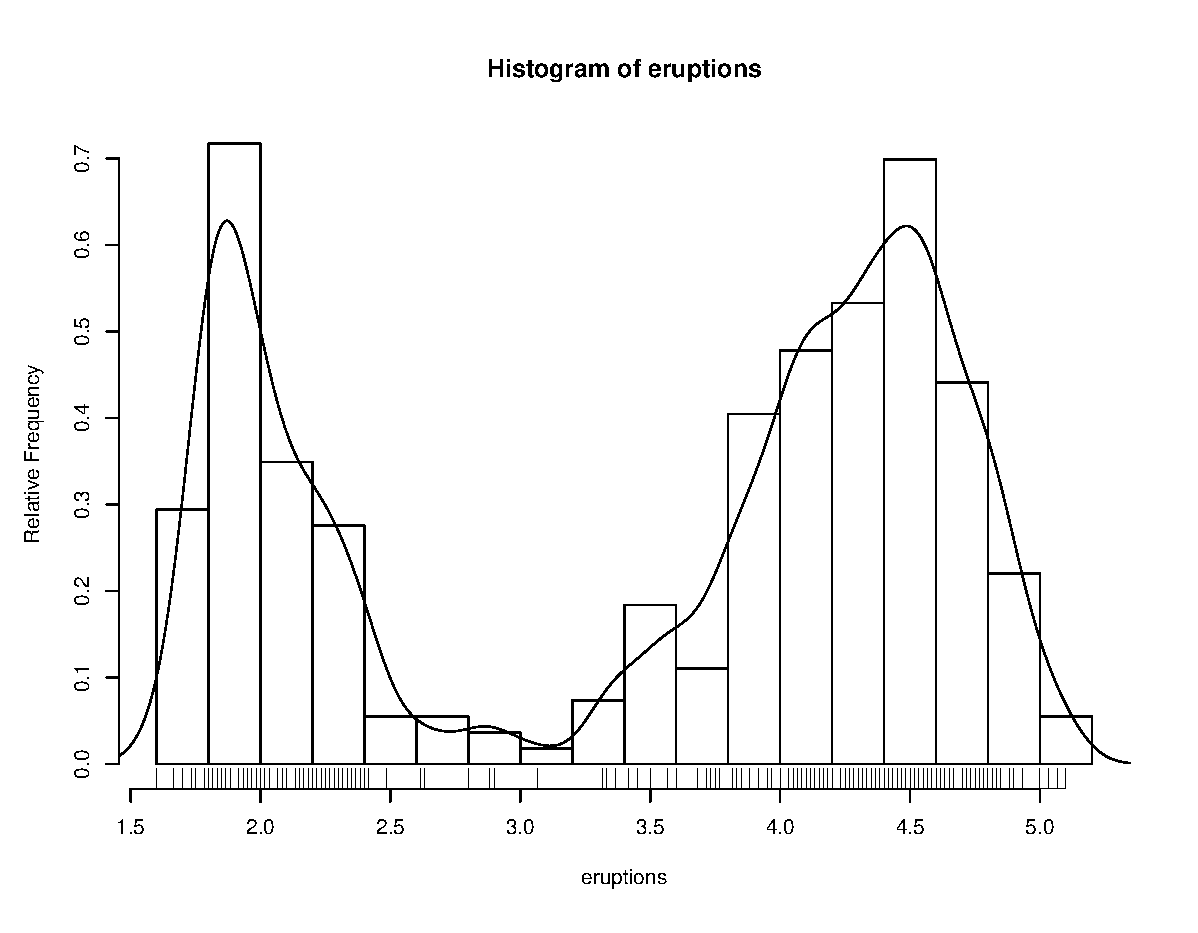
\includegraphics[width=9cm]{images/hist.eps}
\end{figure}

���ǿ����ú��� \code{ecdf} ����һ�����ݼ���
�����ۻ��ֲ���empirical cumulative distribution��
\findex{ecdf}������
\cindex{�����ۻ��ֲ�����}

\begin{example}
> plot(ecdf(eruptions), do.points=FALSE, verticals=TRUE)
\end{example}

��Ȼ������ֲ���������׼�ֲ�����ܴ�
��ô�ұߵ������ô���أ����ǻ�ɽ����3���Ӻ��״����
���ǿ������һ����̬�ֲ��������ص�ǰ��õ��ľ����ۻ��ܶȷֲ���

\begin{example}
> long <- eruptions[eruptions > 3]
> plot(ecdf(long), do.points=FALSE, verticals=TRUE)
> x <- seq(3, 5.4, 0.01)
> lines(x, pnorm(x, mean=mean(long), sd=sqrt(var(long))), lty=3)
\end{example}

\begin{figure}[h]
\centering
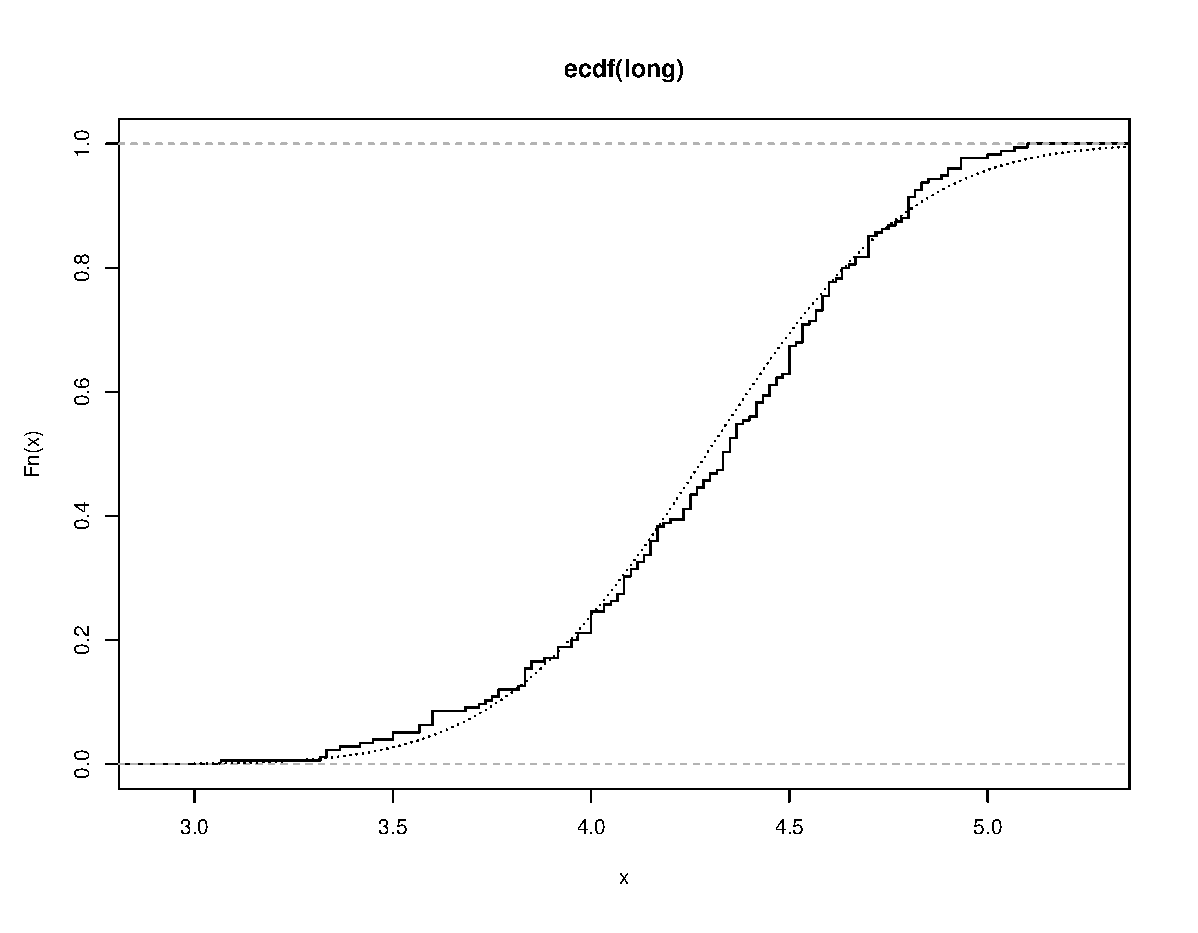
\includegraphics[width=9cm]{images/ecdf.eps}
\end{figure}

��λ�Ƚ�ͼ��Quantile-quantile (Q-Q) plot���������Ǹ�ϸ�µ��о����ߵ��Ǻϳ̶ȡ�
\cindex{��λ�Ƚ�ͼ}
\findex{qqnorm}
\findex{qqline}

\begin{example}
par(pty="s")       # ����һ�����ε�ͼ������
qqnorm(long); qqline(long)
\end{example}

\noindent
��������õ���QQͼ�������߻��DZȽ��Ǻϵģ����Ҳ�β��
ƫ����������̬�ֲ������ǿ����� \rmath{t} �ֲ�
���һЩģ���������ظ�����Ĺ���

\begin{figure}[h]
\centering
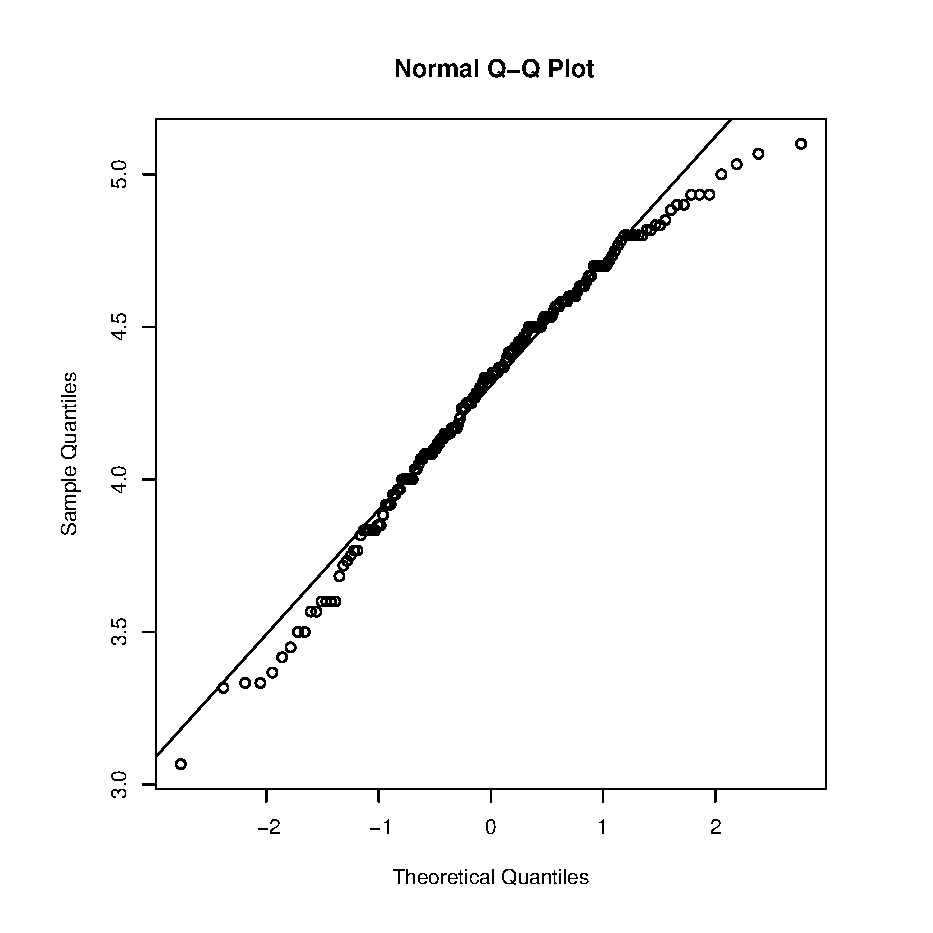
\includegraphics[width=7cm]{images/QQ.eps}
\end{figure}

\begin{example}
x <- rt(250, df = 5)
qqnorm(x); qqline(x)
\end{example}

\noindent
����õ���QQͼ���������ƫ����̬�����ij�β����(������������)��
���ǿ������������������ض��ķֲ�����Q-Qͼ

\begin{example}
qqplot(qt(ppoints(250), df = 5), x, xlab = "Q-Q plot for t dsn")
qqline(x)
\end{example}

������ǿ�����Ҫһ���Ƚ��������̬�Լ��鷽����
\R{}�ṩ�� Shapiro-Wilk ����
\cindex{Shapiro-Wilk ����}
\findex{shapiro.test}

\begin{example}
> shapiro.test(long)

         Shapiro-Wilk normality test

data:  long
W = 0.9793, p-value = 0.01052
\end{example}

\noindent
�� Kolmogorov-Smirnov ����
\cindex{Kolmogorov-Smirnov ����}
\findex{ks.test}

\begin{example}
> ks.test(long, "pnorm", mean = mean(long), sd = sqrt(var(long)))

         One-sample Kolmogorov-Smirnov test

data:  long
D = 0.0661, p-value = 0.4284
alternative hypothesis: two.sided
\end{example}

\noindent
(ע��һ���ͳ�Ʒֲ����ۣ�distribution theory�������������Ч��
��Ϊ������ͬ������������̬�ֲ��IJ�������
���Ƶġ�)

\section{��������˫��������}
\hlabel{One- and two-sample tests}
\cindex{��������˫��������}

������Ϊֹ�������Ѿ�ѧ���˵���������̬�Լ��顣
���������IJ����DZȽ�������������������
\R{} ���棬����``��ͳ''�ļ��鶼����
�� \pkg{stats} ���档������������Զ����롣

�����DZ��ڻ����̵�DZ�ȣ�latent heat��(\emph{cal/gm})
���ݣ����� Rice (1995, p.490)��

\begin{example}
Method A: 79.98 80.04 80.02 80.04 80.03 80.03 80.04 79.97
          80.05 80.03 80.02 80.00 80.02
Method B: 80.02 79.94 79.98 79.97 79.97 80.03 79.95 79.97
\end{example}

\noindent
��״ͼ��boxplot��Ϊ�����������ṩ�˼򵥵�ͼ�αȽϡ�

\begin{example}
A <- scan()
79.98 80.04 80.02 80.04 80.03 80.03 80.04 79.97
80.05 80.03 80.02 80.00 80.02

B <- scan()
80.02 79.94 79.98 79.97 79.97 80.03 79.95 79.97

boxplot(A, B)
\end{example}
\findex{boxplot}
\cindex{��״ͼ}

\noindent
��ͼ�Ͽ���ֱ�۵Ŀ�����һ������
��ȵڶ���������������ϴ��ֵ��

\begin{figure}[h]
\centering
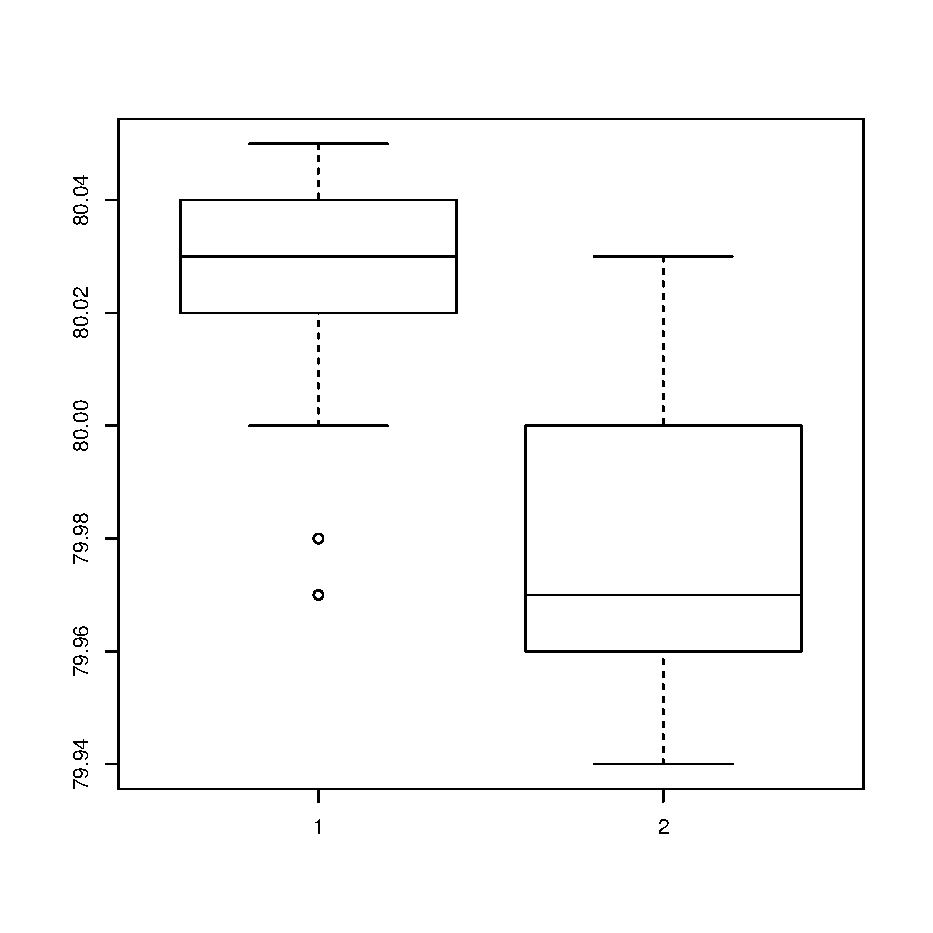
\includegraphics[width=7cm]{images/ice.eps}
\end{figure}

Ϊ�˱Ƚ����������ľ�ֵ�Ƿ���ȣ����ǿ���ʹ��
\emph{�����} \rmath{t}-����
\cindex{\rmath{t} ����}
\findex{t.test}

\begin{example}
> t.test(A, B)

         Welch Two Sample t-test

data:  A and B
t = 3.2499, df = 12.027, p-value = 0.00694
alternative hypothesis: true difference in means is not equal to 0
95 percent confidence interval:
 0.01385526 0.07018320
sample estimates:
mean of x mean of y
 80.02077  79.97875
\end{example}

\noindent
����Ľ����������̬ǰ����\footnote{����ע:\code{t}-��������̬�Լ����, �����ڽ���\code{t}-����ǰ,
ԭ������Ҫ��һ�����ݵ���̬�Լ���.}�����������Ե�ͳ�Ʋ��졣
\R{} ����Ĭ��������������룬
�� \sm{SPLUS} ���ƺ��� \code{t.test}
��Ĭ�Ϸ������ԡ����������������������̬Ⱥ�壬
���ǿ�����F������ȷ����������������

\begin{example}
> var.test(A, B)

         F test to compare two variances

data:  A and B
F = 0.5837, num df = 12, denom df =  7, p-value = 0.3938
alternative hypothesis: true ratio of variances is not equal to 1
95 percent confidence interval:
 0.1251097 2.1052687
sample estimates:
ratio of variances
         0.5837405
\end{example}
\findex{var.test}

\noindent
��������߷�����ͳ��ѧ��û���������죬���ǿ��Բ��ô�ͳ��
���跽�����Ե�\rmath{t}-���顣

\begin{example}
> t.test(A, B, var.equal=TRUE)

         Two Sample t-test

data:  A and B
t = 3.4722, df = 19, p-value = 0.002551
alternative hypothesis: true difference in means is not equal to 0
95 percent confidence interval:
 0.01669058 0.06734788
sample estimates:
mean of x mean of y
 80.02077  79.97875
\end{example}

������Щ���鶼���������ݵ���̬�ԡ�˫������
Wilcoxon (���� Mann-Whitney) ����û����̬�Ե�ǰ�ᣬ����Ҫ��
����Ч����(null hypothesis)�������������һ������������ֲ���

\cindex{Wilcoxon ����}
\findex{wilcox.test}
\begin{example}
> wilcox.test(A, B)

         Wilcoxon rank sum test with continuity correction

data:  A and B
W = 89, p-value = 0.007497
alternative hypothesis: true mu is not equal to 0

Warning message:
Cannot compute exact p-value with ties in: wilcox.test(A, B)
\end{example}

\noindent
ע�⾯����Ϣ�������������ж���ͬ������, �������Щ����������ɢ�ֲ�(�����������ݵ�
���ƴ������)��

�кö��ַ�������ͼ�λ�����ʾ���������IJ�������Ѿ�
������״ͼ�ıȽϡ����������

\begin{example}
> plot(ecdf(A), do.points=FALSE, verticals=TRUE, xlim=range(A, B))
> plot(ecdf(B), do.points=FALSE, verticals=TRUE, add=TRUE)
\end{example}

\noindent
ͬʱ��ʾ���������ľ����ۼƸ��ʷֲ����� \code{qqplot} �õ���������������
Q-Q ͼ��Kolmogorov-Smirnov �����Ƕ����������ۼƸ��ʷֲ�������ֱ����
����ͳ�Ƶġ�Kolmogorov-Smirnov ����ֻ�ٶ����ݷ���һ�������
�����ֲ���

\begin{example}
> ks.test(A, B)

         Two-sample Kolmogorov-Smirnov test

data:  A and B
D = 0.5962, p-value = 0.05919
alternative hypothesis: two.sided

Warning message:
cannot compute correct p-values with ties in: ks.test(A, B)
\end{example}
\chapter{���飬ѭ������������}
\hlabel{Loops and conditional execution}
\cindex{ѭ������������}

\section{�������ʽ}
\hlabel{Grouped expressions}
\cindex{�������ʽ}

\R{} ��һ�ֱ���ʽ���ԣ�expression language����Ϊ�����е�������ʽ
���Ƿ��ؽ���ĺ����ͱ���ʽ����ֵ����ʵ����
Ҳ��һ������ʽ������ٷ��䣬���ҿ�������
�κα���ʽ�У��������ظ�ֵ
Ҳ�������ġ�

��������ô�����Ȧ��һ�� \code{\{\var{expr\_1};
\var{\dots{}}; \var{expr\_m}\}}����ʱ����һ������Ľ��
�Ǹ��������һ�������ֵ����Ȼһ������Ȼ��һ������ʽ��
���Ϳ��ܷ��������У�����һ������ı���ʽ�У�
�ȵȡ�

\section{�������}
\hlabel{Control statements}
\cindex{�������}

\subsection{�������ƣ�\code{if}���}
\hlabel{Conditional execution}
\findex{if}

\R{} ���Ե����������ʽΪ

\examp{
> if (\var{expr_1}) \var{expr_2} else \var{expr_3}
}
\findex{if}
\findex{else}

\noindent
���� \var{expr_1} �ǿ����������Ҳ���һ��Ψһ���߼�ֵ��
����ʽ�������������Dz��Զ����ġ�

\index{f}{\verb.&&.}
\index{f}{\verb.||.}
``��·''��short-circuit�������� \code{\&\&} �� \code{||} ��������
\code{if} �����������Ʋ��֡�����Ҫע�� \code{\&}
�� \code{|} ������������������Ԫ��\footnote{����ע: ���ص�Ҳ��һ����������ȳ�������.}��
�� \code{\&\&} �� \code{||}
�����ڳ���Ϊ1�����������ұ�Ҫʱ�ŶԵڶ���������ֵ\footnote{����ע: ``��·''������һ�����ֵΪ\code{TRUE}����
\code{FALSE}����������һ��IJ����Ƿ�������.}��

\findex{ifelse}
\R{} �ṩ�� \code{if}/\code{else} �������������ʽ�ĺ���
\code{ifelse}������ʹ�÷�ʽ�� \code{ifelse(condition, a,
b)}�����շ���һ������IJ�������ͬ����������
\code{condition[i]} Ϊ��ʱ����������Ӧ��Ԫ���� \code{a[i]}������Ϊ
\code{b[i]}��


\subsection{ѭ�����ƣ�\code{for}ѭ����\code{repeat} �� \code{while}}
\hlabel{Repetitive execution}
\findex{for}

\R{} ������������ʽ�� \code{for} ѭ���ܹ�

\examp{
> for (\code{\var{name}} in \var{expr\_1}) \var{expr\_2}
}

\noindent
���� \code{\var{name}} ��ѭ��������\var{expr\_1} ��һ��
��������ʽ(������\code{1:20}������ʽ����)����
\var{expr\_2} �����Ǹ���������� \emph{name} 
����Ƶij������ʽ���� \var{name} ���� \var{expr\_1} ����
����ȡ����ֵʱ��\var{expr\_2} ����
����

�����Ǹ����ӡ��ٶ� \code{ind} �Ƿ���ָ��������vector of class indicators����
���ǽ������ַ���ָ����� \code{y} �� \code{x}��ɢ��ͼ��
һ�ַ���ʱ�ú��� \code{coplot()}\footnote{���ں����
�����������ۣ������ð� \pkg{lattice} ����ĺ���\code{xyplot}��}
������Ӧ���Ӹ���ˮƽ��ɢ��ͼ��
����һ�ַ������ǰ�����ͼ����Ļ��ͬʱ
��ʾ��������������ʾ��

\begin{example}
> xc <- split(x, ind)
> yc <- split(y, ind)
> for (i in 1:length(yc)) {
    plot(xc[[i]], yc[[i]]);
    abline(lsfit(xc[[i]], yc[[i]]))
  }
\end{example}

\findex{split}

(���� \code{split()} ͨ��ij�����Ӱ�һ��
��������ֳ�һϵ��С��������
����һ���dz����õĺ�����������
��״ͼһ��ʹ�á�����ϸ�ڿ����� \code{help} ����õ���)

\begin{quotation}
\strong{����}����������������ԣ�\R{} �����������ʹ�� 
\code{for()} ��ʽ��ѭ����䡣��~\R{} ������`��������'��whole object����ʽ
���ܼ������ָ�Ч\footnote{����ע��\R{} ������ʽ��ѭ�������ʱ��Ϳռ������Ч���ϼ����Dz������ܵġ�
����ʽ��ѭ�������ܱ���ģ����ǿ������ú�������Գ����Ԫ�ؼ���ֵ, 
����sum��mean��ͳ�ƺ�����apply��lapply ��sapply��tapply�Ⱥ��������Բ��ִ�����ʽѭ����}��
\end{quotation}

����ѭ��������

\examp{
> repeat \var{expr}
}
\findex{repeat}

\noindent
�����

\examp{
> while (\var{condition}) \var{expr}
}
\findex{while}

\noindent


�ؼ��� \code{break}�������ڽ����κ�ѭ���������Ƿdz���ġ�
���ǽ��� \code{repeat} ѭ����Ψһ�취��
\findex{break}

�ؼ��� \code{next} ������������һ���ض���ѭ����Ȼ��ֱ������
``��һ��''ѭ����
\findex{next}

��������Ӧ�ó�����
\emph{����}��ء�������һ�� \hlink{Writing your own
functions}{��д���Լ��ĺ���}�� ����ϸ���ۣ�ͬʱҲ�����ø�������ӡ�
\chapter{�����}
\hlabel{Writing your own functions}
\cindex{�����}

����ǰ����������ʾ��һ����\R{} ���������û�
�����Լ���\emph{����}��function������\R{} ��һЩ
�ڲ������������������ı���ʽ�С�ͨ��������̣�\R{} �ڳ���Ĺ����ԣ�
�����Ժ��������ϵõ�����չ��ѧд��Щ���õĺ���
��һ�������ɵش����Ե�ʹ�� \R{} ������Ҫ�ķ�ʽ��

��Ҫǿ�����ǣ��������������Ϊ
\R{} ϵͳ��һ���ֶ��ṩ����\code{mean()}, \code{var()},
\code{postscript()} �ȵȡ���Щ���������� \R{} д�ģ�
����ڱ����Ϻ��û�д��û�в��

һ��������ͨ������������ʽ����ģ�

\examp{
> name <- function(\var{arg\_1}, \var{arg\_2}, \ldots{}) \var{expression}
}
\findex{function}

\noindent
���� \var{expression} ��һ�� \R{} ����ʽ(������һ������
����ʽ)�������ò��� \var{arg_i} �������յĽ����
�ñ���ʽ��ֵ���Ǻ����ķ���ֵ��

�������κεط���
\code{\var{name}(\var{expr_1}, \var{expr_2}, \dots{})} ����ʽ���ú�����

\section{һ���򵥵�����}
\hlabel{Simple examples}

����һ���򵥵����ӣ�����������˫������
\rmath{t}-ͳ������������ʾ``�������㲽��''������һ����Ϊ�����ӣ�
��Ȼ�����������򵥵İ취�õ�һ���Ľ����

�����������£�

\begin{example}
> twosam <- function(y1, y2) {
    n1  <- length(y1); n2  <- length(y2)
    yb1 <- mean(y1);   yb2 <- mean(y2)
    s1  <- var(y1);    s2  <- var(y2)
    s <- ((n1-1)*s1 + (n2-1)*s2)/(n1+n2-2)
    tst <- (yb1 - yb2)/sqrt(s*(1/n1 + 1/n2))
    tst
  }
\end{example}

ͨ�����������������������������
ʵ��˫���� \rmath{t}-���飺

\begin{example}
> tstat <- twosam(data$male, data$female); tstat
\end{example}

�ڶ��������Ƿ�Ч
\sm{Matlab} ����ķ�б��������������������� \rmath{y}
����ͶӰ�� \rmath{X} �пռ������ϵ����
(�ⳣ������Ϊ�ع�ϵ����
��С���˷����ơ�) �������
���� \code{qr()} ��ʵ�֣�����ֱ��ʹ�����������ʱ��Ҫһ�㼼�ɡ�
�����ṩ��һ���򵥶��ְ�ȫ�ĺ�����

����һ�� \rmath{n} �� \rmath{1} ������ \rmath{y} ��һ�� \rmath{n} ��
\rmath{p} �ľ��� \rmath{X}����� \rmath{X \backslash y} ���Զ�������
$(X'X)^{-}X'y$, ���� $(X'X)^{-}$
����� \rmath{X'X}���������generalized inverse����

\begin{example}
> bslash <- function(X, y) {
  X <- qr(X)
  qr.coef(X, y)
}
\end{example}

��������󴴽����������������������У�

\begin{example}
> regcoeff <- bslash(Xmat, yvar)
\end{example}

\noindent


����� \R{} ���� \code{lsfit()} ���Ժܿ�����������ܺ�������һЩ���
������\footnote{�μ� \hlink{Statistical models
in R}{\R{}�е�ͳ��ģ��} �������ķ���}������һ���е����ֱ���ķ�ʽ
�����ú��� \code{qr()} �� \code{qr.coef()}ȥ����ⲿ�ּ��㡣
���һ���ִ��볣����ʹ�ã����ǿ��԰��ⲿ�ִ��뵥���г�����Ϊ����
ʹ�á�������������ǣ����ǿ�����������Ķ�Ԫ������binary operator��
����һ�ָ�Ϊ�����ķ�ʽ���С�

\section{�����µĶ�Ԫ������}
\hlabel{Defining new binary operators}
\cindex{��Ԫ������}

�ٶ����Ǹ��躯�� \code{bslash()} һ����ͬ�����֣�����
�������ʽ����

\examp{
\%\var{anything}\%
}

\noindent
��ô������\emph{��Ԫ������}��binary operator������ʽ�ڱ���ʽ��ʹ�ã�
�����Ǻ�������ʽ������������ \code{!}
��Ϊ�м���ַ��������������¶���

\begin{example}
> "%!%" <- function(X, y) { ... }
\end{example}

\noindent
(ע��Ҫʹ������)���ú���Ȼ��Ϳ�����
\code{X \%!\% y}����ʽʹ���ˡ�(�����ٷֺ��м���ַ���ò�Ҫ�÷�б�ܷ���
��Ϊ��ijЩ����»�����һЩ�ر�����⡣)

����ij˷������� \code{\%*\%} �����������
\code{\%o\%} ͬ�������ַ�ʽ�����
��Ԫ��������

\section{����������Ĭ��ֵ}
\hlabel{Named arguments and defaults}
\cindex{��������}
\cindex{Ĭ��ֵ}

�� \hlink{Generating regular sequences}{������������}����ʾ��һ������������ú����IJ���
��~``\code{\var{name}=\var{object}}'' ��ʽ������
���ǿ������κ�˳�����á����ǣ�������ֵ���п�����
δ�����ģ�λ�������Եķ�ʽ������ͬʱҲ�п���
����Щλ�������ԵIJ������������������ֵ��

��ˣ���������淽ʽ����ĺ��� \code{fun1}

\begin{example}
> fun1 <- function(data, data.frame, graph, limit) {
    [�������岿�ֺ���]
  }
\end{example}

\noindent
��ô�������ᱻ�ü��ַ�ʽ���ã���

\begin{example}
> ans <- fun1(d, df, TRUE, 20)
> ans <- fun1(d, df, graph=TRUE, limit=20)
> ans <- fun1(data=d, limit=20, graph=TRUE, data.frame=df)
\end{example}

\noindent
�������еķ�ʽ�ǵȼ۵ġ�

����ʱ�򣬲����ᱻ�趨һЩĬ��ֵ��
���Ĭ��ֵ�ʺ���Ҫ�������飬�����ʡ����Щ������
���磬���� \code{fun1} ������ķ�ʽ
����ʱ

\begin{example}
> fun1 <- function(data, data.frame, graph=TRUE, limit=20) { ... }
\end{example}

\noindent
�����Ա������������

\begin{example}
> ans <- fun1(d, df)
\end{example}

\noindent
���ǰ����������ȼۣ���

\begin{example}
> ans <- fun1(d, df, limit=10)
\end{example}

\noindent
�͸ı���һ��Ĭ��ֵ��

�ر�˵��һ�£�Ĭ��ֵ�������κα���ʽ�������Ǻ�������
��������������������û��Ҫ��
�dz��������ǵ����Ӳ��ó���ֻ��ʹ���������˵����

\section{\samp{\dots{}} ����}
\hlabel{The ellipsis argument (...)}

����һ�ֳ������ֵ��������Ҫ��һ�������IJ�������
���Դ��ݸ�����һ����������������ͼ�κ���ͨ�����ú��� \code{par()} 
���������� \code{plot()} �ĺ�������ͼ�β�����
\code{par()} �����Կ���ͼ�������
(�����\hlink{The par() function}{\code{par()}����} �½ڻ��������
\code{par()} ��Ϊ��ϸ�����ݡ�)�������ͨ��������
����һ������IJ�����ʵ�֡�������������Ͼ���
\samp{\dots{}}�������Ա����ݡ�
һ�������Ե����ӿ���������ʾ��

\begin{example}
fun1 <- function(data, data.frame, graph=TRUE, limit=20, ...) {
  [ʡ��һЩ���]
  if (graph)
    par(pch="*", ...)
  [ʡ���������]
}
\end{example}

\section{�ں����и�ֵ}
\hlabel{Assignment within functions}

ע��\emph{�κ��ں����ڲ�����ͨ��ֵ���Ǿֲ���
��ʱ�ģ����˳�����ʱ���ᶪʧ}�����
�����еĸ�ֵ��� \code{X <- qr(X)} ����Ӱ��
���øú����ij���ֵ�����

���Ҫ�������� \R{} ��ֵ������ԭ��
������Ҫ��Ϥ����
\emph{���}��Evalution frame���ĸ�������ڸ߼����ݣ�
���������������ۡ�

�������һ����������ȫ�ָ�ֵ�������ø�ֵ�����Բ���
``ǿ��ֵ''��superassignment�������� \code{<<-} ���߲��ú���
\code{assign()}����\code{help}������Եõ��������˵����
\sm{SPLUS} �û���Ҫע�� \code{<<-} ��
\R{} �������Ų�ͬ�����壨semantics������Щ���� \hlink{Scope}{�������÷�Χ}������ϸ���ۡ�

\section{����߼�������}
\hlabel{More advanced examples}

\subsection{��������е�Ч������}
\hlabel{Efficiency factors in block designs}

������һ���е���ﵫ��Ϊ���������ӡ���������
����һ����������е�Ч������(��������
һЩ������ \hlink{Index
arrays}{��������}���Ѿ����۹���)��

������ƣ�block design����Ҫ������������ \code{blocks} (\code{b}
��ˮƽ) �� \code{varieties} (\code{v} ��ˮƽ)�����\rmath{R} ��
\rmath{K} �ֱ��� \rmath{v} �� \rmath{v} �� \rmath{b} �� \rmath{b}
\emph{�ظ�}��replications���� \emph{�����С}��block size�������
\rmath{N} ���� \rmath{b} �� \rmath{v} ��������incidence matrix����
��ôЧ�����Ӿ���������������ֵ����
$E = I_v - R^{-1/2}N'K^{-1}NR^{-1/2} = I_v - A'A,$
���� $A = K^{-1/2}NR^{-1/2}$��
д���������һ�ַ�ʽ����

\begin{example}
> bdeff <- function(blocks, varieties) {
    blocks <- as.factor(blocks)             # minor safety move
    b <- length(levels(blocks))
    varieties <- as.factor(varieties)       # minor safety move
    v <- length(levels(varieties))
    K <- as.vector(table(blocks))           # ȥ�� dim ����
    R <- as.vector(table(varieties))        # ȥ�� dim ����
    N <- table(blocks, varieties)
    A <- 1/sqrt(K) * N * rep(1/sqrt(R), rep(b, v))
    sv <- svd(A)
    list(eff=1 - sv$d^2, blockcv=sv$u, varietycv=sv$v)
}
\end{example}

��������£�����ֵ�ֽ���������ֵ����ֵ����Ч�ʸߡ�

�����Ľ����һ���б����������Ե�һ����������ʽ������
Ч�����ӣ�������������͹淶������Ϣ��block and variety canonical contrasts����
��Ϊ��Щʱ����Щ������������õĶ�����Ϣ��

\subsection{ȥ����ӡ�����е�����}
\hlabel{Dropping all names in a printed array}

Ϊ����ʾһ�����������߾��󣬳�����Ҫ
��Ҫ��һ�������Ŀ����ʽ��ʾ��ͬʱȥ���������ͱ�š�
�򵥵�ȥ��\code{dimnames} �����Dz��ܴﵽ���Ҫ��ģ���Ϊ
\R{} ������ѿ��ַ������� \code{dimnames} ���ԡ�
Ϊ�˴�ӡһ������ \code{X}

\begin{example}
> temp <- X
> dimnames(temp) <- list(rep("", nrow(X)), rep("", ncol(X)))
> temp; rm(temp)
\end{example}

������Էdz����׵�ͨ������ĺ���
\code{no.dimnames()} ʵ�֡���������һ��``����''��wrap around��
�ķ�ʽʵ�ֵġ�������ӻ�˵��һЩ�dz���Ч���õ��û�����
�����Ƿdz����ġ�

\begin{example}
no.dimnames <- function(a) {
  ## Ϊ�˸����յĴ�ӡ���������ȥ�������е�ά������
  d <- list()
  l <- 0
  for(i in dim(a)) {
    d[[l <- l + 1]] <- rep("", i)
  }
  dimnames(a) <- d
  a
}
\end{example}

ͨ��������������������һ�ֽ��յķ�ʽ
��ʾ

\begin{example}
> no.dimnames(X)
\end{example}

��Դ����������dz����ã���Ϊ��Щ����
���ֳ�����ʽ����pattern�����ܱ����ǵ�ֵ��Ϊ��Ҫ��

\subsection{�ݹ�ʽ����ֵ����}
\hlabel{Recursive numerical integration}

���������ǵݹ�ģ������ں����ڲ������Լ���
������Ҫע����ǣ���Щ�������߱�����
���ᱻ���߲�ν�����ܣ�evaluation frame���еĺ���
���̳У���������������·����\footnote{����ע��ԭ��Ϊ``that such functions, or indeed variables,
are not inherited by called functions in higher evaluation frames as they would be if they were on
the search path.''}��

�����������ʾ��һ����򵥵�һά��ֵ���ַ�����
����������������Χ�����˺��е��ֵ�ᱻ���㡣
�����������η���one-panel trapezium rule���Ľ����
˫���(two panel) �ķdz����ƣ���ô���Ժ��߽����Ϊ����ֵ��
����ͬ���Ĺ��̻�ݹ����ڸ�����塣
����һ������Ӧ�Ļ��ֹ��̡����Ἧ�и���Զ���������������
������������ֵ\footnote{����ע��ԭ��Ϊ��``The result is an adaptive integration process
that concentrates funtion evalutions in regions where the integrand is farthest from linear.''}��
�������ַ��������е����, 
������������㷨���������ƽ������ڱ���������ƽ���ֺ�����ֵʱ��

�������ͬ�����Բ��ֵ���Ϊһ�� \R{} ��̵����������

\begin{example}
area <- function(f, a, b, eps = 1.0e-06, lim = 10) {
  fun1 <- function(f, a, b, fa, fb, a0, eps, lim, fun) {
    ## ����~`fun1'������ `����'�пɼ�
    d <- (a + b)/2
    h <- (b - a)/4
    fd <- f(d)
    a1 <- h * (fa + fd)
    a2 <- h * (fd + fb)
    if(abs(a0 - a1 - a2) < eps || lim == 0)
      return(a1 + a2)
    else {
      return(fun(f, a, d, fa, fd, a1, eps, lim - 1, fun) +
             fun(f, d, b, fd, fb, a2, eps, lim - 1, fun))
    }
  }
  fa <- f(a)
  fb <- f(b)
  a0 <- ((fa + fb) * (b - a))/2
  fun1(f, a, b, fa, fb, a0, eps, lim, fun1)
}
\end{example}

\section{������}
\hlabel{Scope}
\cindex{������}

��һ���ֵ�������Ա��ĵ��������ֵ����ݸ�ƫ��һЩ�����Ե����⡣
����������� \sm{SPLUS} �� \R{} һЩ��Ҫ�IJ��졣

�����ڲ��ı������Է�Ϊ���ࣺ
��ʽ����(formal parameters)���ֲ�����(local variables)�����ɱ���(free variables)��
��ʽ�����dz����ں����IJ����б��еı�����
���ǵ�ֵ��ʵ�ʵĺ�������
\emph{��}��ʽ�����Ĺ��̾����ġ�
�ֲ������ɺ����ڲ�����ʽ��ֵ�����ġ�
�Ȳ�����ʽ�����ֲ��Ǿֲ������ı�����
���ɱ��������ɱ����������ֵ�����ɾֲ��������۲������
�����������,

\begin{example}
f <- function(x) {
  y <- 2*x
  print(x)
  print(y)
  print(z)
}
\end{example}

����������У�\code{x} ����ʽ������\code{y} �Ǿֲ�����
��\code{z} �����ɱ�����

�� \R{} ���棬�������ú����������Ļ�����ij�������ĵ�һ�γ���
����һ�����ɱ����İ󶨡����Ϊ
\emph{�ʷ�������}��lexical scope�������ǿ��Զ���һ������ \code{cube},

\begin{example}
cube <- function(n) {
  sq <- function() n*n
  n*sq()
}
\end{example}

���� \code{sq} �еı��� \code{n} ���Ǻ����IJ�����
����������ɱ�����һЩ�������ԭ���������
ȷ��������ص�ֵ���ھ�̬������
(\sm{SPLUS})�У����ֵָ����һ����ȫ�ֱ���
\code{n} ��ص�ֵ���ڴʷ�������(\R{})�У���ָ���Ǻ���
\code{cube} �IJ�������Ϊ�� \code{sq} �����ʱ��
���ᶯ̬�󶨲��� \code{n}��
�� \R{} ����������� \sm{SPLUS} ���������ͬ������ \sm{SPLUS} ����
ȫ�ֱ��� \code{n} �� \R{}
����Ѱ�Һ���\code{cube}����ʱ�������Ļ����еı��� \code{n}��

\begin{example}
## ������ \sm{S} ����
S> cube(2)
Error in sq(): Object "n" not found
Dumped
S> n <- 3
S> cube(2)
[1] 18
## ͬ���ĺ����� \R{} �н���}
R> cube(2)
[1] 8
\end{example}

�ʻ����������躯��\emph{�ɱ�״̬}��mutable state����
�����������ʾ \R{} ���ģ��һ�����е�
�ʻ��������������ʻ�����ͬʱ�и�����֧ƽ������ܶ�ı�����
�ṩ���ҵ��ȡ��ҵ�����ʾ
��ǰ���ĺ��������ǿ����� \code{account} ����
��������������Ȼ�󷵻�һ���������ǵ�
���б��������� \code{account} ʱ��������һ����ֵ����
\code{total}�����ҷ���һ�����������������б���
��Ϊ��Щ����ʱ������һ���б���
\code{total} �Ļ����У����ǿ��Է�������ֵ��

\code{<<-} ��һ���ر�ĸ�ֵ��������������
\index{f}{\verb.<<-.}
���ĺ� \code{total} ��ص�ֵ���������������ݵ�
һ�����б�ʶ��
\code{total} ���ܱջ����С������ҵ����������
�����ò������ұߵ�ֵ�滻���������������ֵ��
�����ȫ�ֱ���������߲�εĻ�������Ȼû���ҵ���ʶ��
\code{total}����ô�ñ����ͻᱻ�������������ﱻ��ֵ��
������û��� \code{<<-} ����ȫ�ֱ��������ҰѲ������ұ�
��ֵ������\footnote{��ij����������˵��
�������е�ģ�� \sm{SPLUS} ���÷�����Ϊ�� \sm{SPLUS} �У����ֲ���������
����ȫ�ֱ������ҽ��и�ֵ������}�������� \code{<<-} ����
һ�����������������һ������������ʱ��
���������Ķ�����Ϊ�Ż���֡�

\begin{example}
open.account <- function(total) {
  list(
    deposit = function(amount) {
      if(amount <= 0)
        stop("Deposits must be positive!\n")
      total <<- total + amount
      cat(amount, "deposited.  Your balance is", total, "\n\n")
    },
    withdraw = function(amount) {
      if(amount > total)
        stop("You don't have that much money!\n")
      total <<- total - amount
      cat(amount, "withdrawn.  Your balance is", total, "\n\n")
    },
    balance = function() {
      cat("Your balance is", total, "\n\n")
    }
  )
}

ross <- open.account(100)
robert <- open.account(200)

ross$withdraw(30)
ross$balance()
robert$balance()

ross$deposit(50)
ross$balance()
ross$withdraw(500)
\end{example}

\section{���ƻ���}
\hlabel{Customizing the environment}
\cindex{���ƻ���}

�û������кü��ְ취����ʹ�û����������޸�
λ�ó�ʼ���ļ�������ÿ��Ŀ¼�������������е�һ��
��ʼ���ļ������о������ú���
\code{.First} �� \code{.Last}��

λ�ó�ʼ���ļ���·������ͨ��
�������� \env{R\_PROFILE} ���á�����ñ���û�����ã�
Ĭ����\R{}��װĿ¼�������Ŀ¼ \file{etc} �е�
\file{Rprofile.site}������ļ�������ÿ��ִ��
\R{} ʱһЩ�Զ����е�����ڶ��������ļ���
\file{.Rprofile}\footnote{��
UNIX ϵͳ�У������ļ����ɼ���}�������Է����κ�Ŀ¼���档��� \R{} �ڸ�Ŀ¼����
�����ã�����ļ��ͻᱻ���롣����ļ������û�
�������ǵĹ����ռ䣬�����ڲ�ͬ�Ĺ���Ŀ¼��
���ò�ͬ����ʼ����������ʼĿ¼��û�� \file{.Rprofile}��
\R{} �����û���Ŀ¼\footnote{����ע����~Linux ϵͳ�е�~\code{\~{}/}Ŀ¼��}��������
\file{.Rprofile} �ļ����ҵ����� (�����
���ڵĻ�)��

���������ļ����� \file{.RData} ���κν� \code{.First()} �ĺ���
 �����ض���״̬��������
\R{} �Ի���ʼʱ�Զ�ִ�в��ҳ�ʼ��������
���������еĶ�������
����ʾ����Ϊ \code{\$}���Լ������������õĶ�����
��Щ����ͬ�����������Ự�������á�

��ˣ���Щ�ļ���ִ��˳���� \file{Rprofile.site}��
\file{.Rprofile}��\file{.RData} Ȼ���� \code{.First()}�������ļ���
��������ε�ǰ���ļ��еĶ��塣

\begin{example}
> .First <- function() {
  options(prompt="$ ", continue="+\t")  # $ ����ʾ��
  options(digits=5, length=999)         # ������ֵ�������ʽ
  x11()                                 # ����ͼ�λ���
  par(pch = "+")                        # �������ݵ�ı�ʾ��
  source(file.path(Sys.getenv("HOME"), "R", "mystuff.R"))
                                        # ���˱�д�ĺ���
  library(MASS)                         # �����
}
\end{example}
\findex{.First}

���Ƶ��ǣ���������˺��� \code{.Last()}����(����)���ڶԻ�
����ʱִ�С�һ�����Ӿ���

\begin{example}
> .Last <- function() {
  graphics.off()                        # һ��С�İ�ȫ��ʩ��
  cat(paste(date(),"\nAdios\n"))        # �ó��緹�ˣ�
}
\end{example}
\findex{.Last}

\section{�࣬���ͺ������������}
\hlabel{Object orientation}
\cindex{��}
\cindex{���ͺ���}
\cindex{�������}

һ��������������������α�һ��
\emph{����}����\footnote{����ע��\R{} ���淺�κ�����Java�����
\emph{�ӿ�}(interface)��Ϊ����.����, ���������ýӿ�������������������,
���������ȷʵ����. ``���ͺ���''�ĸ������˺�ݵķ�������.}�������෴��һ�����ͺ���
��\emph{���������������}����������ض�������������ġ�
�������ȱ���κ������ԣ�
�����ڸ���������һ�����ܱ��κη��ͺ����������࣬
���ͺ�������һ��\emph{Ĭ�ϵĴ�����ʽ}��

�����һ������ʹ��������������������Ϊ�û��ṩ��Ϊ�ض�����
��ƺͱ�д���ͺ����ı��������ڶ෺�ͺ����У�\code{plot()} ����ͼ�λ���ʾ
����\code{summary()} ���ڸ������͵ĸ���������
�Լ� \code{anova()} ���ڱȽ�ͳ��ģ�͡�

�����ض���ʽ������ķ��ͺ�������Ŀ�dz��Ӵ�
���磬�����ڷdz�ʱ�ֵ������
\code{"data.frame"} ��ʹ�õĺ�����

\begin{example}
[     [[<-    any    as.matrix
[<-   mean    plot   summary
\end{example}

�����ú��� \code{methods()} �õ���ǰ��ij�������
���õķ��ͺ����б���

\begin{example}
> methods(class="data.frame")
\end{example}

�෴��һ�����ͺ������Դ�������ͬ���ܶࡣ
���磬\code{plot()} ��Ĭ�ϵķ����ͱ���
���������� \code{"data.frame"}��
\code{"density"}��\code{"factor"}���ȵȡ�һ���������б�ͬ������ͨ��
���� \code{methods()} �õ���

\begin{example}
> methods(plot)
\end{example}

���෺�κ����ĺ������岿�ַdz��Ķ̣���

\begin{example}
> coef
function (object, ...)
UseMethod("coef")
\end{example}

\noindent
~\code{UseMethod} �ij��ְ�ʾ������һ�����κ�����
Ϊ�˲鿴��Щ��������ʹ�ã����ǿ���ʹ�ú��� \code{methods()}

\begin{example}
> methods(coef)
[1] coef.aov*         coef.Arima*       coef.default*     coef.listof*
[5] coef.nls*         coef.summary.nls*

   Non-visible functions are asterisked
\end{example}

\noindent
������������������������������κ�һ�������ܼ򵥵�ͨ�������������鿴\footnote{����ע: 
����򵥵ļ�����Щ������(��\code{coef.aov}), 
\R{}�����ᱨ��������Ϣ~\code{``Error: object "coef.aov" not found''}.}��
���ǿ���ͨ���������ַ����鿴���ַ���

\findex{getAnywhere}
\findex{getS3method}
\begin{example}
> getAnywhere("coef.aov")
A single object matching 'coef.aov' was found
It was found in the following places
  registered S3 method for coef from namespace stats
  namespace:stats
with value

function (object, ...)
{
    z <- object$coef
    z[!is.na(z)]
}

> getS3method("coef", "aov")
function (object, ...)
{
    z <- object$coef
    z[!is.na(z)]
}
\end{example}

���߿��Բο��ĵ�\href{R-defs_cn.pdf}{\emph{~\R{}���Զ���}}�Եõ��������ֻ��Ƹ����������ۡ�
\chapter{R�е�ͳ��ģ��}
\hlabel{Statistical models in R}
\cindex{ͳ��ģ��}

��һ���ּٶ������Ѿ���ͳ�Ʒ������ر��ǻع�����ͷ��������һ�����˽⡣
�������ǻ���ٶ����߶Թ�������ģ�ͺͷ�����ģ��Ҳ�����˽�
\footnote{����ע: ԭ��Ϊ``Later we make some rather more ambitious presumptions, namely
that something is known about generalized linear models and nonlinear
regression.''}��

\R{} �Ѿ��ܺõض�����ͳ��ģ������е�һЩǰ�����������
�����ܹ�����һЩͨ�õķ��������ڸ������⡣

\R{} �ṩ��һϵ�н�����ϵ��ͳ��ģ����ϵĹ��ߣ�ʹ����Ϲ�����ü򵥡�
�����������������ᵽ��һ������������Ļ���
�Ǽ��ģ�����û���Ҫ����һЩ������������ȡϸ�ڵĽ����Ϣ��

\section{����ͳ��ģ�͵Ĺ�ʽ}
\hlabel{Formulae for statistical models}
\cindex{��ʽ}

����ͳ��ģ�͵�ģ����һ������
�����ķ����������ݵ�����ģ��

\[
y_i = \sum_{j=0}^p \beta_j x_{ij} + e_i,
   \qquad e_i \sim {\rm NID}(0,\sigma^2),
   \qquad i = 1, \dots{}, n
\]

�þ��������ʾ��������д��
\[
y = X \beta + e 
\]

\noindent
���� \rmath{y} ����Ӧ������\rmath{X} ��\emph{ģ��
����}��model matrix������\emph{��ƾ���}��design matrix����\rmath{X} ����
\rmath{x_0, x_1, \dots{}, x_p}��
����������determining variable����ͨ����\rmath{x_0}
�ж���1����������\emph{�ؾ�}��intercept���

\subsubsection{����}

�ڸ�����ʽ�Ķ���ǰ����һЩ�����ӿ��ܸ������˽�ȫò��

�ٶ� \code{y}, \code{x}, \code{x0}, \code{x1}, \code{x2}, \dots{} ����ֵ
������\code{X} ��һ�����󣬶�\code{A}, \code{B},
\code{C}, \dots{} �����ӡ�����������У���߸�����ʽ��
�ұ߸����ù�ʽ��ͳ��ģ�͵�������

\begin{longtable}{lp{0.68\textwidth}}
\verb.y ~ x. \\
\verb.y ~ 1 + x. &
���߶���ӳ��\rmath{y} ��
\rmath{x} �ļ�����ģ�͡���һ����ʽ������һ����ʽ�Ľؾ��
���ڶ�������һ����ʽ�Ľؾ��\\

\verb.y ~ 0 + x. \\
\verb.y ~ -1 + x. \\
\verb.y ~ x - 1. &
\rmath{y} �� \rmath{x} ��ԭ��ļ�����ģ��
(Ҳ����˵��û�нؾ���)��\\

\verb.log(y) ~ x1 + x2. &
\rmath{y} �ı任��ʽ$\log(y)$
�� \rmath{x1} �� \rmath{x2} ���еĶ��ػع� (��һ����ʽ�Ľؾ���)��\\

\verb.y ~ poly(x,2). \\
\verb.y ~ 1 + x + I(x^2). &
\rmath{y} �� \rmath{x} �Ķ��ζ���ʽ�ع顣��һ����
��������ʽ��orthogonal polynomial�����ڶ�������
ʽ��ע��������ݴΡ�\\

\verb.y ~ X + poly(x,2). &
\rmath{y} ����ģ�;���
\rmath{X} �Ͷ��ζ���ʽ��\rmath{x} ���ж��ػع顣\\

\verb.y ~ A. &
\rmath{y} �ĵ����ط������ģ�ͣ����
�� \rmath{A} ������\\

\verb.y ~ A + x. &
\rmath{y} �ĵ�����Э�������ģ�ͣ������
\rmath{A} ������Э������Ϊ \rmath{x}��\\

\verb.y ~ A*B. \\
\verb.y ~ A + B + A:B. \\
\verb.y ~ B %in% A. \\
\verb.y ~ A/B. &
\rmath{y} �� \rmath{A} �� \rmath{B}�ķǿɼ������ӷ������ģ�� ��two factor non-additive model����
ǰ������ʽ��ʾ��ͬ�Ľ��������� ��crossed classification����
��������ʽ��ʾ��ͬ��Ƕ�׷������ (nested classification)������һ��˵��
���ĸ���ʽָ��ͬһ��ģ���ӿռ䡣\\

\verb.y ~ (A + B + C)^2. \\
\verb.y ~ A*B*C - A:B:C. &
������ʵ�顣��ģ�Ͱ���һ����ЧӦ��main effects������������
�Ľ���ЧӦ ��interactions������������ʽ�ȼۡ�\\

\verb.y ~ A * x. \\
\verb.y ~ A/x. \\
\verb.y ~ A/(1 + x) - 1. &
��\rmath{A}�ĸ���ˮƽ������� \rmath{y} �� \rmath{x} �ļ����Իع顣
������ʽ�ı��벻һ�������һ����ʽ��� \rmath{A}
����ˮƽ�ֱ���ƽؾ���
��б�����\footnote{����ע��ԭ��Ϊ``Separate simple linear regression models of \rmath{y} on \rmath{x} within
the levels of \rmath{A}, with different codings.  The last form produces
explicit estimates of as many different intercepts and slopes as there
are levels in \rmath{A}.''}��\\

\verb.y ~ A*B + Error(C). &
һ��ʵ������������������� \rmath{A} �� \rmath{B}�Լ�
���� \rmath{C} ���������ֲ㣨error strata������������ʵ����ƣ�split plot experiment���У�
�������飨�����������飩��������~\rmath{C} �����ġ�\\
\end{longtable}

\index{f}{\verb.~.}
������~\code{\~} ��������~\R{} ��\emph{ģ�͹�ʽ}��model formula����
һ����ͨ������ģ�͹�ʽ���Ա�ʾΪ

\examp{
\var{response} \~{} \var{op\_1} \var{term\_1} \var{op\_2} \var{term\_2} \var{op\_3} \var{term\_3} \var{\dots{}}
}

\noindent
����
\begin{description}
\item [response]
��һ����Ϊ��Ӧ�������������߾���
������һ��ֵΪ����/����ı���ʽ��
\item [op\_i]
��һ������������Ҫô�� \code{+} Ҫô�� \code{-}���ֱ��ʾ��һ��ģ���м���
����ȥ��ijһ��(��ʽ��һ��IJ�������ѡ\footnote{����ע: ������ʡ��.}����
\item [term\_i]
����
\begin{itemize}
\item
��һ���������������ʽ����\code{1}��
\item
���ӣ�
\item
��һ�������ӣ����������ͨ��\emph{��ʽ������}
���Ӳ�����\emph{��ʽ����ʽ}��formula expression����
\end{itemize}
�����ϣ���ʽ�е��������ģ�;����е���Ҫô������Ҫô��ȥ����
\code{1} ��ʾ�ؾ������Ĭ�Ͼ��Ѽ���ģ�;��󣬳�����ʽ��ȥ����һѡ�
\end{description}

\emph{��ʽ������}��formula operators����Ч���Ϻ����ڳ��� Glim �� Genstat �е� 
Wilkinson \& Rogers ��Ƿ� (notation) ���ơ�һ�����ɱ���ĸı���
������ \samp{\code{.}} ��~\R{} ��������
\samp{\code{:}}, ��Ϊ����� \R{} �����ǺϷ��������ַ���

��Щ�����ܽ�����(�ο� Chambers \& Hastie, 1992,
p.29):

\begin{longtable}{lp{0.7\textwidth}@{}}
\code{\var{Y} \~{} \var{M}} &
\var{Y} ��ģ�� \var{M}���͡�\\

\code{\var{M\_1} + \var{M\_2}} &
ͬʱ���� \var{M\_1} �� \var{M\_2}�\\

\code{\var{M\_1} - \var{M\_2}} &
���� \var{M\_1} ���ų� \var{M\_2}�\\

\code{\var{M\_1} : \var{M\_2}} &
\var{M\_1} �� \var{M\_2} ����������tensor product���� ��������
���ӣ���ô������``����''���� (subclasses factor)\footnote{����ע�����ӽ���������}��\\

\code{\var{M\_1} \%in\% \var{M\_2}} &
�� \code{\var{M\_1}:\var{M\_2}} ���ƣ������뷽ʽ��һ����\\

\code{\var{M\_1} * \var{M\_2}} &
\code{\var{M\_1} + \var{M\_2} + \var{M\_1}:\var{M\_2}}.\\

\code{\var{M\_1} / \var{M\_2}} &
\code{\var{M\_1} + \var{M\_2} \%in\% \var{M_1}}.\\

\code{\var{M}\^{}\var{n}} &
\var{M} �����и����Լ����е�\var{n}��Ϊֹ��``��������''��
\footnote{����ע: ԭ��Ϊ��``All terms in \var{M} together with ``interactions'' up to order \var{n}''}\\

\code{I(\var{M})} &
���� \var{M}��\var{M}�����в�������һ��������������
���Ҹ��������ģ�;����С�\\
\end{longtable}

ע�⣬�ڳ���������װ����������������
�IJ���������ͨ���������㷨����͡�
\code{I()} ��һ����Ⱥ�����identity function������ʹ��
����������������������ģ�͹�ʽ�С�

��Ҫ�ر�ע��ģ�͹�ʽ����ָ����\emph{ģ�;����
����}�������˶Բ������ָ����
��ijЩ����¿��ܲ�����������
������ģ�͵IJ���ָ����

\subsection{����}
\hlabel{Contrasts}
\cindex{����}

��������Ҫ֪��ģ�͹�ʽ�����ָ��ģ�;��������ġ�
���������������DZȽϼ򵥵ģ���Ϊÿһ��������Ӧ��
ģ�;����һ����(���ģ���а����ؾ࣬
���ھ������г�ֵ����1��һ��)��

\cindex{����}
\cindex{��������}
����һ�� \rmath{k}-ˮƽ������ \code{A} ����δ����أ�������������Ӹ�����
�����Dz�һ���ġ�����\emph{����}���ӣ� ���ӵ�2��\dots{}��
�� \rmath{k} ��ͬˮƽ��ָ�����\rmath{k -
1} �С�(��������IJ������þ��ǰ�
����ˮƽ�͵�һ��ˮƽ����Ӧ�̶Ƚ��бȽ�)������
\emph{����}���ӣ�\rmath{k - 1} ����
�� \rmath{1, \dots{}, k} �ϵ������orthogonal polynomial�������Һ��Գ����

��������Ļش��е㸴�ӣ����ⲻ�������ȫ����
�����ں���һ���������ģ���к��Խؾ��
��һ��ᱻ����ָʾ��������ˮƽ�� \rmath{k} ����\footnote{����ע��
ԭ��Ϊ``First, if the intercept is omitted in a model that contains a factor
term, the first such term is encoded into \rmath{k} columns giving the
indicators for all the levels.''}��
���������Ϊ����ͨ��
\code{options} ���ò��� \code{contrasts} ���ı䡣
\R{} ��Ĭ������Ϊ

\begin{example}
options(contrasts = c("contr.treatment", "contr.poly"))
\end{example}

\noindent
����Щ���ݵ���Ҫԭ���� \R{} �� ~\sm{S} ����������
���ò�ͬ��Ĭ��ֵ��~\sm{S}���� Helmert
���ա���ˣ�������Ҫ�Ƚ���Ľ����ij�����ϻ���������
\sm{SPLUS} ����Ľ��ʱ�����������

\begin{example}
options(contrasts = c("contr.helmert", "contr.poly"))
\end{example}

\noindent
����һ���������濼�ǵĸı䡣��Ϊ�������գ�treatment contrast��(\R{}Ĭ��)
���������DZȽ���������ġ�

�⻹û�н�������Ϊ�ڸ���ģ�͵ĸ������ж��շ�ʽ������
���� \code{contrasts} �� \code{C} 
�������á�
\findex{contrasts}
\findex{C}

���ǻ�û�п��ǽ����������Щ��������������
��������ij˻�\footnote{����ע��ԭ��Ϊ``
We have not yet considered interaction terms: these generate the
products of the columns introduced for their component terms.''}��

����ϸ���Ǹ��ӵģ�\R{} �����ģ�͹�ʽ
��Ҫ����̫���׵�����¿��Բ���ͳ��ר���������ĸ���ģ�͡�
�ṩģ�͹�ʽ�ĸ�����չ��������\R{}����
���磬���ù����������ҪЧӦ��ģ�����
������������˾��ȵĽ����
������Щ����Ϊͳ��ר������Ƶġ�


\section{����ģ��}
\hlabel{Linear models}
\cindex{����ģ��}

���ڳ���Ķ���ģ�ͣ�multiple model����ϣ�������ĺ�����\code{lm()}��
�����ǵ������ķ�ʽ��һ�ָĽ��棺
\findex{lm}

\examp{
> \var{fitted.model} <- lm(\var{formula}, data = \var{data.frame})
}

����

\begin{example}
> fm2 <- lm(y ~ x1 + x2, data = production)
\end{example}

\noindent
������� \rmath{y} �� \rmath{x1} ��
\rmath{x2} �Ķ��ػع�ģ��(��һ����ʽ�Ľؾ���)��

һ����Ҫ��(�����Ͽ�ѡ)������ \code{data =
production}����ָ���κι������ģ�͵ı������ȱ�������
\emph{���ݿ�} \code{production}��
\emph{���ﲻ��Ҫ�������ݿ�
\code{production} �Ƿ񱻰�������·����}��

\section{��ȡģ����Ϣ�ķ��ͺ���}
\hlabel{Generic functions for extracting model information}

\code{lm()} �ķ���ֵ��һ��ģ����Ͻ�����󣻼����Ͼ���������
\code{"lm"} ��һ������б����������ģ�͵���Ϣ������
�ʺ϶����� \code{"lm"} �ķ��ͺ���
��ʾ����ȡ��ͼʾ�ȵȡ�
�����

\begin{example}
add1    coef       effects   kappa   predict  residuals
alias   deviance   family    labels  print    step
anova   drop1      formula   plot    proj     summary
\end{example}

����һЩ���õķ��ͺ������Լ���������¡�

\begin{longtable}{lp{0.4\textwidth}@{}}
\findex{anova}
\code{anova(\var{object\_1}, \var{object\_2})} &
�Ƚ�һ����ģ�ͺ��ⲿģ�ͣ����Ҳ�������
��������\\

\findex{coefficients}
\findex{coef}
\code{coef(\var{object})} &
��ȡ�ع�ϵ�� (����)��\\
&ȫ�ƣ�\code{coefficients(\var{object})}.\\

\findex{deviance}
\code{deviance(\var{object})} &
�в�ƽ���ͣ�����Ȩ�ؿɼ�Ȩ��\\

\findex{formula}
\code{formula(\var{object})} &
��ȡģ�͹�ʽ��Ϣ��\\

\findex{plot}
\code{plot(\var{object})} &
�����ĸ�ͼ����ʽ�в���ֵ��һЩ
���ͼ\footnote{����ע����Ҫ��������ģ���������IJв�ͼ��}��\\

\findex{predict}
\code{predict(\var{object}, newdata=\var{data.frame})} &
�ṩ�����ݿ������ͬԭʼ����һ����ǩ�ı�����
����Ƕ�Ӧ��\var{data.frame}�о�������Ԥ��ֵ��
���������\\

\code{predict.gam(\var{object},} \\
\code{newdata=\var{data.frame})} &
\code{predict.gam()} �ǰ�ȫģʽ�� \code{predict()}������������
\code{lm}, \code{glm} �� \code{gam} ��϶�����
��������ʽ��Ϊԭʼ�Ļ�����������������������ζ�ű���ʹ�ò�ͬ��ԭʼ����������\\

\findex{print}
print(\var{object}) &
��Ҫ��ӡһ����������ݡ�������ʽʹ��\footnote{����ע��һ�㲻��print()��ֱ�Ӽ��������Ҳ����������ʾ��}��\\

\findex{residuals}
\findex{resid}
\code{residuals(\var{object})} &
��ȡ�в�(����)����Ȩ��ʱ�ɼ�Ȩ��

ʡ�Է�ʽ�� \code{resid(\var{object})}��\\

\findex{step}
\code{step(\var{object})} &
ͨ�����ӻ��߼���ģ���е���ұ��������ѡ����ʵ�ģ�͡�
�������������У�AIC (Akaike ��Ϣ�淶)ֵ\footnote{����ע��\href{mailto:bnjmn_zh@yahoo.com}{Benjamin Zhao}���Ѿ�������ԭ������\texttt{step} 
���ص�Ӧ����~AIC ֵ��С��ģ�ͣ���/������������Ϊ��
\texttt {
\colorbox{exampcolor}{$>$data(swiss);}
\colorbox{exampcolor}{$>$fit $<$- lm(Fertility\~{}., data=swiss) ;}
\colorbox{exampcolor}{$>$fit.step $<$- step(fit, trace=F) ;}
\colorbox{exampcolor}{$>$AIC(fit) ;}
[1] 326.0716 
\colorbox{exampcolor}{$>$AIC(fit.step) ;}
[1] 325.2408 
}������~\texttt{fit.step} ����ģ�͵�~AIC ֵ���Բ������ֵ��
}
����ģ�ͽ��ᱻ���ء�\\

\findex{summary}
\code{summary(\var{object})} &
��ʾ����ϸ��ģ����Ͻ����\\
\end{longtable}

\section{���������ģ�ͱȽ�}
\hlabel{Analysis of variance and model comparison}
\cindex{�������}

ģ����Ϻ��� \code{aov(\code{formula},
data=\var{data.frame})}
\findex{aov}
�ͺ���
\code{lm()} �dz������ƣ���\hlink{Generic functions for extracting model information}{���ͺ�����ȡģ����Ϣ}
�����г��ķ��ͺ���ͬ�����á�

��Ҫע����� \code{aov()} ����������
������Σ�multiple error strata����ģ�ͣ�������ʵ����ƣ�split plot experiments����
������������Ϣ���е�ƽ�ⲻ��ȫ������ƣ�balanced incomplete block design���ȡ�
ģ�͹�ʽ

\examp{
\var{response} ~ \var{mean.formula} + Error(\var{strata.formula})
}
\findex{Error}

\noindent
ָ����һ������ʵ����ƣ�������\var{strata.formula} 
���塣��򵥵�����ǣ�\var{strata.formula} �ǵ����صġ�
��������һ��˫��ε�ʵ�飬Ҳ�����о�����Щ���ӵ�ˮƽ��
����ˮƽ���ʵ����Ӧ��

���磬��֪���еľ����������ӣ�ģ�͹�ʽ����
������£�

\begin{example}
> fm <- aov(yield ~ v + n*p*k + Error(farms/blocks), data=farm.data)
\end{example}

\noindent
�ⳣ����������һ��ͬʱ���о�ֵģ��
\code{v + n*p*k} ����������Σ�``ũ��֮��''��
``ũ���ڵ�������֮��''��``������''����ʵ�顣

\subsection{���������}
\hlabel{ANOVA tables}

������ķ���ʵ������Ϊ���ģ������(sequence)���е�\footnote{����ע��ԭ��Ϊ``
Note also that the analysis of variance table (or tables) are for a sequence of fitted models.''}��
��ģ�����е�\emph{�ض��ط�}����\emph{�ض�����}
��ʹ�в�ƽ���ͽ��͡�
��˽���������ʵ���У�ģ�����������
������û��Ӱ���\footnote{����ע: ԭ��Ϊ``Hence only for orthogonal experiments will the order of inclusion
be inconsequential.''}��

�ڶ��ʵ�����(multistratum experiments)�У��������Ȱ���Ӧֵ����Ͷ�䵽
����������ϣ������þ�ֵģ��ȥ��ϸ���Ͷ�䡣
ϸ�����ݿ��Բο� Chambers \& Hastie
(1992)��

����ʹ�ó���ķ����������ANOVA table����
�㻹����ֱ���ú��� \code{anova()} ���Ƚ�����ģ�͡����ַ�����Ϊ��
\findex{anova}

\examp{
> anova(\var{fitted.model.1}, \var{fitted.model.2}, \dots{})
}

�������һ���������������ʾ
���μ�������ģ�͵IJ��졣��Ҫ�Ƚϵ����ģ��
�����ǵȼ����У�hierarchical sequence���������Ĭ�ϵ�����ʵ����
û�в��ֻ��ʹ������������
�Ϳ��ơ�

\section{�������ģ��}
\hlabel{Updating fitted models}
\cindex{�������ģ��}

���� \code{update()} ��һ���dz������ĺ�����������
���һ����ԭ��ģ�����ӻ����һ�����ģ�͡�
������ʽ��
\findex{update}

\examp{
> \var{new.model} <- update(\var{old.model}, \var{new.formula})
}

�� \var{new.formula} �У���ʽ�а����ľ�㣬
\samp{\code{.}}��
\findex{.}
������ʾ``�ɵĹ�ʽģ����
�Ķ�Ӧ����''������

\begin{example}
> fm05 <- lm(y ~ x1 + x2 + x3 + x4 + x5, data = production)
> fm6  <- update(fm05, . ~ . + x6)
> smf6 <- update(fm6, sqrt(.) ~ .)
\end{example}

\noindent
�⽫�ֱ���ϴ����ݿ� \code{production} �еõ������������
���ػع�ģ�ͣ���϶�������һ��������
�����ع�����ģ�ͣ��ͽ�һ������Ӧֵ����
ƽ�����任���ģ����ϡ�

ע����� \code{data=} ���ʼ����ģ����Ϻ�����ʱ��ָ����
�����Ϣ����ͨ�����ģ�Ͷ��󴫵ݸ�
���� \code{update()} ��������ߡ�

���� \samp{.} ͬ������������������£���������
�е㲻ͬ����

\begin{example}
> fmfull <- lm(y ~ . , data = production)
\end{example}

\noindent
�����������Ӧ�� \code{y} ��
\emph{���ݿ� \code{production} �����б���}�ع��ģ�͡�

�����о��𲽻ع�ĺ�����
\code{add1()}, \code{drop1()} �� \code{step()}��
\findex{add1}
\findex{drop1}
\findex{step}
�������ϾͿ��Կ�����Щ���������壬��ϸ�ڵ����ݿ��Բο�
���߰����ĵ���

\section{��������ģ��}
\hlabel{Generalized linear models}
\cindex{��������ģ��}

�������Խ�ģ�����Խ�ģ��һ�ַ�չ����ͨ��һ�ּ�����ֱ�ӵķ�ʽʹ������ģ�ͼ��ʺ�
����̬�ֲ�����Ӧֵ�ֿ��Խ������Ա任\footnote{����ע��ԭΪΪ��
``Generalized linear modeling is a development of linear models to
accommodate both non-normal response distributions and transformations
to linearity in a clean and straightforward way.''}��
��������ģ���ǻ�������һϵ��
����ǰ��ģ�

\begin{itemize}
\item
��һ������˼����Ӧ���� \rmath{y}��һϵ�д̼�������stimulus variable��
$x_1$, $x_2$, \dots{}��
��Щ�̼�����������Ӧ���������շֲ���

\item
�̼�����\emph{����ͨ��һ�����Ժ���}Ӱ����Ӧֵ\rmath{y} �ķֲ���
�����Ժ�����Ϊ
\emph{����Ԥ����}��linear predictor��������д��
\[
\eta = \beta_1 x_1 + \beta_2 x_2 + \cdots + \beta_p x_p, 
\]
��� $x_i$ ���ҽ��� $\beta_i=0$ ʱ�� \rmath{y}�ķֲ�û��Ӱ�졣

\item
\rmath{y} �ֲ�����ʽΪ
\[
f_Y(y;\mu,\varphi)
= \exp\left[{A \over \varphi}\left\{y\lambda(\mu) -
\gamma\left(\lambda(\mu)\right)\right\} + \tau(y,\varphi)\right]
\]
���� $\varphi$ ��\emph{�߶Ȳ���}��scale parameter��(������֪)�������й۲�
�㶨��$A$ ��һ�������Ȩ�أ��ٶ�֪����
������۲ⲻͬ������ͬ��$\mu$ ��
$y$ �ľ�ֵ��
Ҳ����˵�ٶ� \rmath{y} �ķֲ�����
��ֵ��һ�����ܵij߶Ȳ��������ġ�

\item
��ֵ $\mu$ ������Ԥ������ƽ�����溯����smooth invertible function����
\[
\mu = m(\eta),\qquad \eta = m^{-1}(\mu) = \ell(\mu) 
\]
���еķ�����(inverse function) $\ell()$ ����Ϊ \emph{��������}��link function����

\end{itemize}

��Щ�ٶ��ȽϿ��ɣ����԰���ͳ��ʵ���д�������õ�ͳ��ģ�ͣ�
ͬʱҲ�㹻�Ͻ���ʹ�ÿ��Է�չ�������ƺ�ͳ������(estimation and inference)��һ�µķ�����
���ٿ��Խ���һ�£���
����������˽��ⷽ�����µĽ�չ������
�ο� McCullagh \&
Nelder (1989) ���� Dobson (1990)��

\subsection{��}
\hlabel{Families}
\cindex{��}

\R{} �ṩ��һϵ�й������Խ�ģ���ߣ�����������˵����
\emph{��˹}(gaussian), \emph{����ʽ}, \emph{����}(poisson),
\emph{���˹}(inverse gaussian) �� \emph{٤��}(gamma) ģ�͵���Ӧ�����ֲ��Լ�
��Ӧ�����ֲ�������ȷ������\emph{����Ȼ}��quasi-likelihood��ģ�͡�
�ں��ߣ�\emph{�����}��variance function��
�����ɾ�ֵ�ĺ���ָ����������������£�
�ú�����������Ӧ�����ķֲ��õ���

ÿһ����Ӧ�ֲ��������ֹ�����������ֵ������Ԥ��������������
��Щ�Զ����õĹ����������±���ʾ��

\begin{quotation}
\begin{tabbing}
xxxxxxxxxxxxxxxxxxxxxxxxx \= xxxxxxxxxxxxxxxxxxxxxxxxxxxxxxxxxxxxxxxxxxx \kill
������ \> �������� \\
\code{binomial} \> \code{logit}, \code{probit}, \code{log}, \code{cloglog} \\
\code{gaussian} \> \code{identity}, \code{log}, \code{inverse} \\
\code{Gamma} \> \code{identity}, \code{inverse}, \code{log} \\
\code{inverse.aussian} \> \code{1/mu\^{}2}, \code{identity}, \code{inverse}, \code{log} \\
\code{poisson} \> \code{identity}, \code{log}, \code{sqrt} \\
\code{quasi} \> \code{logit}, \code{probit}, \code{cloglog}, \code{identity},\\
\> \code{inverse}, \code{log}, \code{1/mu\^{}2}, \code{sqrt} 
\end{tabbing}
\end{quotation}

��Щ����ģ�͹��������е���Ӧ�ֲ������������͸���
������Ҫ����Ϣͳ��Ϊ��������ģ�͵�\emph{��}��family����

\subsection{\code{glm()}����}
\hlabel{The glm() function}
\findex{glm}

��Ȼ��Ӧ�ķֲ�\emph{����}ͨ����һ��һ�����Ժ���������
�̼���������ô��������ģ�͵Ļ���ͬ��
��������ָ��һ������ģ�͵����Բ��֡�
�����������һ�ֲ�ͬ�ķ�ʽָ����

\R{} ���ڹ������Իع�ĺ����� \code{glm()}��
����ʹ����ʽΪ

\examp{
> \var{fitted.model} <- glm(\var{formula}, family=\var{family.generator}, data=\var{data.frame})
}

�� \code{lm()} ��ȣ�Ψһ��һ�������Ծ���������IJ���\var{family.generator}��
����ʵ��һ�����������֣��������������һ�������ͱ���ʽ�б�
���ڶ���Ϳ���ģ�͵Ĺ�������ƹ���\footnote{����ע��ԭ��Ϊ: 
``The only new feature is the \var{family.generator}, which is the
instrument by which the family is described.  It is the name of a
function that generates a list of functions and expressions that
together define and control the model and estimation process.''}��
������Щ���ݿ�ʼ�������е㸴�ӣ�
�����Ƿdz�����ʹ�á�

��Щ�����DZ�׼�ġ���������������������Բμ� \hlink{Families}{��} ���ֱ�����
��``����''����ѡ��һ����������ʱ��
�ù�������������������ͬʱ������������Ϊ
�����趨���� \code{��}��quasi��
�������棬�����Ҳ�������ַ�ʽ�趨��

һЩ���ӿ��ܻ�ʹ������̸������

\subsubsection{\code{gaussian}��}

����

\begin{example}
> fm <- glm(y ~ x1 + x2, family = gaussian, data = sales)
\end{example}

\noindent
�������������һ��

\begin{example}
> fm <- lm(y ~ x1+x2, data=sales)
\end{example}

\noindent
����Ч���ϣ�ǰ�߲�һ�㡣ע�⣬��˹��û���Զ��ṩ���������趨��ѡ�
��˲��������ò�����
��һ��������Ҫ�÷DZ�׼���������ĸ�˹�壬
��ôֻ�ܲ������Ǻ������۵� 
\code{��}�塣

\subsubsection{\code{����ʽ}��}

���� Silvey (1970) �ṩ��һ�������С���ӡ�

�� Kalythos �� Aegean ���ϣ����Ծ��񳣳�����
һ��������ۿƼ��������������������������������ԡ�
�����Ѽ��˸�������ε������Ծ����������ͬʱ��¼��ä�۵���Ŀ��
����չʾ���£�

\begin{quotation}
\begin{tabbing}
xxxxxxxxxxxxx \= xxx \= xxx \= xxx \= xxx \= xxx \kill
Age:          \>  20 \>  35 \>  45 \>  55 \>  70 \\
No.: tested: \>  50 \>  50 \>  50 \>  50 \>  50 \\
No.: blind:  \>  \w{ 6} \>  17 \>  26 \>  37 \>  44 \\
\end{tabbing}
\end{quotation}

������֪��������Щ�����Ƿ��Ǻ� logistic �� probit ģ�ͣ�
���ҷֱ���Ƹ���ģ�͵� LD50��Ҳ����һ�����Ծ���ä�۵ĸ���
Ϊ50\%ʱ������䡣

��� \rmath{y} �� \rmath{n} �ֱ�������Ϊ \rmath{x} ʱ��ä����Ŀ�ͼ��
������Ŀ������ģ�͵���ʽ��Ϊ
$$ y \sim {\rm B}(n, F(\beta_0 + \beta_1 x)) $$
������ probit ģ���У�
$F(z) = \Phi(z)$
�DZ�׼����̬�ֲ����������� logit ģ��
(Ĭ��)�У�
$F(z) = e^z/(1+e^z)$��
������ģ���У�
$$ \hbox{LD50} = -\beta_0/\beta_1 $$
�����ֲ������IJ���Ϊ0ʱ���ڵĵ㡣

��һ���ǰ�����ת�������ݿ�,

\begin{example}
> kalythos <- data.frame(x = c(20,35,45,55,70), n = rep(50,5),
                         y = c(6,17,26,37,44))
\end{example}

�� \code{glm()} ��϶���ʽģ��ʱ����Ӧ����
�����ֿ����ԣ�

\begin{itemize}
\item
�����Ӧ������\emph{����}�� ��ٶ�����\emph{��Ԫ}��binary��
���ݣ����Ҫ����\rmath{0/1}������

\item
�����Ӧ������\emph{˫�о���}����ٶ���һ��
Ϊ����ɹ��Ĵ����ڶ���
Ϊ����ʧ�ܵĴ�����

\item
�����Ӧ������\emph{����}�����һˮƽ��Ϊʧ��
(0) ���Ƕ���������Ϊ`�ɹ�'(1) ���ǡ�
\end{itemize}

������Dz��õ��ǵڶ��ֹ��������������ݿ���
������һ������

\begin{example}
> kalythos$Ymat <- cbind(kalythos$y, kalythos$n - kalythos$y)
\end{example}

Ϊ�������Щģ�ͣ����Dz���

\begin{example}
> fmp <- glm(Ymat ~ x, family = binomial(link=probit), data = kalythos)
> fml <- glm(Ymat ~ x, family = binomial, data = kalythos)
\end{example}

��Ȼ logit �Ĺ���������Ĭ�ϵģ�������ǿ����ڵڶ���������ʡ�Ըò�����
Ϊ�˲鿴��Ͻ��������ʹ��

\begin{example}
> summary(fmp)
> summary(fml)
\end{example}

����ģ�Ͷ���ϵĺܺá�Ϊ�˼��� LD50�����ǿ���
����һ���򵥵ĺ�����

\begin{example}
> ld50 <- function(b) -b[1]/b[2]
> ldp <- ld50(coef(fmp)); ldl <- ld50(coef(fml)); c(ldp, ldl)
\end{example}

����Щ�����еõ�������ֱ���43.663���
43.601�ꡣ

\subsubsection{Poisson ģ��}

Poisson ��Ĭ�ϵĹ��������� \code{log}����ʵ�ʲ����У�
��һ�峣��������ϼ������ϵ� Poisson ��������ģ�͡�
��Щ�������ϵ�ʵ�ʷֲ��������϶���ʽ�ֲ���
����һ���dz���Ҫ�����Ӵ�Ļ��⣬���Dz�������������չ����
�������Ƿ�-��˹����ģ�����ݵ���Ҫ���֡�

��ʱ��ʵ���в����� Poisson �����ڶ�������ƽ����
ת����ɵ�����̬���ݴ�����
��Ϊ���ߵ���һ��ѡ���ǣ�һ��
Poisson ��������ģ�Ϳ���ͨ������ķ�ʽ��ϣ�

\begin{example}
> fmod <- glm(y ~ A + B + x, family = poisson(link=sqrt),
              data = worm.counts)
\end{example}

\subsubsection{����Ȼģ��}

�������е��壬��Ӧ�����ķ��������ھ�ֵ����ӵ��
��Ϊ������multiplier���ij߶Ȳ�����
����Ծ�ֵ��������ʽ����Ӧ�ֲ���һ�����ԣ�
�������poisson�ֲ�
$\hbox{Var}[y] = \mu$��

��������Ȼ���ƺ��ƶϣ����Dz����趨��ȷ����Ӧ�ֲ�����
�趨���������ͷ��������ʽ����Ϊ���������ͷ�����������ھ�ֵ��
��Ȼ����Ȼ���ƺ� gaussian �ֲ�ʹ�õļ����dz����ƣ�
�����һ��˳���ṩ��һ���÷DZ�׼�����������߷����
���gaussianģ�͵ķ�����

���磬���Ƿ����Իع�����
$$ y = {\theta_1z_1 \over z_2 - \theta_2} + e $$
ͬ��������д��
$$ y = {1 \over \beta_1x_1 + \beta_2x_2} + e $$
����
$x_1 = z_2/z_1$, $x_2=-1/x_1$, $\beta_1=1/\theta_1$ and
$\beta_2=\theta_2/\theta_1$��
�������ʺϵ����ݿ����ǿ�������
����������

\begin{example}
> nlfit <- glm(y ~ x1 + x2 - 1,
               family = quasi(link=inverse, variance=constant),
               data = biochem)
\end{example}

�����Ҫ�Ļ������߿��Դ������ֲ�
���߰����ĵ��еõ��������Ϣ��

\section{��������С���˷��������Ȼ��ģ��}
\hlabel{Nonlinear least squares and maximum likelihood models}
\cindex{��������С���˷�}

�ض���ʽ�ķ�����ģ�Ϳ���ͨ����������ģ��
(\code{glm()}) ��ϡ���������ʱ�����DZ���ѷ�������ϵ�����
��Ϊһ���������Ż�����������\R{}�ķ������Ż������� \code{optim()}��
\code{nlm()} �� \code{nlminb()}����\R{}2.2.0��ʼ����
\findex{nlm}
\findex{optim}
���߷ֱ��滻 \sm{SPLUS} �� \code{ms()} �� \code{nlminb()}�����ܸ�ǿ��
����ͨ����Ѱ����ֵʹ��ȱ���ȣ�lack-of-fit��ָ����ͣ���
\code{nlm()} ����ͨ��ѭ�����Ը��ֲ���ֵ�õ�����ֵ��
�����Իع鲻ͬ������һ����������һ���ȶ�ֵ��
\code{nlm()} ��Ҫ�趨���������ij�ʼֵ��
�����������Ƿ������ںܴ�̶���������
��ʼֵ���õ�����\footnote{����ע: ������һЩ����ķ����жϳ�ʼ�IJ����趨��}��

\subsection{��С���˷�}
\hlabel{Least squares}

��Ϸ�����ģ�͵�һ�ְ취����ʹ���ƽ���ͣ�SSE����в�ƽ������С��
����۲⵽��������̬�ֲ������ַ����Ƿdz���Ч�ġ�

�������������� Bates \& Watts (1988)��51ҳ�����������ǣ�

\begin{example}
> x <- c(0.02, 0.02, 0.06, 0.06, 0.11, 0.11, 0.22, 0.22, 0.56, 0.56,
         1.10, 1.10)
> y <- c(76, 47, 97, 107, 123, 139, 159, 152, 191, 201, 207, 200)
\end{example}

����ϵ�ģ���ǣ�

\begin{example}
> fn <- function(p) sum((y - (p[1] * x)/(p[2] + x))^2)
\end{example}

Ϊ�˽�����ϣ�������Ҫ���Ʋ�����ʼֵ��һ��Ѱ��
������ʼֵ�İ취������ͼ�λ���Ȼ�����һЩ����ֵ��
����������Щֵ��������ģ�����ߡ�

\begin{example}
> plot(x, y)
> xfit <- seq(.02, 1.1, .05)
> yfit <- 200 * xfit/(0.1 + xfit)
> lines(spline(xfit, yfit))
\end{example}

��Ȼ�����ǿ������ĸ��ã����dz�ʼֵ 200 �� 0.1 Ӧ���㹻�ˡ�
��������ϣ�

\begin{example}
> out <- nlm(fn, p = c(200, 0.1), hessian = TRUE)
\end{example}
\findex{nlm}

��Ϻ�\code{out\$minimum} ������ƽ���ͣ�SSE����
\code{out\$estimate} �Dz�������С���˹���ֵ��
Ϊ�˵õ��������ƹ����н��Ƶı�׼��(SE)�����ǿ��ԣ�

\begin{example}
> sqrt(diag(2*out$minimum/(length(y) - 2) * solve(out$hessian)))
\end{example}

���������е�2��ʾ�����ĸ�����һ��95\%
���Ŷ��������ͨ�� $\pm$ 1.96
SE ����õ������ǿ��԰������С����������߻���
һ���µ�ͼ�ϣ�

\begin{example}
> plot(x, y)
> xfit <- seq(.02, 1.1, .05)
> yfit <- 212.68384222 * xfit/(0.06412146 + xfit)
> lines(spline(xfit, yfit))
\end{example}

��׼�� \pkg{stats} �ṩ����������С���˷�
��Ϸ�����ģ�͵����乤�ߡ����Ǹո���Ϲ���ģ����
Michaelis-Menten ģ�ͣ���˿����������������õ����ƵĽ��ۡ�

\begin{example}
> df <- data.frame(x=x, y=y)
> fit <- nls(y ~ SSmicmen(x, Vm, K), df)
> fit
Nonlinear regression model
  model:  y ~ SSmicmen(x, Vm, K)
   data:  df
          Vm            K
212.68370711   0.06412123
 residual sum-of-squares:  1195.449
> summary(fit)

Formula: y ~ SSmicmen(x, Vm, K)

Parameters:
    Estimate Std. Error t value Pr(>|t|)
Vm 2.127e+02  6.947e+00  30.615 3.24e-11
K  6.412e-02  8.281e-03   7.743 1.57e-05

Residual standard error: 10.93 on 10 degrees of freedom

Correlation of Parameter Estimates:
      Vm
K 0.7651
\end{example}

\subsection{�����Ȼ��}
\hlabel{Maximum likelihood}
\cindex{�����Ȼ��}

�����Ȼ����Maximum likelihood��Ҳ��һ�ַ�������Ϸ�������������������
������̬�������С����ַ������ƵIJ���
����ʹ�ö�����Ȼֵ�����߸��Ķ�����Ȼֵ
����������������� Dobson (1990), pp. :
108--111��������ӶԼ�������Ӧ������� logisticģ��
����ȻҲ������ \code{glm()} ��ϣ��������ǣ�

\begin{example}
> x <- c(1.6907, 1.7242, 1.7552, 1.7842, 1.8113,
         1.8369, 1.8610, 1.8839)
> y <- c( 6, 13, 18, 28, 52, 53, 61, 60)
> n <- c(59, 60, 62, 56, 63, 59, 62, 60)
\end{example}

Ҫʹ��������Ȼֵ��С����

\begin{example}
> fn <- function(p)
   sum( - (y*(p[1]+p[2]*x) - n*log(1+exp(p[1]+p[2]*x))
           + log(choose(n, y)) ))
\end{example}

\noindent
����ѡ��һ���ʵ��ij�ʼֵ����ʼ��ϣ�

\begin{example}
> out <- nlm(fn, p = c(-50,20), hessian = TRUE)
\end{example}
\findex{nlm}

\noindent
��Ϻ�\code{out\$minimum} ���Ǹ�������Ȼֵ��
\code{out\$estimate} ���������Ȼ��ϵIJ���ֵ��
Ϊ�˵õ���Ϲ��̽��Ƶı�׼�����ǿ��ԣ�

\begin{example}
> sqrt(diag(solve(out$hessian)))
\end{example}

�������Ƶ� 95\% �Ŷ��ڼ���� \code{����ֵ} $\pm$
1.96 SE ����õ���

\section{һЩ�DZ�׼ģ��}
\hlabel{Some non-standard models}

�ڽ�������ǰ�����Ǽ���һ�� \R{} ����ijЩ����ijЩ����ع��
���ݷ�������Ĺ��ߡ�

\begin{itemize}
\item
\cindex{���ģ��}
\strong{���ģ�ͣ�Mixed models����}�û����װ� \pkg{nlme} �����ṩ��
���� \code{lme()} �� \code{nlme()}��
\findex{lme}
\findex{nlme}
��Щ�����������ڻ��ЧӦģ�ͣ�mixed-effects models�������Ժͷ����Իع顣Ҳ����˵
�����Ժͷ����Իع��У�һЩϵ����������ص�Ӱ�졣
��Щ������Ҫ������ù�ʽ������ģ�͡�

\item
\cindex{�ֲ����ƻع�}
\strong{�ֲ����ƻع�(Local approximating regressions)��}���� \code{loess()}
\findex{loess}
���þֲ���Ȩ�ع����һ���Dz����ع顣
���ֻع����ʾһ���������ݵ����ƺ�
���������ݼ�����������dz����á�

���� \code{loess} ��ͶӰ���ٻع飨projection pursuit regression���Ĵ���
һ����ڱ�׼�� \pkg{stats} �С�
\findex{loess}

\item
\cindex{�Ƚ��ع�}
\strong{�Ƚ��ع�(Robust regression)��}�ж��������������
��ϻع�ģ�ͣ�ͬʱ��������������
����ֵ��Ӱ�졣���Ƽ��� \pkg{MASS} �еĺ��� \code{lqs}
\findex{lqs}
Ϊ���Ƚ��Ե�����ṩ�����µ��㷨�����⣬�Ƚ��Խϵ͵�ͳ��ѧ�ϸ�Ч�ķ���
ͬ�������ڰ� \pkg{MASS} �еõ���
�纯��
\code{rlm}��
\findex{rlm}

\item
\cindex{�ۼ�ģ��}
\strong{�ۼ�ģ��(Additive models)��}���ּ�����������ͨ������������
ƽ���ۼӺ�����smooth additive function�������ع麯����һ����˵��ÿ����������
����һ��ƽ���ۼӺ������û����׵İ� \pkg{acepack} ����ĺ��� \code{avas} ��
\code{ace}
\findex{avas}
\findex{ace}
�Լ��� \pkg{mda} ����ĺ��� \code{bruto} �� \code{mars}
\findex{bruto}
\findex{mars}
Ϊ���ּ����ṩ��һЩ���ӡ�
���ּ�����һ���������û����װ� 
\pkg{gam} �� \pkg{mgcv} ����ʵ��
��\strong{�����ۼ�ģ��}��

\item
\cindex{����ģ��}
\strong{����ģ��(Tree-based models)��}�����������ڵ�ȫ������ģ��
Ԥ��ͽ������ݣ���������������ģ�͵ݹ���ھ����Ա������жϵ��Ͻ�
���ݵķֲ�ֿ�������������������շֳɼ�����ͬ�飬ʹ��
���ھ��������ƶ���価���ܲ��졣
����������õ�һЩ�������ݷ�����������
�����ĵ���Ϣ��

ģ�Ϳ�����һ�������ģ����ʽָ������ģ����Ϻ���
�� \code{tree()}��
\findex{tree}
�������෺�ͺ������� \code{plot()} �� \code{text()}
�����Ժܺõ���������ģ����Ͻ����ͼ����ʾ��

\R{} ���������ģ�ͺ�������\emph{ͨ��}�û����׵İ�
\pkg{rpart} �� \pkg{tree} �õ���

\end{itemize}

\include{graphics}
\chapter{��}
\cindex{��}
\hlabel{Packages}

���е� \R{} ���������ݼ��DZ�����\emph{��}��packages������ġ�ֻ�е�һ��
��������ʱ���������ݲſ��Ա����ʡ�������һ��Ϊ�˸�Ч
(�������б����ȥ�������ڴ沢������������ʱ��)��
һ��Ϊ�˰������Ŀ����߷�ֹ���������������е����ֳ�ͻ��
������������
\href{R-exts_cn.pdf}{��д\R{}����չ}��������ϸ�Ľ��ܡ�������ǽ������û��ĽǶ���
����������⡣

����ʹ�����������鿴�㵱ǰ�����а�װ�İ�

\begin{example}
> library()
\end{example}

\noindent
������û�в�����Ϊ������ij���ر�İ�(��� \pkg{boot}
�����а����ĺ������� Davison \& Hinkley (1997))��ʹ��
��������

\begin{example}
> library(boot)
\end{example}

�û�����ʹ�ú��� \code{CRAN.packages()}
���������� (Ҳ����ͨ�� Windows �� RAqua ͼ�ν����ϵ� \code{Packages} �˵�����)
�����������Զ����ºͰ�װ����

Ϊ�˲鿴��ǰ����Щ�������ˣ�������

\begin{example}
> search()
\end{example}

\noindent
���������б�����һЩ�б���Ȼ�����뵫����
�����������б���(\hlink{Namespaces}{�����ռ�})��

Ϊ�˲鿴�Ѿ���װ�İ������п��Է��ʵİ��������б���
����ʹ��

\begin{example}
> help.start()
\end{example}

\noindent
�⽫����һ�� \HTML{} ��ʽ�İ���ϵͳ��Ȼ��ͨ��
\code{Reference} �������ӵ����а����б��� 

\section{��׼��}
\hlabel{Standard packages}

��׼(\emph{����})������ \R{} ԭ�����һ����Ҫ���֡�
���ǰ������� \R{} �����ĵĻ����������ͱ��ĵ���������
���ݼ�����׼ͳ�ƺ�ͼ�ι��ߡ�
���κ� \R{} �İ�װ�汾�У����Ƕ��ᱻ�Զ���á�
��\href{R-FAQ_cn.pdf}{\R{}�������⼯}������Եõ�һ���������б���

\section{���װ��� \acronym{CRAN}}
\cindex{CRAN}
\hlabel{Contributed packages and CRAN}

������ص�����Ϊ \R{} �����˺ü��ٸ�����
����һЩ��ʵ�����ض���ͳ�Ʒ���������һЩ
�������ݺ�Ӳ���ķ��ʽӿڣ�������
��Ϊ�̿���IJ�����ϡ�һЩ��(\emph{�Ƽ�}
��)�Ͷ�������ʽ�� \R{} ���󷢲�������Ŀ��Դ�
\textbf{CRAN}
(\url{http://CRAN.R-project.org/} �����ľ���)������һЩ
��Դ���� Bioconductor (\url{http://www.bioconductor.org/}) ���صõ���
\emph{\R{}�������⼯} ����һ���Ѿ����������б���
�������Եõ��İ����嵥����Ƿdz�Ѹ�ٵġ�

\section{�����ռ�}
\cindex{�����ռ�}
\findex{::}
\findex{:::}
\hlabel{Namespaces}

�����Լ���\emph{�����ռ�}��namespaces���������������л����ĺ��Ƽ���
�İ��������ڰ� \code{datasets}�������ռ���Ҫ�������ã�
�������������������غ��������ݣ���ֻ�����ڲ��û�ʹ�ã�
���Ƿ�ֹ������һ���û����������������ߣ�ʹ��
��ͬ����ʱ���ƻ��������ṩ��һ��
�����ض�����ij������ķ�����

���磬\code{t()} �� \R{} �����ת�ú����������û�
���ܻᶨ��һ�������� \code{t}�������ռ�
��ֹ�û�����ĺ������Ⱥ��ƻ�
����ת�õĺ�����

�������������������ռ���ء�˫ð�Ų�����
\code{::} ѡ��һ���ض������ռ�õ��ĺ������塣
������������У�ת�ú������ǿ���ͨ��
\code{base::t} ʹ�ã���Ϊ�����ڰ� \code{base} �ж���ġ�
һ�����еĺ�������ͨ�����ַ�ʽ���ʡ�

��ð�Ų����� \code{:::} ���ܻ������һЩ \R{} �����У�
���е���˫ð�Ų������������Է������ض���
�û�������ʹ�ú��� \code{getAnywhere()}��
�����������ذ���

�������ǰ�֮�������ģ�inter-dependent������������һ�����ܻ�����������
���Զ����롣�����ᵽ��ð�Ų�����ͬ��������
��ذ����Զ����롣���������ռ�İ��Զ�����ʱ��
���Dz��ᱻ�Զ�����
�������


%\chapter{������������}
\label{test biosino 1}
�ؼ�\footnote{����һ��}�ǵ���multindDGH��\cindex{������}

\begin{description}
\item[\rc{-e}]
\item[\rc{--example}]{
����˵��
}
\item[\rc{ --t.t}]{
	����
}

\end{description}

\section{���Խ�}
\label{cs dgh}
\begin{figure}
\includegraphics{figures/test.ps}
\caption{This is caption of figure}
\end{figure}

���Ӳ��Ե� \ref{test biosino 1} ��;

\pagebreak

���Խ�\ref{cs dgh}��\pageref{cs dgh}
������\key{ESC};

\r{}


\backmatter
\chapter{��¼1 һ����ʾ�Ự}
\hlabel{A sample session}

����ĻỰ\footnote{����ע: ������������Linux������д�ġ�������~Windows �û�Ӱ�첻��}
�����ڲ����ж�
\R{} ������һЩ�����и��򵥵��˽⡣���ϵͳ���������Կ�ʼʱ����
�е㲻��Ϥ�����󣬵���Щ�Ի��ܿ�
��ʧ�ġ�

��¼�������������ϵͳ��

\begin{example}
$ R
\end{example}

���ʵ��ķ�ʽ���� \R{}\footnote{����ע��Windows �û�ֱ�ӵ�� R �Ŀ��ͼ����롣������ Windows ����һ��������}�� 

\R{} ����ʼ��������һ�������

(�� \R{} ���棬��ߵ���ʾ�������ᱻ��ʾ��ֹ
������)

\examp{help.start()}\\
���� \HTML{} ��ʽ�����߰���(ʹ����ļ��������
���õ������)������������
�����������ӡ�

��С���������ڣ�������һ���֡�

\begin{example}
x <- rnorm(50)
y <- rnorm(x)
\end{example}
��������α��̬��������� \rmath{x} ��
\rmath{y}��

\examp{plot(x, y)} \\
����άɢ��ͼ��һ��ͼ�δ��ڻ��Զ����֡�

\examp{ls()} \\
�鿴��ǰ�����ռ������ \R{} ����

\examp{rm(x, y)} \\
ȥ��������Ҫ�Ķ���(���)��

\examp{x <- 1:20} \\
�ȼ��� \rmath{x = (1, 2, \dots{}, 20)}��

\examp{w <- 1 + sqrt(x)/2} \\
��׼���`Ȩ��'������

\begin{example}
dummy <- data.frame(x=x, y= x + rnorm(x)*w)
dummy
\end{example}
����һ����\rmath{x} �� \rmath{y}���ɵ�˫��\emph{���ݿ�}��
�鿴���ǡ�

\begin{example}
fm <- lm(y ~ x, data=dummy)
summary(fm)
\end{example}
��� \rmath{y} �� \rmath{x} �ļ����Իع飬�鿴
���������

\begin{example}
fm1 <- lm(y ~ x, data=dummy, weight=1/w^2)
summary(fm1)
\end{example}
���������Ѿ�֪����׼���һ����Ȩ�ع顣

\examp{attach(dummy)} \\
�����ݿ��е����������һ��ı�������ʹ�á�

\examp{lrf <- lowess(x, y)} \\
��һ���Dzξֲ��ع顣

\examp{plot(x, y)} \\
��׼ɢ��ͼ��

\examp{lines(x, lrf\$y)} \\
���Ӿֲ��ع����ߡ�

\examp{abline(0, 1, lty=3)} \\
�����Ļع����ߣ�(�ؾ� 0��б�� 1)��

\examp{abline(coef(fm))} \\
��Ȩ�ػع����ߡ�

\examp{abline(coef(fm1), col = "red")} \\
��Ȩ�ع����ߡ�

\examp{detach()} \\
�����ݿ������·����ȥ����

\begin{example}
plot(fitted(fm), resid(fm),
	 xlab="Fitted values",
	 ylab="Residuals",
	 main="Residuals vs Fitted")
\end{example}
һ�������췽���ԣ�heteroscedasticity���ı�׼�ع����ͼ��
����Կ�����

\examp{qqnorm(resid(fm), main="Residuals Rankit Plot")} \\
����̬��ֵͼ�������ݵ�ƫ�ȣ�skewness������ȣ�kurtosis�����쳣ֵ��outlier����
������û�ж�����;��ֻ����ʾһ�¶��ѡ���

\examp{rm(fm, fm1, lrf, x, dummy)} \\
�ٴ���ա�

�ڶ����ֽ��о�
Michaelson �� Morley �������ٵľ���ʵ�顣������ݼ�����
�Ӷ��� \code{morley} �еõ����������Ǵ��ж�����������ʾ
���� \code{read.table} �����á�

\begin{example}
filepath <- system.file("data", "morley.tab" , package="datasets")
filepath
\end{example}
�õ��ļ�·����

\examp{file.show(filepath)} \\
��ѡ���鿴�ļ����ݡ�

\begin{example}
mm <- read.table(filepath)
mm
\end{example}
�����ݿ����ʽ��ȡ Michaelson �� Morley �����ݣ����Ҳ鿴��
���������ʵ��(\code{Expt} ��)��ÿ������ 20 ��
(\code{Run} ��)�Ĺ۲�õ������ݿ��е� \code{sl} �ǹ��ٵļ�¼��
��Щ�������ʵ���ʽ���롣

\begin{example}
mm$Expt <- factor(mm$Expt)
mm$Run <- factor(mm$Run)
\end{example}
�� \code{Expt} �� \code{Run} ��Ϊ���ӡ�

\examp{attach(mm)} \\
��������λ�� 3 (Ĭ��) �ɼ���������ֱ�ӷ��ʣ���

\examp{plot(Expt, Speed, main="Speed of Light Data", xlab="Experiment No.")} \\
�ü򵥵ĺ�״ͼ�Ƚ����ʵ�顣

\begin{example}
fm <- aov(Speed ~ Run + Expt, data=mm)
summary(fm)
\end{example}
����������飬`runs' �� `experiments' ��Ϊ���ӡ�

\begin{example}
fm0 <- update(fm, . ~ . - Run)
anova(fm0, fm)
\end{example}
��Ϻ��� `runs' ����ģ�ͣ����Ҷ�ģ�͸���ǰ��
����������

\begin{example}
detach()
rm(fm, fm0)
\end{example}
�ڽ������湤��ǰ��������ݡ�

�������ڲ鿴����Ȥ��ͼ����ʾ���ԣ��ȸ��ߺ�Ӱ����ʾ��

\begin{example}
x <- seq(-pi, pi, len=50)
y <- x
\end{example}
\rmath{x} ��һ����
$-\pi\leq x \leq \pi$ �ڵȼ���50��Ԫ�ص�������
\rmath{y} ���ơ�

\begin{example}
f <- outer(x, y, function(x, y) cos(y)/(1 + x^2))
\end{example}
\rmath{f} ��һ���������зֱ� \rmath{x}
�� \rmath{y} ��������Ӧ��ֵ�Ǻ���
$\cos(y)/(1 + x^2)$ �Ľ����

\begin{example}
oldpar <- par(no.readonly = TRUE)
par(pty="s")
\end{example}
����ͼ�β������趨ͼ������Ϊ``������''��

\begin{example}
contour(x, y, f)
contour(x, y, f, nlevels=15, add=TRUE)
\end{example}
���� \rmath{f} �ĵȸ��ߣ�����һЩ������ʾϸ�ڡ�

\examp{fa <- (f-t(f))/2} \\
\code{fa} �� \rmath{f} ��``�ǶԳƲ���''(\code{t()} ��ת��
����)��

\examp{contour(x, y, fa, nlevels=15)} \\
���ȸ��ߣ�\dots{}

\examp{par(oldpar)}\\
\dots{} �ָ�ԭʼ��ͼ�β�����

\begin{example}
image(x, y, f)
image(x, y, fa)
\end{example}
����һЩ���ܶȵ�Ӱ����ʾ��(�������Ҫ������Ա���
����Ӳ����)�� \dots{}

\examp{objects(); rm(x, y, f, fa)}\\
\dots{} �ڼ�����һ��ǰ��������ݡ�

\R{} �������������㡣

\begin{example}
th <- seq(-pi, pi, len=100)
z <- exp(1i*th)
\end{example}
\code{1i} ��ʾ���� \rmath{i}��

\begin{example}
par(pty="s")
plot(z, type="l")
\end{example}
ͼ�β����Ǹ���ʱ����ʾ�鲿��ʵ����ͼ���������
һ��Բ��

\examp{w <- rnorm(100) + rnorm(100)*1i}\\
�ٶ������������Բ�������������һ�ַ���
���ø������鲿��ʵ��ֵ�DZ�׼��̬���
�� \dots{}

\examp{w <- ifelse(Mod(w) > 1, 1/w, w)} \\
\dots{} ��Բ��ĵ�ӳ������ǵĵ�����

\begin{example}
plot(w, xlim=c(-1,1), ylim=c(-1,1), pch="+",xlab="x", ylab="y")
lines(z)
\end{example}
���еĵ㶼��Բ�У����ֲ�����
���ȵġ�

\begin{example}
w <- sqrt(runif(100))*exp(2*pi*runif(100)*1i)
plot(w, xlim=c(-1,1), ylim=c(-1,1), pch="+", xlab="x", ylab="y")
lines(z)
\end{example}
�ڶ��ַ������þ��ȷֲ�������Բ���еĵ�
����ȥ���ȶ��ˡ�

\examp{rm(th, w, z)} \\
�ٴ���ա�

\examp{q()}\\
�뿪 \R{} ��������ܱ���ʾ�Ƿ񱣴� \R{} �����ռ䣬
��������һ�������ԵĻỰ������ܲ���
��������

\chapter{��¼2 ���� R}
\hlabel{Invoking R}

\section{ ��������� R}
\hlabel{Invoking R from the command line}

�� UNIX ���� Windows ������ģʽ�²���ʱ��
���� \samp{R} �������������ʽ
������ \R{} ��������

\examp{
\code{R} [\var{options}] [\code{<}\var{infile}] [\code{>}\var{outfile}],
}

\noindent
���ǻ�����ͨ�� \code{R CMD} �ӿ����������ýӿ��Ǹ��ֲ��뱻``ֱ��''���ʵ� 
(�磬���� \R{} �ĵ���ʽ���ļ�����
�����������ȥ�İ�) \R{} ���ߵ�һ�ְ�װ��

�� UNIX ���棬��Ҫȷ�Ż�������
\env{TMPDIR} ��û�����û�������ָ����һ��������·����
������ʱ�ļ���Ŀ¼��

�����ѡ������������һ�� 
\R{} �Ự����ʼ����ֹʱ�������������ƽ�������������(�鿴�����ĵ���
���� \samp{Startup} �����⣬���������
��һЩ Windows-�����ϸ��)��

\begin{itemize}
\item
���Ǹ��� \code{--no-environ}��\R{} �����Զ������û���λ���ļ�
�����û���������λ���ļ�����
���ɻ�������
\env{R\_ENVIRON} ָ���ģ������û���趨��Ĭ����\\
\texttt{\$R\_HOME/etc/Renviron.site}
(���������)���û��ļ����ڵ�ǰ�����û���Ŀ¼����� \file{.Renviron}��
��Щ�ļ�����
�� \samp{\var{name}=\var{value}} ��ʽ��ֵ����
(\code{help(Startup)} ���Եõ���׼ȷ������)�������趨��
�������ܻ����� \env{R\_PAPERSIZE} (Ĭ�ϵ�ҳ������/��С)��
\env{R\_PRINTCMD} (Ĭ�ϵĴ�ӡ����) �� \env{R\_LIBS} (ָ��
�������Ӱ� \R{} ��������б�)��

\item
\R{} ����λ�ù㷺���������������ļ����������Ѿ������������ѡ��
\code{--no-site-file}�������ļ������ֿ���ͨ��
�������� \env{R\_PROFILE} ���ʡ����
�ñ���û�����ã�����ʹ��Ĭ�ϵ��ļ� \file{\$R\_HOME/etc/Rprofile.site}
����������ڣ���

\item
Ȼ�󣬳��� \code{--no-init-file} ���趨��\R{} ������������ǰĿ¼�����û���Ŀ¼
һ���� \file{.Rprofile} ���ļ�
Ȼ����������

\item
����� \file{.RData} �ļ��������ᱻ����(����ָ��
\code{--no-restore} ���� \code{--no-restore-data})��

\item
������ \code{.First} ���ڣ���Ҳ�ᱻִ�С�
�������(�� \R{} �Ի�����ʱ���е� \code{.Last} Ҳһ��)
�������ʵ������������ļ��ж��壬����
�����ļ� \file{.RData} �С�
\end{itemize}

���⣬�п�ѡ�����
\R{} ���̵��ڴ�ʹ����� (�ο����߰������� \samp{Memory} ������
)���û�һ������õ���Щ���ã�������
���þ� \R{} �������ڴ档

\R{} �������µ������ѡ�

\begin{longtable}{lp{0.68\textwidth}}
\code{--help} \\
\code{-h} &
���׼�����ӡ��̵İ�����Ϣ����˳���˳���\\

\code{--version} &
���׼�����ӡ�汾��Ϣ����˳���˳��� \\

\code{--encoding=\var{enc}} &
�Կ���̨����
\code{stdin} ������ָ�����뷽ʽ�� ��� \code{iconv} ���ƣ�
�鿴���İ����ļ���\\

\code{RHOME} &
���׼�����ӡ \R{} ��``��Ŀ¼''����˳���˳���
������ shell �ű��� man ҳ��
\R{} ��װ�����л�����ж��� (ִ���ļ��������ȵ�)
���������Ŀ¼�¡�\\

\code{--save} \\
\code{--no-save} &
���� \R{} �Ự����ʱ�Ƿ񱣴����ݼ���
�����һ�ν���ʽ�Ự�У����߶�û�и�������ô
���û����� \kbd{q()} �˳�ʱ����Ҫ������Ƿ񱣴����ݣ�
�ڷǽ���ʽ����ʱ������һ�ַ�ʽҪ���趨�� \\

\code{--no-environ} &
����ȡ�κ��û��ļ�ȥ�趨���������� \\

\code{--no-site-file} &
����ʱ����ȡ�κ�λ���ļ��� \\

\code{--no-init-file} &
����ʱ����ȡ�κ��û������ļ��� \\

\code{--restore} \\
\code{--no-restore} \\
\code{--no-restore-data} &
�����Ƿ�������ʱ�ָ������ļ�(ָ���� \R{} ����ʱĿ¼�µ��ļ� \file{.RData})��
Ĭ����
�ָ��� (\code{--no-restore} ��ʾ����ָ���Ŀ�ѡ��
\code{--no-restore-*}��)\\

\code{--no-restore-history} &
�����Ƿ�������ʱ�ָ���ʷ�ļ�(������ \R{} ����Ŀ¼�µ��ļ� \file{.Rhistory}��
����ͨ����������
\env{R\_HISTFILE} �����趨)��Ĭ����
�ָ���\\

\code{--vanilla} &
ͬʱ�趨�� \code{--no-save}, \code{--no-environ}
\code{--no-site-file}, \code{--no-init-file} �� \code{--no-restore}�� \\

\code{--no-readline} &
(������ UNIX) ��ֹͨ�� \strong{readline} ���������б༭�����
�� Emacs ���� \sm{ESS} (``Emacs
Speaks Statistics'') ������ \R{} �dz����á���\hlink{The command-line editor}{�����б༭��}���� 
���Եõ��������Ϣ�� \\

\code{--ess} &
(������ Windows)ͨ�� \code{R-inferior-mode} ģʽ�� \sm{ESS} ������ \code{Rterm}�� \\

\code{--min-vsize=\var{N}} \\
\code{--max-vsize=\var{N}} &
ͨ���趨``������ջ''��vector heap����СΪ \var{N} �ֽڣ�
ָ���ɱ��С�����������С�ڴ�ռ������
\var{N} Ҫô��һ��������Ҫô���Էֱ��ʾ `Giga' (2\^{}30)��`Mega' (2\^{}20)��
`Kilo' (2\^{}10�������)����`kilo' (1000����׼)�� \samp{G}��
\samp{M}��\samp{K} �� \samp{k}���������\\

\code{--min-nsize=\var{N}} \\
\code{--max-nsize=\var{N}} &
ͨ���趨``cons ��Ԫ''��cons cells������ĿΪ \var{N}�� 
ָ�������С�����������С�ڴ�ռ������
�ο�ǰ����� \var{N} ��ϸ�����ݡ���32λ�����棬һ�� cons ��Ԫ����28���ֽڣ�
����64λ�����棬������ 56 ���ֽڡ�\\

\code{--max-ppsize=\var{N}} &
�趨ָ�뱣��ջ������СΪ \var{N}
��λ�㡣Ĭ��ֵΪ 10000����ʱ��Ҫ���Ӹ�ֵ����Ӧ
��ĸ��Ӽ��㡣��������������趨ֵΪ
100000��\\

\code{--max-mem-size=\var{N}} &
(�������� Windows) �趨���� \R{} ����͹����ռ��ڴ��������޶ȡ�
Ĭ������Ϊ
1024Mb �ͻ����ϵ������ڴ棬����СҪ����
16Mb��\\

\code{--quiet} \\
\code{--silent} \\
\code{-q} &
����ʾ��ʼ�İ�Ȩ�ͻ�ӭ��Ϣ�� \\

\code{--slave} &
�� \R{} ������ƽ�������С���ѡ������
֧������ \R{} �����Ϊ����ij��� \\

\code{--verbose} &
�� \R{} ѡ��
\code{verbose} �趨Ϊ \code{TRUE}ʱ����ʾ���й����и������Ϣ��\R{} ʹ�����ѡ��
���������Ϣ������� \\

\code{--debugger=\var{name}} \\
\code{-d \var{name}} &
(������ UNIX) ͨ�������� \var{name} ���� \R{}��ע������������£���һ��������
�п�ѡ��ᱻ���ԣ�����������
\R{} ���ڲ���������ʼִ��ʱ������ \\

\code{--gui=\var{type}} \\
\code{-g \var{type}} &
(������ UNIX) ʹ�� \var{type} ��Ϊ�û�ͼ�νӿ�(ע����Ҳ����
����ʽͼ�νӿ�)�����ڣ���������
\var{type} ��ֵ�� \samp{X11}��Ĭ�ϣ��ٶ��Ѿ���װ \samp{Tcl/Tk}����
 \samp{Tk}��\samp{gnome}���ٶ�
\acronym{GNOME} �Ѿ���װ���� \samp{none}��\\

\code{--args} &
�����ǻ���ʣ��������к��ԣ�
�������
\code{commandArgs()} �õ�����ֵ�dz������á� \\
\end{longtable}

ע�⣬�����ó���ķ���(��
\samp{$<$} �� \samp{$>$}) �ض���������������� Windows 9X/ME ϵͳ������ʹ�����Ϣ�ᱻ����
��׼������Ϣ�� (\code{stderr})��

���� \code{R CMD} �������ø��ֿ�������
\R{} �IJ���``ֱ��''���ʵĹ��ߡ�
һ�����ʽΪ

\examp{
R CMD \var{command} \var{args}
}

\noindent
���� \var{command} �ǹ�������\var{args} �Ǵ��ݸ���
�IJ�����

���ڣ�����Ĺ��߿��Ե���

\begin{longtable}{lp{0.72\textwidth}}
\code{BATCH} &
������ģʽ���� \R{}��\\
\code{COMPILE} &
(������ UNIX)�� \R{} �����ļ��� \\
\code{SHLIB} &
Ϊ��̬���봴�������⣨shared library����\\
\code{INSTALL} &
��װ�������ӵİ��� \\
\code{REMOVE} &
ȥ���������ӵİ��� \\
\code{build} &
����(Ҳ���Ǵ��)�������ӵİ���\\
\code{check} &
ѡ��������ӵİ��� \\
\code{LINK} &
(������ UNIX)������ִ�г����ǰ�ˡ� \\
\code{Rprof} &
\R{} �ĺ�����Post-process�������ļ��� \\
\code{Rdconv} &
�� Rd ��ʽת���ɸ���������ʽ������ \HTML{}��Nroff��
\LaTeX{}�����ı��� \sm{S} �ĵ���ʽ��\\
\code{Rd2dvi} &
�� Rd ��ʽת���� DVI/PDF ��ʽ�� \\
\code{Rd2txt} &
�� Rd ��ʽת�����ı���ʽ�� \\
\code{Sd2Rd} &
�� S �ļ�ת���� Rd ��ʽ�� \\
\code{config} &
(������ UNIX) ���������Ϣ��\\
\end{longtable}

ʹ��

\begin{example}
R CMD \var{command} --help
\end{example}

\noindent
��ÿ����� \code{R CMD} �ӿڷ��ʵĹ���
��ʹ����Ϣ��

\section{ �� Windows �µ��� R}
\hlabel{Invoking R under Windows}

�����ַ��������� Windows ������ \R{}�����ն˴���
(��\code{cmd.exe}��\code{command.com}������������ǿ�Ľű�)����
���� \code{R.exe} ���߸�ֱ�ӵ� \code{Rterm.exe}ʱ��ǰ��
�ᵽ�ķ������ܶ�����ʹ��������Ҫ����
������)�����ڽ���ʽ�û�������ʹ�û��ڿ���̨��ͼ�ν���
(\code{Rgui.exe})��

�� Windows ������������̺� UNIX �еĹ��̷dz����ƣ�
���DZ���ָ��`��Ŀ¼'��home directory������Ϊ
Windows ϵͳ���ᶨ�����Ŀ¼����������˻������� \env{R\_USER}��
���Ŀ¼���������ָ�����������������������
\env{HOME} �����ˣ���Ҳ��ָ����Ŀ¼��ͨ���������û��ɿص����ã�
\R{} ���������ҵ��û�����ĸ�Ŀ¼��
�����Ȳ��� Windows ϵͳ��"˽��"Ŀ¼
(���͵�˽��Ŀ¼�� Windows XP ϵͳ�е� 
\code{C:$\backslash$Documents and Settings$\backslash$username$\backslash$My Documents}
)������������ɹ�����
�������� \env{HOMEDRIVE} �� \env{HOMEPATH} ���趨��
(���dz������� Windows NT/2000/XP ϵͳ�¶���)����Щ���������Ŀ¼��
�����Щ��û���趨����ô�Ͱ�
��ʼĿ¼���ɸ�Ŀ¼��

�������������� \samp{\var{name}=\var{value}} ��ʽ
���������е�β����

����������п�ѡ����
���� \code{RGui.exe} ʱ���á�

\begin{longtable}{lp{0.68\textwidth}}
\code{--mdi} \\
\code{--sdi} \\
\code{--no-mdi} &
������ MDI ����(Ĭ�ϣ�
��һ���������п������ж���Ӵ���)����SDI ����
(ͼ�Σ�ҳ��Ϳ���̨�Ķ��ظ߲�δ���)����ʽ���� \code{Rgui}��\\

\code{--debug} &
���� \code{Rgui} �IJ˵���``Break to debugger''���ã����ҿ���
�������д������趨�ϵ㡣 \\
\end{longtable}

�� Windows ϵͳ�У�������� \code{R CMD} ������ָ���� \file{*.bat}
�� \file{*.exe} ������Ҫ�ڲ����
����Ļ���������������������У�
\env{R\_HOME}��\env{R\_VERSION}��\env{R\_CMD}��\env{R\_OSTYPE}��\env{PATH}��
\env{PERL5LIB}���� \env{TEXINPUTS}�����磬��������õ�·������
\file{latex.exe}����ô

\begin{example}
R CMD latex.exe mydoc
\end{example}
\noindent
���� \file{mydoc.tex} ���� \LaTeX{} ���Ұ� \R{} ��
\file{share/texmf} ���·���ӵ��������� \env{TEXINPUTS} �С�

\section{ �� Mac OS X �µ��� R}
\hlabel{Invoking R under Mac OS X}

�� Mac OS X �������� \R{} �����ַ�ʽ���� Terminal.app ���ڵ���
\code{R} ʱ��ǰ���ᵽ�ķ��������á�
ͬ�����л��ڿ���̨��ͼ�ν��� (\code{R.app})����Ĭ�ϰ�װ��
ϵͳ�� \code{Applications} �ļ����С�
����һ����׼��˫�������� Mac OS X ����

Mac OS X ���������̺� UNIX �µ����̷dz����ơ�
`��Ŀ¼'�� R.framework �����á�����Ŀ¼�͵�ǰĿ¼
����Ϊ�û��ĸ�Ŀ¼����Ȼ�������
��ͼ�ν����еIJ���ѡ�񴰿��������趨һ��
��ͬ������Ŀ¼��

\chapter{��¼3 �����б༭��}
\hlabel{The command-line editor}

\section{Ԥ������}

������ UNIX ϵͳ�Ѿ���װ�� \acronym{GNU} \strong{readline} �⣬
��ô \R{} ������������ UNIX �±��� \R{} ���룬�������õ�
�����б༭�����༭�����µ�����ǰ�ù������
ע�⣺�ø�¼�ᵽ�Ľӿ�\strong{����}���� UNIX ϵͳ��
\acronym{GNOME}�ӿڣ����������ڱ�׼��������
�ӿڡ�

�������ʱ�����˲��� \code{--no-readline} (ʹ�� \acronym{ESS} ʱ�dz�����\footnote{
`Emacs Speaks Statistics' �����μ� \acronym{URL}
\url{http://ESS.R-project.org}})�� 
���������á�

Windows �汾�� \R{} �м򵥵������б༭���ܣ�
�� \acronym{GUI} ����� \samp{Help} �˵��µ� \samp{Console}���Ѿ�
���� \code{Rterm.exe} �����������
�ļ� \file{README.Rterm}��

��ʹ�� \strong{readline} д \R{} ����ʱ������
�����ĺ������á�

��Щ���������ǿ����ַ�������Ԫ�ַ���Meta character���������ַ�����
\kbd{Control-m} ��ʾͬʱ��ס
\key{CTRL} �� \key{m} ����������
\kbd{C-m} ��ʽ��ʾ��Ԫ�ַ����� \kbd{Meta-b} ��ʾͬʱ��ס
\key{META}\footnote{�� PC �����ϣ���������
Alt ����ż����`Windows'����} �� \key{b} ����������
\kbd{M-b} ��ʽ��¼���������ն�û��
\key{META} ����������� \kbd{ESC} ��ʼ�������ַ�����
����Ԫ�ַ�����˶��� \kbd{M-b}������Լ���
\key{ESC}\key{b}��\kbd{ESC} �ַ�������
������Ԫ�����ն�Ҳ�������ġ�ע���������
��Ԫ�ַ�����������ġ�

\section{�༭}

\R{} ���������������е���ʷ��
��������������ʷ�ļ��е�������Ա����µ��ã��޸�
���µ��������ʽ�����ύ����
Emacs-��ʽ�������б༭�У��κ�ֱ�ӵ�����
���Ὣ�ַ�ֱ�Ӳ��뵽�����༭�������У�
����ȡ������Ҳ���ַ���
\emph{vi} ����ģʽ��ͨ�� \kbd{M-i} ��
\kbd{M-a} �������ַ����Ա����벢��ͨ������
\key{ESC} ��������ģʽ��

�κ�ʱ����� \key{RET} ����ʹ������
���±��ύ��

�����ı༭����������ı��������ܽᡣ

\section{�����б༭�ܽ�}

\textbf{���µ�������ʹ�ֱ�ƶ�}

\begin{longtable}{lp{0.68\textwidth}}
\code{C-p} &
����ǰһ������(������ʷ�ļ�)��\\
\code{C-n} &
������һ������(ǰ����ʷ�ļ�)��\\
\code{C-r \var{text}} &
���������ַ��� \var{text} �����һ����� \\
\end{longtable}

�ڴ�����նˣ������ʹ�����¼��ֱ����
\kbd{C-p} �� \kbd{C-n}��

\textbf{ˮƽ�ƶ�ָ��}

\begin{longtable}{lp{0.68\textwidth}}
\code{C-a} &
�ص������п�ͷ�� \\
\code{C-e} &
������������� \\
\code{M-b} &
����һ�����ʡ� \\
\code{M-f} &
ǰ��һ�����ʡ� \\
\code{C-b} &
����һ���ַ��� \\
\code{C-f} &
ǰ��һ���ַ��� \\
\end{longtable}

�ڴ�����նˣ������ʹ�����Ҽ��ֱ����
\kbd{C-b} �� \kbd{C-f}��

\textbf{�༭�����ύ}

\begin{longtable}{lp{0.68\textwidth}}
\code{\var{text}} & 
�ڹ�괦�����ı� \var{text}�� \\
\code{C-f \var{text}} &
�ڹ������ \var{text}�� \\
\code{\key{DEL}} &
ɾ��ǰ����ַ�(������)�� \\
\code{C-d} &
ɾ����괦���ַ��� \\
\code{M-d} &
ɾ����괦��������IJ��֣�����``����''���ǡ� \\
\code{C-k} &
ɾ����굽��������IJ��֣�����``����''���ǡ� \\
\code{C-y} &
�������``����''���ı��� \\
\code{C-t} &
ת�ù�괦���ı��� \\
\code{M-l} & 
���ַ�ת����Сд�ַ��� \\
\code{M-c} &
������ת���ɴ�д�� \\
\code{\key{RET}} &
������ \R{} �ύ��� \\
\end{longtable}

���� \key{RET} �������ֹ�����б༭��

\printindex{c}{��¼4 ��������}
\printindex{f}{��¼5 ��������}
\chapter{��¼6 �ο�����}
\hlabel{References}

\noindent
D.~M.~Bates and  D.~G.~Watts (1988), \emph{Nonlinear Regression
Analysis and Its Applications.} John Wiley \& Sons, New York.

\noindent
Richard A.~Becker, John M.~Chambers and Allan R.~Wilks (1988),
\emph{The New S Language.} Chapman \& Hall, New York.
This book is often called the ``\emph{Blue Book}''.

\noindent
John M.~Chambers and Trevor J.~Hastie eds. (1992),
\emph{Statistical Models in S.} Chapman \& Hall, New York.
This is also called the ``\emph{White Book}''.

\noindent
John M.~Chambers (1998)
\emph{Programming with Data}. Springer, New York.
This is also called the ``\emph{Green Book}''.

\noindent
A.~C.~Davison and D.~V.~Hinkley (1997), \emph{Bootstrap Methods
and Their Applications}, Cambridge University Press.

\noindent
Annette J.~Dobson (1990), \emph{An Introduction to Generalized Linear
Models}, Chapman and Hall, London.

\noindent
Peter McCullagh and John A.~Nelder (1989), \emph{Generalized Linear
Models.} Second edition, Chapman and Hall, London.

\noindent
John A. Rice (1995), \emph{Mathematical Statistics and Data Analysis.}
Second edition.  Duxbury Press, Belmont, CA.

\noindent
S.~D.~Silvey (1970), \emph{Statistical Inference.} Penguin, London.
%%%%%%%%%%%%%%%%%%%%%%%%%%%%%%%%%%%%%%%%%%%%%%%%%%%%%%%%%%%%%%%%%%
% Contents: Who contributed to this Document
% $Id: contrib.tex,v 1.2 2002/05/26 22:44:33 zuohuijun Exp $
%%%%%%%%%%%%%%%%%%%%%%%%%%%%%%%%%%%%%%%%%%%%%%%%%%%%%%%%%%%%%%%%%
\chapter{���}
\hlabel{A sample session}
%\noindent Much of the material used in this introduction comes from an
%Austrian introduction to \LaTeX\ 2.09 written in German by:
\noindent ����ݽ�����ʹ�õ������������һ���µ�����ʹ�õ���׫д\footnote{����ע���Ҳ�ϲ������}
��~\LaTeX\ 2.09���ܣ�
\begin{verse}
\contrib{Hubert Partl}{partl@mail.boku.ac.at}%
{Zentraler Informatikdienst der Universit\"at f\"ur Bodenkultur Wien}
\contrib{Irene Hyna}{Irene.Hyna@bmwf.ac.at}%
   {Bundesministerium f\"ur Wissenschaft und Forschung Wien}
\contrib{Elisabeth Schlegl}{no email}%
   {in Graz}
\end{verse}

%If you are interested in the German document, you can find a version
%updated for \LaTeXe{} by J\"org Knappen at\\
%\texttt{CTAN:/tex-archive/info/lshort/german}
�����Ե����ĵ�����Ȥ��������ҵ�һ���� J\"org Knappen ���~\LaTeXe{}
���µİ汾����CTAN��λ���ǣ�\\
\texttt{CTAN:/tex-archive/info/lshort/german}

\vspace{\stretch{1}}
%\noindent While preparing this document, I asked
%for reviewers on \texttt{comp.text.tex}. I got a lot of response. The
%following individuals helped with corrections, suggestions and
%material to improve this paper. They put in a big effort to help me
%get this document into its present shape. I would like to
%sincerely thank all of them. Naturally, all the mistakes you'll find
%in this book are mine. If you ever find a word which is spelled
%correctly, it must have been one of the people below dropping me a
%line.
\noindent ��׼������ĵ�ʱ������\texttt{comp.text.tex}�е�ר���ǽ���
��ѯ���ҵõ��˴����Ļ�Ӧ��������˰���������У����������ṩ�Ľ����ϡ�
���Ǹ����˼������������ҽ�����ĵ�ʵ�ֳ�����������ӡ��Ҷ�����������
��ʾ���ĵĸ�л����Ȼ�أ����ڱ������ҵ������д������ҵ�ʧ������
���ҵ�ÿһ��ƴд��ȷ�ĵ��ʣ���һ���������г�����Щ��֮һ������һ�ѵĽ����

\begin{quote}
\flushleft\small
Rosemary~Bailey,        %r.a.bailey@qmw.ac.uk 0.2
Friedemann~Brauer,      %fbrauer@is.dal.ca 3.4
Jan~Busa,               % <busaj@ccsun.tuke.sk>
Markus~Br\"uhwiler,     % <m.br@switzerland.org>
David~Carlisle,         %GONE carlisle@cs.man.ac.uk 1.0
Jos\'e~Carlos~Santos,   % <jcsantos@fc.up.pt>
Mike~Chapman,           %chapman@eeh.ee.ethz.ch 3.16
Christopher~Chin,       %chris.chin@rmit.edu.au 3.1
Carl~Cerecke,           %cdc@cosc.canterbury.ac.nz>
Chris~McCormack,        %GONE chrismc@eecs.umich.edu 0.1
Wim~van~Dam,            %GONE wimvdam@cs.kun.nl 2.2
Jan~Dittberner,         %jan@jan-dittberner.de 3.15
Michael~John~Downes,    %<mjd@ams.org> 14 Oct 1999
David~Dureisseix,       %dureisse@lmt.ens-cachan.fr 1.1
Elliot,                 %GONE enh-a@minster.york.ac.uk 1.1
David~Frey,             %david@eos.lugs.ch 2.2
Robin~Fairbairns,       %Robin.Fairbairns@cl.cam.ac.uk 0.2 1.0
J\"org|~Fischer,        %j.fischer@xpoint.at 3.16
Erik~Frisk,             %frisk@isy.liu.se 3.4
Frank,                  %frank@freezone.co.uk 11 Feb 2000
Kasper~B.~Graversen,    % <kbg@dkik.dk>
Alexandre~Guimond,      %guimond@IRO.UMontreal.CA 0.9
Cyril~Goutte,           %goutte@ei.dtu.dk 2.1 2.2
Greg~Gamble,            %gregg@maths.uwa.edu.au 2.2
Neil~Hammond,           %nfh@dmu.ac.uk 0.3
Rasmus~Borup~Hansen,    %GONE rbhfamos@math.ku.dk 0.2 0.9 0.91 0.92 1.9.9
Joseph~Hilferty,        % <hilferty@fil.ub.es>
Bj\"orn Hvittfeldt,     %bjorn@hvittfeldt.com 3.13
Martien~Hulsen,         %M.A.Hulsen@WbMt.TUDelft.NL 1.0 1.1
Werner~Icking,          %<Werner.Icking@gmd.de> 3.1
Jakob,                  %diness@get2net.dk
Eric~Jacoboni,          %GONE jacoboni@enseeiht.fr 0.1 0.9
Alan~Jeffrey,           %alanje@cogs.sussex.ac.uk 0.2
Byron~Jones,            %bj@dmu.ac.uk 1.1
David~Jones,            %GONE djones@CA.McMaster.dcss.insight 1.1
Johannes-Maria~Kaltenbach, %<kaltenbach@zeiss.de> 3.01
Michael~Koundouros,     % <mkoundouros@hotmail.com>
Andrzej~Kawalec,        %GONE akawalec@prz.rzeszow.pl 1.9.9
Alain~Kessi,            %ALAIN_KESSI@HOTMAIL.COM 2.2
Christian Kern,         %ck@unixen.hrz.uni-oldenburg.de 2.1
J\"org~Knappen,         %knappen@vkpmzd.kph.uni-mainz.de 0.1
Kjetil~Kjernsmo,        %<kjetil.kjernsmo@astro.uio.no> 3.2
Maik~Lehradt,           %greek@uni-paderborn.de 0.1
Alexander~Mai,          %Alexander.Mai@physik.tu-darmstadt.de 3.8
Martin~Maechler,        %<maechler@stat.math.ethz.ch> 2.2
Aleksandar~S~Milosevic, % <aleksandar.milosevic@yale.edu>
Claus~Malten,           %GONE <ASI138%BITNET.DJUKFA11@BITNET.CEARN> 1.1
Kevin~Van~Maren,        % <vanmaren@fast.cs.utah.edu>  24 Nov 1999
Lenimar~Nunes~de~Andrade, % <lenimar@mat.ufpb.br> Fri, 12 Nov 1999
Hubert~Partl,           %partl@mail.boku.ac.at 0.2 1.1
John~Refling,           %refling@sierra.lbl.gov 0.1 0.9
Mike~Ressler,           %ressler@cougar.jpl.nasa.gov 0.1 0.2 0.9 1.0 1.9.9
Brian~Ripley,           %ripley@stats.ox.ac.uk 2.1
Young~U.~Ryu,           %ryoung@utdallas.edu 2.1
Bernd~Rosenlecher,      %9rosenle@informatik.uni-hamburg.de 10 Feb 2000
Chris~Rowley,           %C.A.Rowley@open.ac.uk 0.91
Hanspeter~Schmid,       %schmid@isi.ee.ethz.ch
Craig~Schlenter,        %cschle@lucy.ee.und.ac.za 0.1 0.2 0.9
Christopher~Sawtell,    %<csawtell@xtra.co.nz> 1 Sep 1999
Geoffrey~Swindale,      % <geofftswin@ntlworld.com>
Josef~Tkadlec,          %tkadlec@math.feld.cvut.cz 2.0 2.2
Didier~Verna,           %verna@inf.enst.fr 2.2
Fabian~Wernli,          %wernli@iap.fr 3.2
Carl-Gustav~Werner,     % <Carl-Gustav.Werner@math.lu.se> 11 Oct 1999,3.16
David~Woodhouse,        % <dwmw2@infradead.org> 3.16
Chris~York,             % <c.s.york@Cummins.com>  21 Nov 1999
Fritz~Zaucker,          %zaucker@ee.ethz.ch 3.0
Rick~Zaccone,           %zaccone@bucknell.edu 2.2
and Mikhail~Zotov.      %zotov@eas.npi.msu.su 3.1
\end{quote}

%\vspace*{\stretch{1}}

\pagebreak


\noindent ���ĵ��ķ��빤����~C\TeX{}~�������������⡱���飬������ʮ���²ŵ�����ɡ�
�ڼ���뷭�빤���������У�

\vspace{20pt}

\begin{center}
\begin{tabular}{lll}
\hline
\textbf{C\TeX~��̳~ID}  & \textbf{�����½�}  & \textbf{Դ�ļ���} \\
\hline
��������    &   ǰ��    &   overview.tex  \\
��ԭ֮��    &   ��һ��  &   things.tex   \\
controlong  &   �ڶ���  &   typeset.tex  \\          
cxterm      &   ������  &   math.tex, lssym.tex \\
aloft       &   ������  &   spec.tex   \\ 
ganzhi      &   ������  &   custom.tex \\
\hline
\end{tabular}
\end{center}

\vspace{20pt}

\begin{flushright}
\textbf{�ڴ�������Щ�����߱�ʾ��л!}
\end{flushright}

\endinput
%%% Local Variables: 
%%% mode: latex
%%% TeX-master: "lshort"
%%% End: 

\label{verylast}
\mbox{}
%%%%%%%%%%%%%%%%%%%%%%%%%
\newpage
\end{CJK*}
%%%%%%%%%%%%%%%%%%%%%%%%%
\end{document}
